\documentclass[12pt,a4paper]{ctexart}

% ==================== 宏包 ====================
\usepackage[left=2.2cm,right=2.2cm,top=2.5cm,bottom=2.5cm]{geometry}
\usepackage{amsmath,amssymb,amsfonts}
\usepackage{bm}
\usepackage{mathrsfs}
\usepackage{graphicx}
\usepackage{float}
\usepackage{booktabs}
\usepackage{multirow}
\usepackage{array}
\usepackage{longtable}
\usepackage{tabularx}
\usepackage{caption}
\usepackage{subcaption}
\usepackage{enumitem}
\usepackage{hyperref}
\usepackage{xcolor}
\usepackage{pgfplots}
\usepackage{pgfplotstable}
\usepackage{listings}

\pgfplotsset{compat=1.18}
\lstset{
    basicstyle=\ttfamily\small,
    breaklines=true,
    frame=single,
    columns=fullflexible,
    numbers=left,
    numberstyle=\tiny,
    keywordstyle=\color{blue},
    commentstyle=\color{gray!70!black},
    showstringspaces=false
}

\hypersetup{
    colorlinks=true,
    linkcolor=blue,
    citecolor=blue,
    urlcolor=blue
}

% ==================== 行距与段落 ====================
\linespread{1.25}
\setlength{\parindent}{2em}
\setlength{\parskip}{0.3em}

% ==================== 自定义命令 ====================
\newcommand{\dif}{\mathrm{d}}
\newcommand{\e}{\mathrm{e}}
\newcommand{\R}{\mathbb{R}}
\newcommand{\argmin}{\mathop{\mathrm{arg\,min}}}
\newcommand{\argmax}{\mathop{\mathrm{arg\,max}}}

% ==================== 标题信息 ====================
\title{\heiti 基于动态搜索的“板凳龙”运动状态及路线研究\\[0.5em]
\large —— 2025 CUMCM 一等奖论文复现报告模板}
\author{HU Bowen}
\date{\today}

\begin{document}

\maketitle

\begin{abstract}
本文针对“板凳龙”队伍在盘入、调头及盘出过程中的运动状态与碰撞风险问题，基于原一等奖论文的建模思路，对其核心假设、几何结构、运动学关系及数值求解方法进行复现。首先，对题目背景与五个子问题进行重述；其次，在刚体近似、等速运动、路径连续等假设下，建立板凳龙各节把手位置、速度与相对间距的数学模型；随后，围绕碰撞判定、最小螺距估计、调头路径构造以及最大行进速度分析等任务，给出模型推导框架；最后，通过数值实验与敏感性分析讨论模型的合理性与局限性。

\textbf{关键词：}板凳龙；阿基米德螺线；动态搜索；碰撞检测；灵敏度分析
\end{abstract}

\tableofcontents
\newpage

% ==================== 1 问题重述 ====================
\section{问题重述}

\subsection{问题背景}
“板凳龙”是我国部分地区具有代表性的传统民俗活动。龙身通常由多节板凳首尾连接而成，队伍在运动中既要保持整体形态，又要满足狭小场地内盘入、转向与盘出的空间约束。如何在有限场地内合理安排运动路径，并保证相邻板凳及整条龙队在运动中不发生明显碰撞，是一个具有几何、运动学与优化特征的综合建模问题。

本文以所选一等奖论文为复现对象，重点复现其对于“板凳龙”运动轨迹、碰撞检测、调头路径构造和速度上界分析的建模过程，并整理其数学表达与论文写法。

\subsection{题目信息整理}
根据原论文，板凳龙由龙头、若干节龙身及龙尾组成。龙头前把手沿给定平面曲线运动，后续各节把手在保持板凳长度约束下依次跟随。题目主要围绕如下几类任务展开：
\begin{itemize}[leftmargin=2em]
    \item 板凳龙在给定盘入路径上的位置与速度演化；
    \item 盘入过程中是否发生碰撞，以及碰撞发生的临界时刻；
    \item 在限定调头空间内的最小螺距或最优路径参数；
    \item 调头路径的几何构造与运动过程模拟；
    \item 在速度约束条件下，龙头或队伍的最大允许行进速度。
\end{itemize}

\subsection{待解决的五个子问题}
结合示例论文内容，可将问题整理为以下五项：

\paragraph{问题一：盘入过程中的位置与速度求解}
已知龙头前把手沿阿基米德螺线以恒定速度运动，求在给定时刻下龙头、若干指定龙身把手及龙尾的位置与速度，并分析其随时间的变化规律。

\paragraph{问题二：盘入过程中的碰撞判定}
在板凳龙持续盘入过程中，考虑板凳本体具有有限宽度，判断何时会首次发生自碰撞，并给出首次碰撞时刻及相应位置特征。

\paragraph{问题三：最小螺距求解}
在给定调头空间半径限制的条件下，为保证板凳龙能够安全盘入且不发生碰撞，求满足条件的最小螺距，并分析该参数对路径与碰撞风险的影响。

\paragraph{问题四：调头路径设计与运动仿真}
在限定圆形调头空间内，构造一条由盘入轨迹、调头曲线及盘出轨迹组成的连续路径，使板凳龙能够完成转向过程，并模拟调头阶段各节板凳的运动状态。

\paragraph{问题五：最大行进速度分析}
在所有板凳速度均不超过给定阈值的约束下，研究龙头允许的最大行进速度，并给出对应时刻或关键区间的分析结果。

% ==================== 2 问题分析 ====================
\section{问题分析}

\subsection{整体分析思路}
原论文的核心思想是将“板凳龙”的运动过程分解为三个层次：
\begin{enumerate}[leftmargin=2em]
    \item \textbf{路径层：}先确定龙头前把手的几何轨迹，如阿基米德螺线、调头圆弧等；
    \item \textbf{跟随层：}利用相邻把手之间的固定距离约束，递推求解后续各节把手的位置；
    \item \textbf{判定与优化层：}在位置序列已知的基础上，进行碰撞检测、参数优化与速度上界搜索。
\end{enumerate}

因此，这篇论文的复现关键不只是“算结果”，更重要的是把以下逻辑链条写清楚：
\[
\text{几何路径} \longrightarrow \text{位置递推} \longrightarrow \text{速度计算}
\longrightarrow \text{碰撞判定} \longrightarrow \text{参数优化}.
\]

\subsection{各问题之间的联系}
问题一提供后续分析所需的基础位置与速度信息；问题二在问题一的基础上增加板凳宽度因素并进行几何碰撞判定；问题三进一步把碰撞约束转化为路径参数的优化问题；问题四将路径从单一螺线扩展为“盘入--调头--盘出”的组合曲线；问题五则在全流程运动模型基础上研究速度边界。因此五个问题之间具有明显的递进关系。

% ==================== 3 模型假设 ====================
\section{模型假设}

为便于建立可计算的数学模型，参考原论文作如下假设：

\begin{enumerate}[label=\textbf{H\arabic*},leftmargin=2.5em]
    \item 每一节板凳视为刚体，忽略运动过程中板凳的弹性形变与扭曲；
    \item 每节板凳以前后把手中心连线代表其主方向，把手连接点视为理想铰接；
    \item 龙头前把手严格沿给定轨迹运动，其余各节把手通过固定长度约束依次确定；
    \item 相邻把手之间的距离为常数：龙头板凳与龙身板凳可具有不同长度参数；
    \item 在局部时间步内，各节板凳的运动可视为连续变化，忽略高频抖动与随机扰动；
    \item 板凳宽度在碰撞检测中不可忽略，但板凳厚度对平面运动的影响忽略不计；
    \item 调头路径由光滑曲线段拼接而成，拼接点处满足位置连续，必要时满足切向连续；
    \item 数值计算中默认离散时间步足够小，从而可近似反映真实运动过程。
\end{enumerate}

% ==================== 4 符号说明 ====================
\section{符号说明}

\begin{table}[H]
\centering
\caption{主要符号说明}
\begin{tabular}{ccc}
\toprule
符号 & 含义 & 单位 \\
\midrule
$d$ & 螺距 & m \\
$t$ & 时间 & s \\
$r$ & 螺线极径 & m \\
$\theta$ & 螺线极角参数 & rad \\
$(x_i,y_i)$ & 第 $i$ 个把手或节点的平面坐标 & m \\
$v_i$ & 第 $i$ 个把手的瞬时速度 & m/s \\
$L_i$ & 第 $i$ 节板凳对应的把手间距 & m \\
$w$ & 板凳宽度 & m \\
$R$ & 调头空间半径 & m \\
$A_i,B_i$ & 第 $i$ 节板凳前后端点或辅助碰撞点 & m \\
$d_{ij}(t)$ & 时刻 $t$ 第 $i,j$ 两对象间距离 & m \\
$t_c$ & 首次碰撞时刻 & s \\
$d_{\min}$ & 最小安全间距或最小螺距对应目标量 & m \\
$v_{\max}$ & 龙头允许的最大行进速度 & m/s \\
\bottomrule
\end{tabular}
\end{table}

% ==================== 5 模型建立与求解 ====================
\section{模型建立与求解}

\subsection{问题一：盘入过程中的位置与速度求解}

\subsubsection{问题理解}
问题一要求在已知龙头前把手沿等距螺线以恒定速度盘入的条件下，求解从初始时刻到 $300\,\mathrm{s}$ 内，板凳龙各指定把手的平面位置与速度。由于整条板凳龙由若干节刚性板凳首尾连接而成，因此该问题的本质是：在已知龙头前把手运动轨迹的前提下，根据相邻把手间距离恒定的约束关系，递推求出后续各把手的位置，并进一步计算各点速度。

\subsubsection{模型建立思路}
问题一可分为以下四个步骤：

\begin{enumerate}
    \item 建立龙头前把手的等距螺线运动模型；
    \item 由龙头恒速条件建立极角参数关于时间的微分方程；
    \item 利用相邻把手间的固定距离约束，递推求出其余把手的位置；
    \item 根据位置随时间的变化关系，计算各把手速度。
\end{enumerate}

因此，问题一的建模逻辑可概括为
\[
\text{龙头轨迹} \longrightarrow \text{龙头参数随时间变化} \longrightarrow \text{全队位置递推} \longrightarrow \text{速度求解}.
\]

\subsubsection{龙头前把手的轨迹模型}
设板凳龙盘入路径为等距螺线，即阿基米德螺线。已知螺距为 $d=0.55\,\mathrm{m}$，则极坐标方程可写为
\begin{equation}
r=\frac{d}{2\pi}\theta.
\end{equation}
记
\[
a=\frac{d}{2\pi},
\]
则有
\begin{equation}
r=a\theta.
\end{equation}

将其转换为直角坐标系，可得龙头前把手坐标为
\begin{equation}
x_0(\theta)=a\theta\cos\theta,
\end{equation}
\begin{equation}
y_0(\theta)=a\theta\sin\theta.
\end{equation}

设龙头前把手从第 $16$ 圈的起始点 $A$ 出发，则初始极角取为
\begin{equation}
\theta_0(0)=32\pi.
\end{equation}
于是初始位置为
\begin{equation}
x_0(0)=a\cdot 32\pi=8.8,\qquad y_0(0)=0.
\end{equation}

\subsubsection{龙头前把手的速度方程}
已知龙头前把手沿螺线以恒定速度
\[
v_0=1\,\mathrm{m/s}
\]
运动。为建立极角 $\theta_0$ 关于时间 $t$ 的关系，考虑螺线弧长微元：
\begin{equation}
\mathrm{d}s=\sqrt{r^2+\left(\frac{\mathrm{d}r}{\mathrm{d}\theta}\right)^2}\,\mathrm{d}\theta.
\end{equation}

由于
\[
r=a\theta,\qquad \frac{\mathrm{d}r}{\mathrm{d}\theta}=a,
\]
故有
\begin{equation}
\mathrm{d}s=a\sqrt{1+\theta^2}\,\mathrm{d}\theta.
\end{equation}

又因为龙头前把手沿轨迹运动的速度恒定，即
\begin{equation}
\frac{\mathrm{d}s}{\mathrm{d}t}=1,
\end{equation}
所以可得
\begin{equation}
a\sqrt{1+\theta_0^2}\frac{\mathrm{d}\theta_0}{\mathrm{d}t}=-1.
\end{equation}

整理得
\begin{equation}
\frac{\mathrm{d}\theta_0}{\mathrm{d}t}
=-\frac{1}{a\sqrt{1+\theta_0^2}}
=-\frac{2\pi}{d\sqrt{1+\theta_0^2}}.
\end{equation}

其中负号表示龙头沿螺线向中心盘入时，极角参数随时间减小。

\paragraph{*Python任务1：}
数值求解初值问题
\[
\begin{cases}
\displaystyle \frac{\mathrm{d}\theta_0}{\mathrm{d}t}
=-\frac{2\pi}{d\sqrt{1+\theta_0^2}},\\[0.8em]
\theta_0(0)=32\pi,
\end{cases}
\]
得到 $t=0,1,2,\dots,300$ 时刻对应的 $\theta_0(t)$，进而求出龙头前把手坐标
\[
x_0(t)=a\theta_0(t)\cos\theta_0(t),\qquad
y_0(t)=a\theta_0(t)\sin\theta_0(t).
\]

\subsubsection{相邻把手的位置递推模型}
设第 $n$ 个把手的极角为 $\theta_n$，极径为 $r_n=a\theta_n$，其坐标为
\begin{equation}
x_n=a\theta_n\cos\theta_n,\qquad
y_n=a\theta_n\sin\theta_n.
\end{equation}

由于板凳龙由刚性板凳连接而成，相邻把手之间距离恒定。设第 $n$ 个与第 $n+1$ 个把手之间的固定距离为 $l_n$，则有
\begin{equation}
(x_{n+1}-x_n)^2+(y_{n+1}-y_n)^2=l_n^2.
\end{equation}

利用极坐标距离公式，上式可化为
\begin{equation}
l_n^2=r_n^2+r_{n+1}^2-2r_nr_{n+1}\cos(\theta_{n+1}-\theta_n).
\end{equation}

再代入 $r_n=a\theta_n$，得
\begin{equation}
l_n^2
=a^2\theta_n^2+a^2\theta_{n+1}^2
-2a^2\theta_n\theta_{n+1}\cos(\theta_{n+1}-\theta_n).
\end{equation}

两边同除以 $a^2$，可得递推方程
\begin{equation}
\left(\frac{l_n}{a}\right)^2
=
\theta_n^2+\theta_{n+1}^2
-2\theta_n\theta_{n+1}\cos(\theta_{n+1}-\theta_n).
\end{equation}

由于
\[
a=\frac{d}{2\pi},
\]
故上式也可写为
\begin{equation}
\left(\frac{2\pi l_n}{d}\right)^2
=
\theta_n^2+\theta_{n+1}^2
-2\theta_n\theta_{n+1}\cos(\theta_{n+1}-\theta_n).
\end{equation}

该方程表明：当 $\theta_n$ 已知时，可通过数值方法求得 $\theta_{n+1}$，进而实现全体把手位置递推。

\paragraph{把手间距设置}
根据题意，不同板凳对应的把手间距不同。记
\begin{equation}
l_n=
\begin{cases}
2.86, & n=0,\\
1.65, & n\ge 1.
\end{cases}
\end{equation}

其中，$n=0$ 对应龙头板凳前后把手间距，$n\ge 1$ 对应龙身及龙尾板凳相邻把手间距。

\paragraph{*Python任务2：}
对每一个时刻 $t$，已知 $\theta_0(t)$ 后，依次求解方程
\[
\left(\frac{2\pi l_n}{d}\right)^2
=
\theta_n^2+\theta_{n+1}^2
-2\theta_n\theta_{n+1}\cos(\theta_{n+1}-\theta_n),
\]
递推得到全部把手的极角 $\theta_1(t),\theta_2(t),\dots$。计算时需选取满足几何顺序的正确根，即 $\theta_{n+1}$ 应位于 $\theta_n$ 外侧的同一螺线分支上。


为帮助说明相邻把手之间的几何约束关系，可进一步给出局部示意图。图~\ref{fig:p1_adjacent_geom} 中展示了相邻把手在同一阿基米德螺线上的相对位置、极径及夹角差，这一几何关系正是递推方程建立的基础。

\begin{figure}[H]
\centering
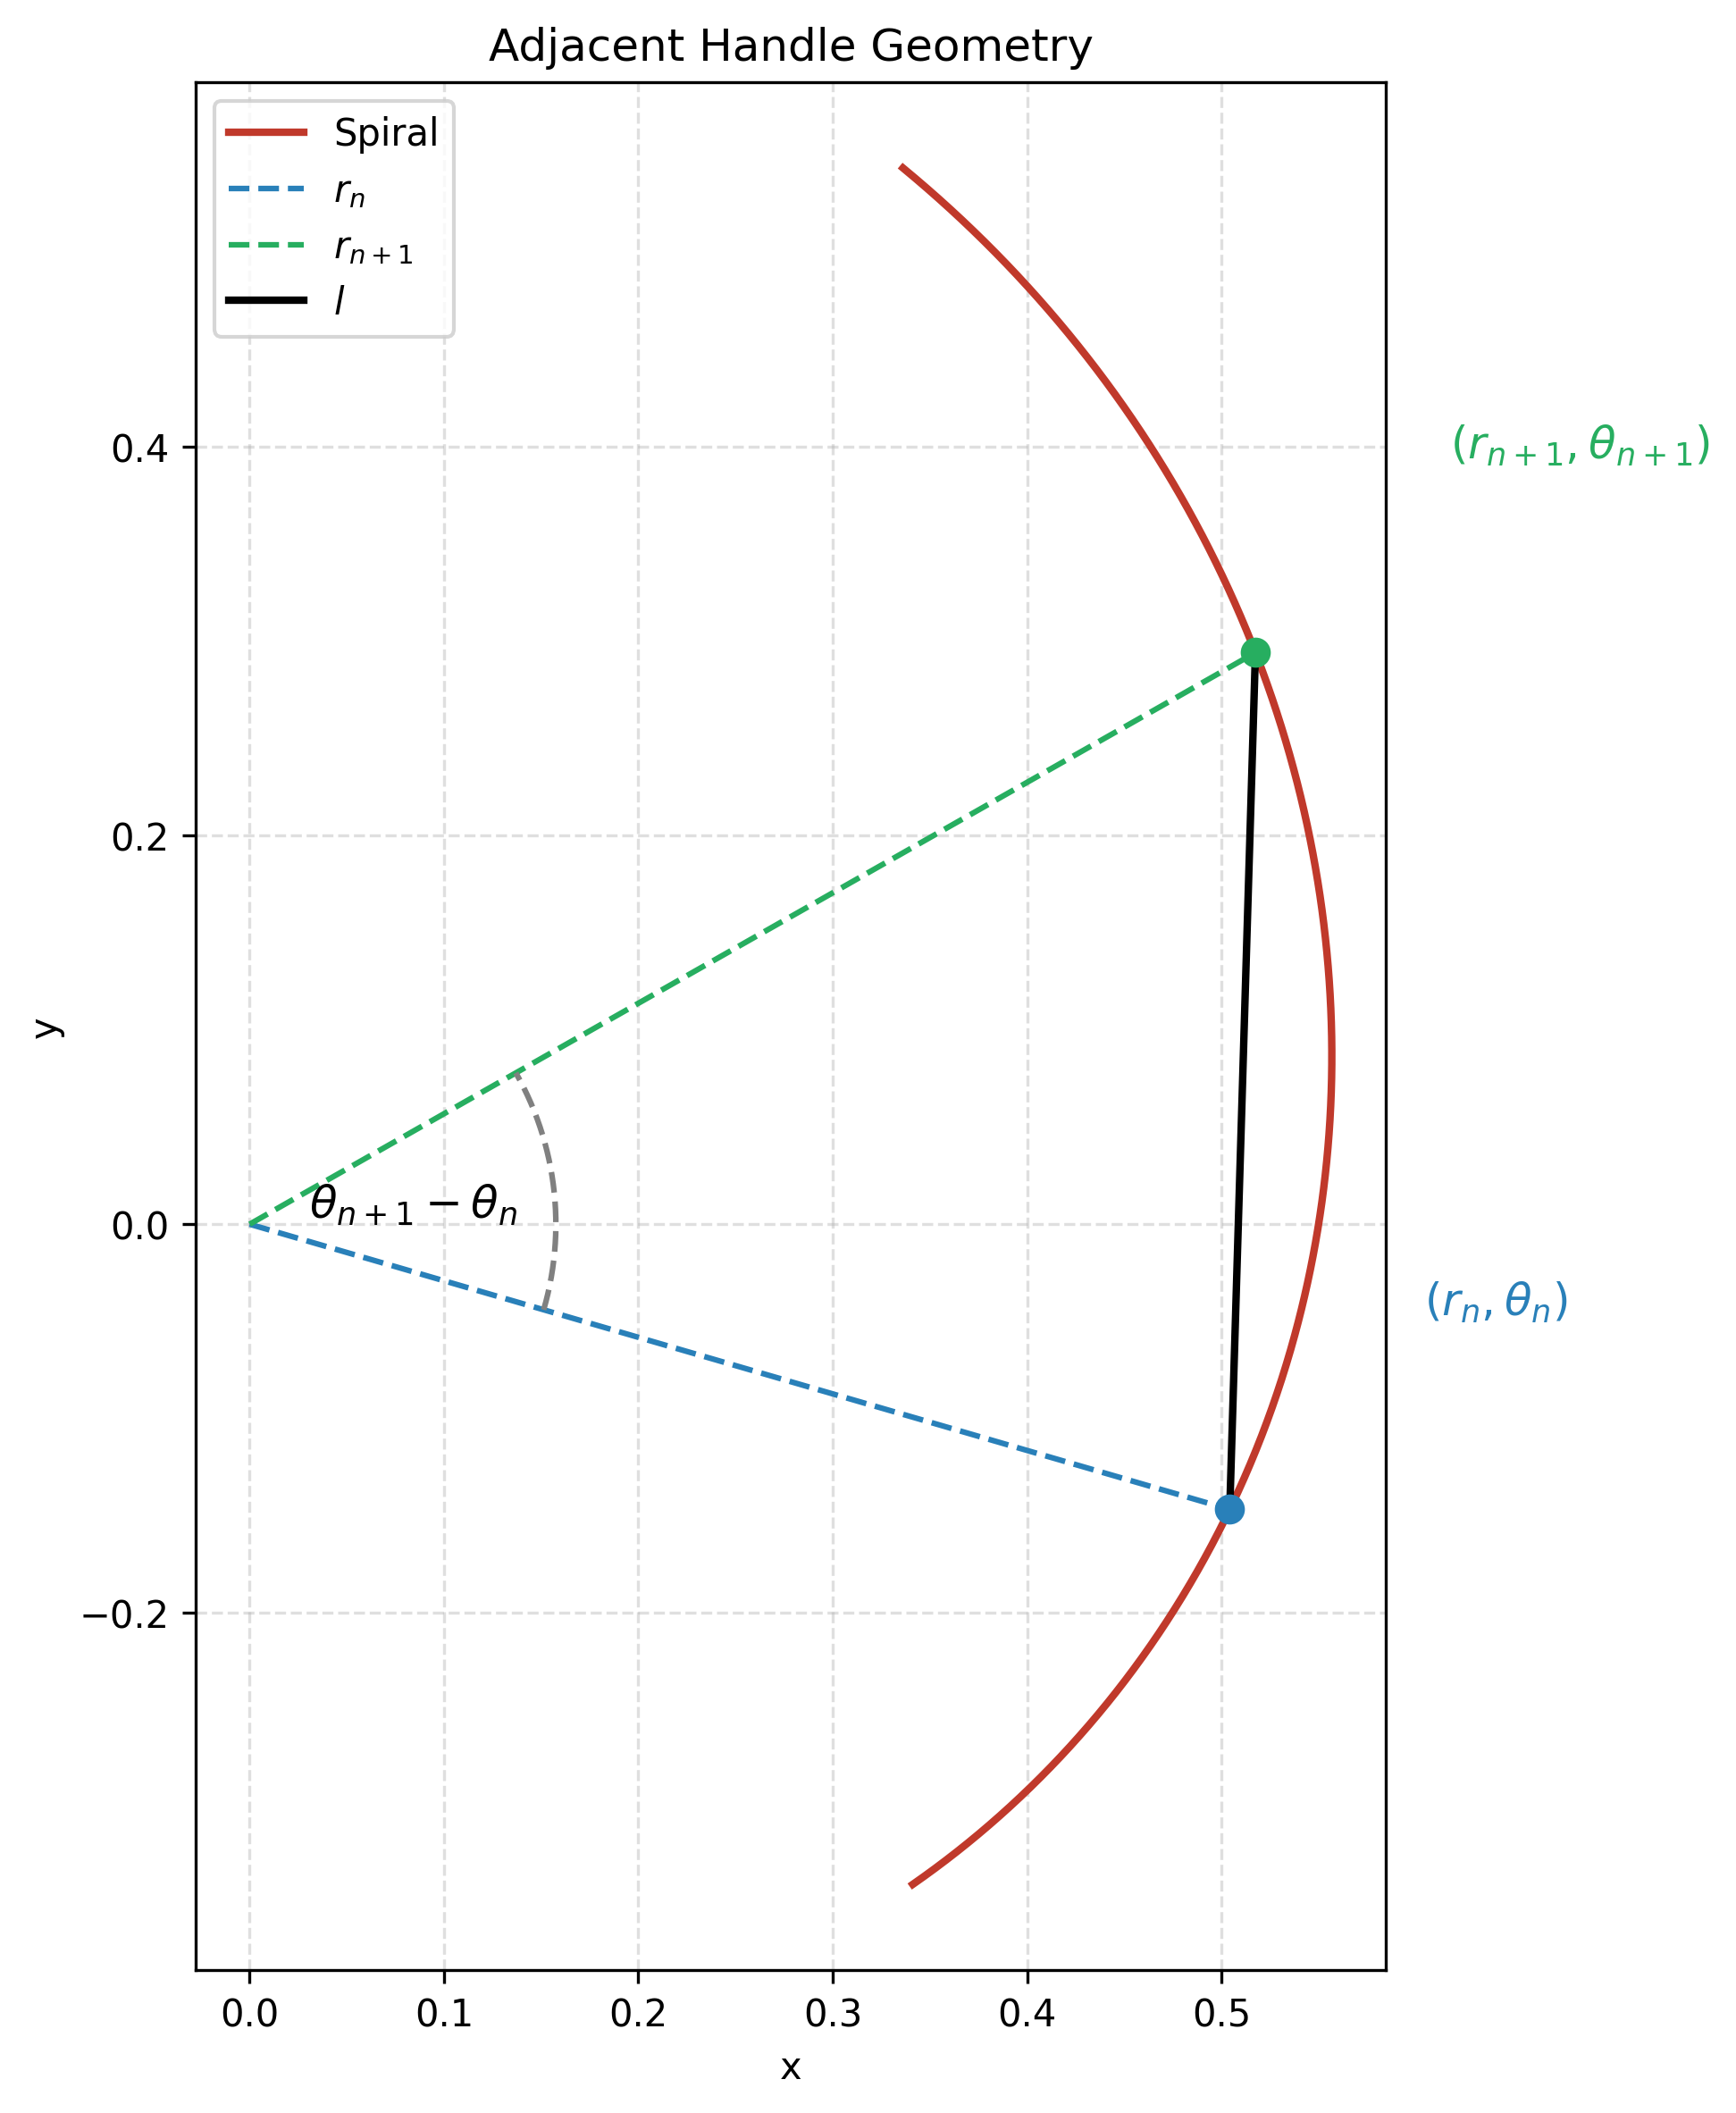
\includegraphics[width=0.62\textwidth]{图片和数据/plot2.png}
\caption{问题一相邻把手几何关系示意}
\label{fig:p1_adjacent_geom}
\end{figure}

\subsubsection{全体把手的直角坐标表示}
当各把手极角 $\theta_n(t)$ 求出后，即可得到对应极径
\begin{equation}
r_n(t)=a\theta_n(t),
\end{equation}
从而得到各把手的平面直角坐标
\begin{equation}
x_n(t)=a\theta_n(t)\cos\theta_n(t),
\end{equation}
\begin{equation}
y_n(t)=a\theta_n(t)\sin\theta_n(t).
\end{equation}

\paragraph{*Python任务3：}
将所有把手的极角结果批量转换为直角坐标，输出题目要求的关键位置，包括龙头前把手、龙尾前后把手及各节龙身前把手在 $0$--$300\,\mathrm{s}$ 每秒时刻的坐标。

\subsubsection{各把手速度模型}
由于各把手位置已表示为时间的函数，因此可进一步求解其瞬时速度。本文采用离散差分法近似计算：
\begin{equation}
v_n(t)\approx
\frac{\sqrt{\left[x_n(t+\Delta t)-x_n(t)\right]^2+\left[y_n(t+\Delta t)-y_n(t)\right]^2}}{\Delta t}.
\end{equation}

当时间步长 $\Delta t$ 取得足够小时，上式可较好逼近把手的瞬时速度。

若仅需输出整数秒时刻的速度，则可先在更小步长下进行数值模拟，再提取整数秒对应结果，以提高计算精度。

\paragraph{*Python任务4：}
采用较小时间步长（如 $\Delta t=0.01\,\mathrm{s}$ 或更小）进行数值计算，再提取整数秒结果，得到各把手在 $t=0,1,2,\dots,300$ 时刻的速度值，并整理成结果表格。

\subsubsection{问题一的求解流程}
综上，问题一的求解流程如下：

\begin{enumerate}
    \item 根据龙头前把手恒速盘入条件，求解其极角函数 $\theta_0(t)$；
    \item 根据龙头前把手的极角，求得龙头前把手位置；
    \item 利用相邻把手固定距离约束，逐节递推求出其余把手的极角；
    \item 将各把手极坐标转换为直角坐标；
    \item 通过差分法计算各把手速度；
    \item 输出题目要求的关键时刻与关键位置结果。
\end{enumerate}

\subsubsection{问题一模型的特点}
该模型以龙头轨迹为基础，通过刚体距离约束递推求出全队状态，结构清晰，便于程序实现。其优点在于：
\begin{itemize}
    \item 几何意义明确，便于解释板凳龙的盘入机制；
    \item 所有把手位置均由统一的递推关系得到，便于扩展；
    \item 可直接与后续碰撞检测、最小螺距求解及调头路径分析衔接。
\end{itemize}

但该模型也存在一定局限性：其一，假设板凳均为刚体，忽略连接处柔性形变；其二，速度采用离散差分近似，结果受时间步长影响。因此，在后续数值实验中需结合步长敏感性分析验证结果的稳定性。

\subsubsection{结果输出说明}
在完成上述计算后，应整理得到以下结果：
\begin{enumerate}
    \item 龙头前把手在 $0$--$300\,\mathrm{s}$ 内每秒的位置与速度；
    \item 各节龙身前把手在 $0$--$300\,\mathrm{s}$ 内每秒的位置与速度；
    \item 龙尾前把手、龙尾后把手在 $0$--$300\,\mathrm{s}$ 内每秒的位置与速度。
\end{enumerate}

\noindent 这些结果可进一步整理为表格，并绘制龙头轨迹图、若干时刻队形图以及速度变化图，为后续问题二的碰撞分析提供基础数据支持。

进一步地，可将题目要求的若干代表性把手在关键时刻的坐标整理成表，以便与图形结果交叉验证。表~\ref{tab:handle_positions} 汇总了龙头、若干代表性龙身以及龙尾前后把手在 $0,60,120,180,240,300\,\mathrm{s}$ 时刻的位置结果。

\begin{table}[H]
\centering
\caption{部分把手坐标随时间变化情况}
\label{tab:handle_positions}
\begin{tabular}{lrrrrrr}
\toprule
 & 0 s & 60 s & 120 s & 180 s & 240 s & 300 s \\
\midrule
龙头 $x$ (m) & 8.800000 & 5.799209 & -4.084887 & -2.963609 & 2.594494 & 4.420274 \\
龙头 $y$ (m) & -0.000000 & -5.771092 & -6.304479 & 6.094780 & -5.356743 & 2.320429 \\
第 1 节龙身 $x$ (m) & 8.363824 & 7.456758 & -1.445473 & -5.237118 & 4.821221 & 2.459489 \\
第 1 节龙身 $y$ (m) & 2.826544 & -3.440399 & -7.405883 & 4.359627 & -3.561949 & 4.402476 \\
第 51 节龙身 $x$ (m) & -9.518732 & -8.686317 & -5.543150 & 2.890455 & 5.980011 & -6.301346 \\
第 51 节龙身 $y$ (m) & 1.341137 & 2.540108 & 6.377946 & 7.249289 & -3.827758 & 0.465829 \\
第 101 节龙身 $x$ (m) & 2.913983 & 5.687116 & 5.361939 & 1.898794 & -4.917371 & -6.237722 \\
第 101 节龙身 $y$ (m) & -9.918311 & -8.001384 & -7.557638 & -8.471614 & -6.379874 & 3.936008 \\
第 151 节龙身 $x$ (m) & 10.861726 & 6.682311 & 2.388757 & 1.005154 & 2.965378 & 7.040740 \\
第 151 节龙身 $y$ (m) & 1.828753 & 8.134544 & 9.727411 & 9.424751 & 8.399721 & 4.393013 \\
第 201 节龙身 $x$ (m) & 4.555102 & -6.619664 & -10.627211 & -9.287720 & -7.457151 & -7.458662 \\
第 201 节龙身 $y$ (m) & 10.725118 & 9.025570 & 1.359847 & -4.246673 & -6.180726 & -5.263384 \\
龙尾（前） $x$ (m) & -6.722522 & 6.019090 & 10.963950 & 8.454187 & 4.746919 & 3.367953 \\
龙尾（前） $y$ (m) & -9.831368 & -9.753092 & -0.806494 & 6.236593 & 8.794903 & 8.835478 \\
龙尾（后） $x$ (m) & -5.305444 & 7.364557 & 10.974348 & 7.383896 & 3.241051 & 1.785033 \\
龙尾（后） $y$ (m) & -10.676584 & -8.797992 & 0.843473 & 7.492370 & 9.469336 & 9.301164 \\
\bottomrule
\end{tabular}
\end{table}


为便于直观展示，图~\ref{fig:p1_head_traj} 给出了龙头在全时域内的盘入轨迹；图~\ref{fig:p1_pos_compare} 对比了龙头与龙尾前把手在平面上的轨迹差异，体现了刚体链跟随造成的空间滞后特征。

\begin{figure}[H]
\centering
\begin{tikzpicture}
\begin{axis}[
    width=0.72\textwidth,
    height=0.48\textwidth,
    xlabel={$x$ / m}, ylabel={$y$ / m},
    title={问题一：龙头前把手盘入轨迹},
    grid=both, axis equal image
]
\addplot[
    blue,
    thick,
    no marks,
    mark repeat=100000
]
table[
    col sep=comma,
    x=x_0,
    y=y_0,
    each nth point={100}
] {图片和数据/task1_head_trajectory_full.csv};
\end{axis}
\end{tikzpicture}
\caption{问题一龙头前把手完整轨迹}
\label{fig:p1_head_traj}
\end{figure}

\begin{figure}[H]
\centering
\begin{tikzpicture}
\begin{axis}[
    width=0.72\textwidth,
    height=0.48\textwidth,
    xlabel={$x$ / m}, ylabel={$y$ / m},
    title={问题一：龙头与龙尾前把手轨迹对比},
    grid=both, axis equal image,
    legend pos=south west
]
\addplot[red,thick,no marks] table[col sep=comma,x=head_front_x,y=head_front_y] {图片和数据/task3_positions_1s.csv};
\addplot[black,dashed,thick,no marks] table[col sep=comma,x=tail_front_x,y=tail_front_y] {图片和数据/task3_positions_1s.csv};
\legend{龙头前把手,龙尾前把手}
\end{axis}
\end{tikzpicture}
\caption{问题一关键把手轨迹对比}
\label{fig:p1_pos_compare}
\end{figure}

除平面轨迹外，还可以从参数演化和速度分布两个角度观察问题一结果。图~\ref{fig:p1_theta_time} 给出了若干代表性把手极角随时间的变化过程，反映出各把手在同一螺线上依次跟随、相位逐渐滞后的特征；图~\ref{fig:p1_speed_band} 给出了不同时间截面的把手速度分布，可用于观察速度沿队伍传播时的微小差异。

\begin{figure}[H]
\centering
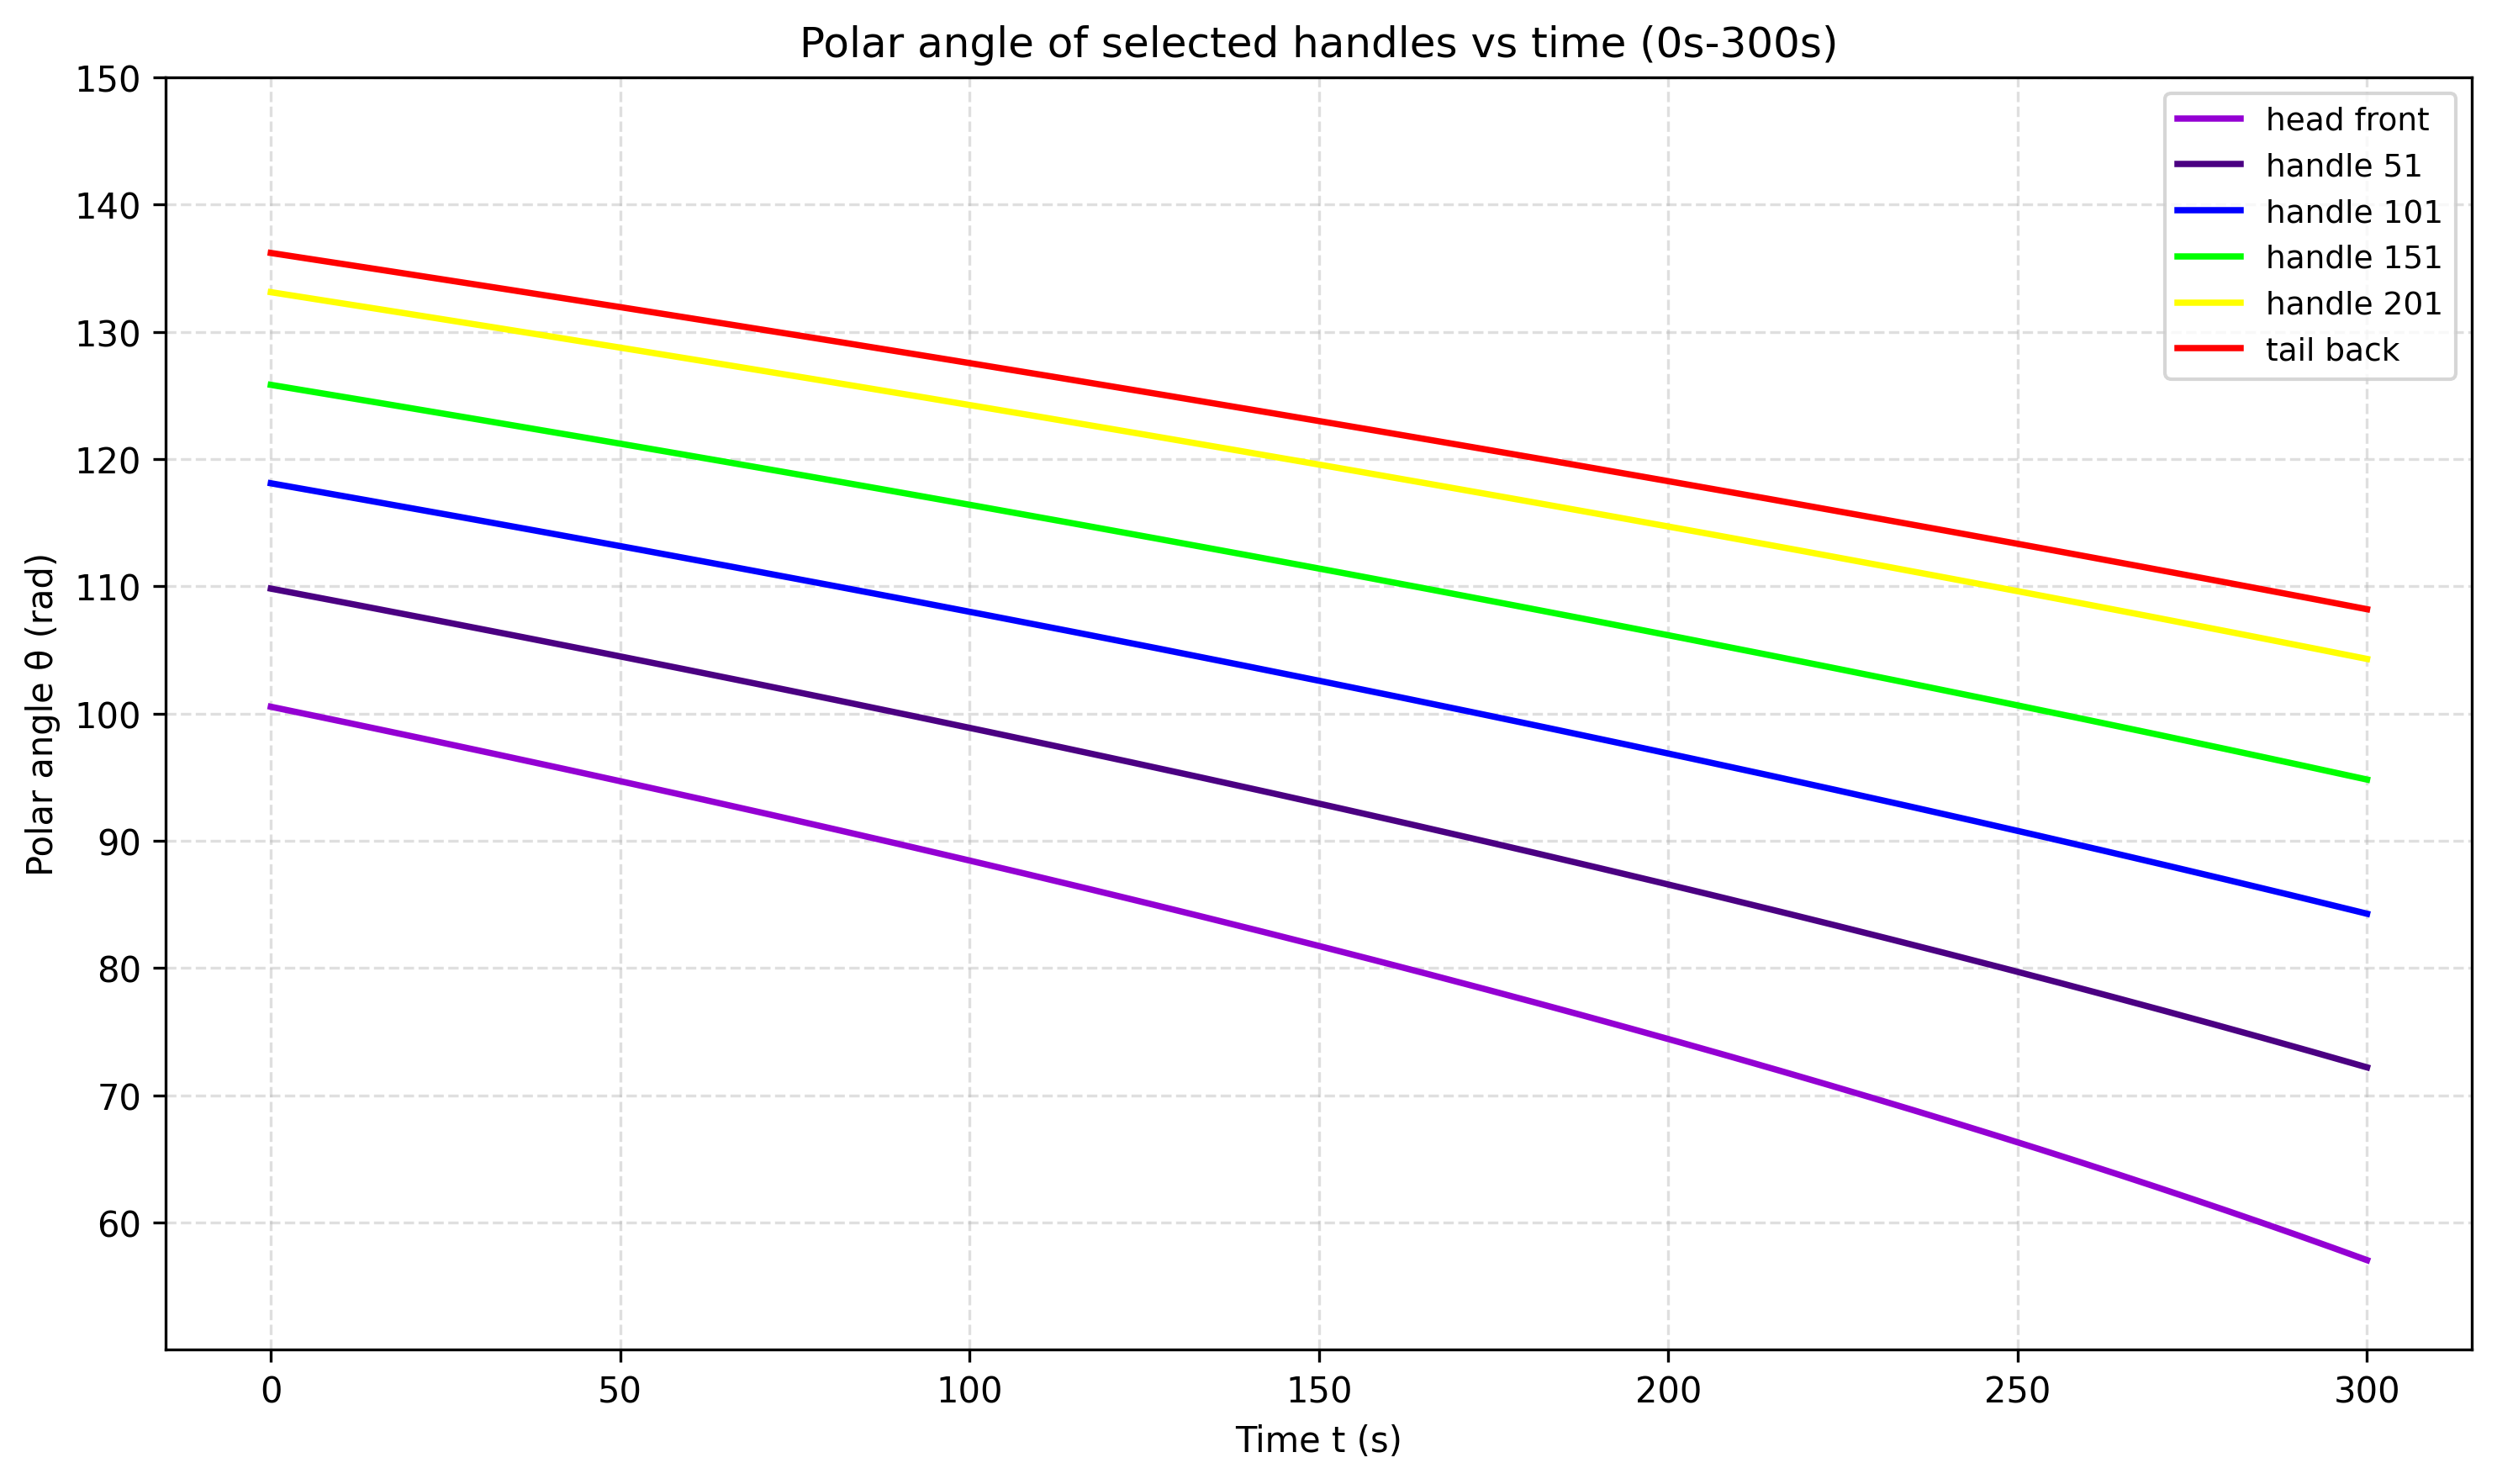
\includegraphics[width=0.78\textwidth]{图片和数据/plot5.png}
\caption{问题一代表性把手极角随时间变化}
\label{fig:p1_theta_time}
\end{figure}

\begin{figure}[H]
\centering
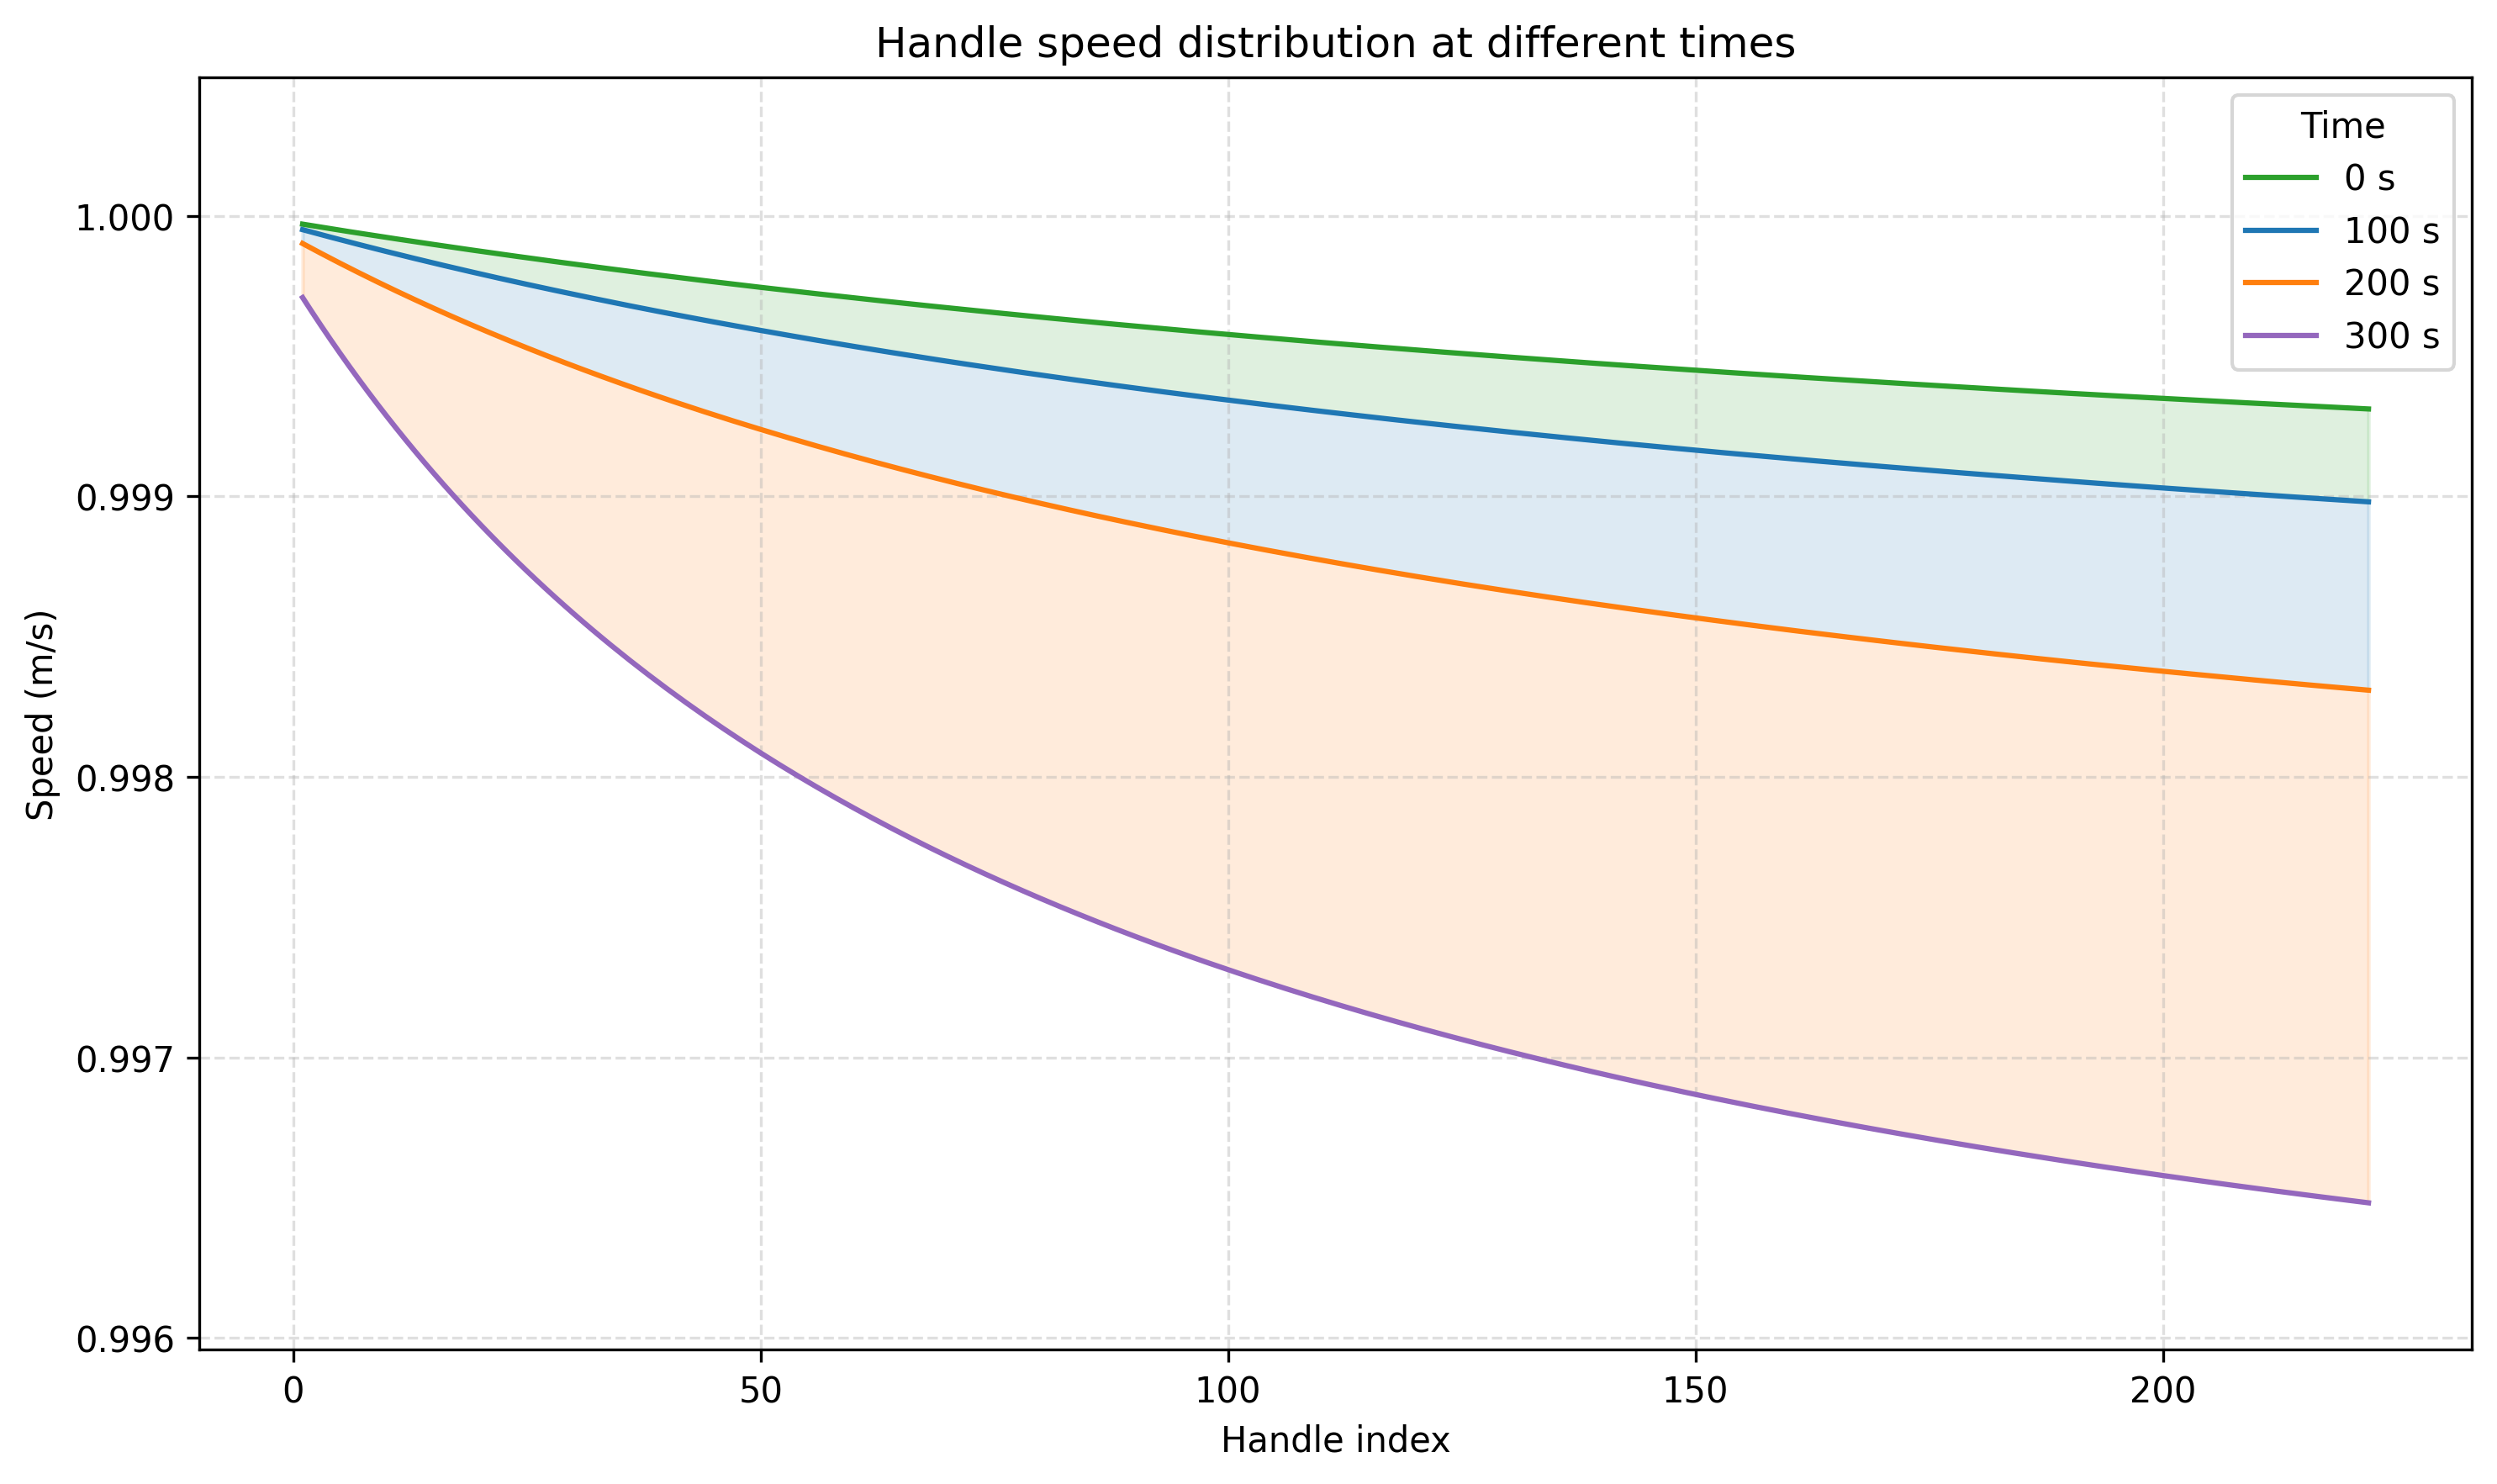
\includegraphics[width=0.82\textwidth]{图片和数据/plot4.png}
\caption{问题一不同时间下的把手速度分布}
\label{fig:p1_speed_band}
\end{figure}

\subsection{问题二：盘入过程中的碰撞判定}

\subsubsection{问题理解}
问题二要求在问题一已求得板凳龙各把手位置与速度的基础上，进一步判断板凳龙在持续盘入过程中是否会发生自碰撞，并给出首次碰撞时刻及相应位置特征。与问题一相比，问题二的关键变化在于：不仅要考虑把手这一系列离散点的位置，还必须考虑每节板凳本体具有有限长度和宽度，因此需要建立板凳实体的几何表示，并设计合理的碰撞判定准则。

从建模角度看，问题二的本质是一个\textbf{随时间变化的多刚体平面碰撞检测问题}。其核心步骤包括：
\begin{enumerate}
    \item 根据把手位置恢复每节板凳的几何区域；
    \item 对非相邻板凳进行空间相交或最小距离检测；
    \item 在时间轴上搜索首次碰撞发生的时刻。
\end{enumerate}

\subsubsection{模型建立思路}
问题二可分解为如下三个层次：

\begin{enumerate}
    \item \textbf{几何层：}将每节板凳由“前后把手”抽象为一个具有固定长度和宽度的矩形区域；
    \item \textbf{判定层：}给出任意两节板凳是否碰撞的数学准则；
    \item \textbf{搜索层：}沿时间轴逐步检测，确定首次碰撞时刻。
\end{enumerate}

因此，问题二的建模逻辑可概括为
\[
\text{把手位置} \longrightarrow \text{板凳矩形重建} \longrightarrow \text{两两碰撞检测} \longrightarrow \text{首次碰撞搜索}.
\]

\subsubsection{板凳的几何抽象}
设第 $n$ 节板凳对应的前后把手坐标分别为
\[
P_n^{(f)}=(x_n^{(f)},y_n^{(f)}), \qquad
P_n^{(b)}=(x_n^{(b)},y_n^{(b)}).
\]
则该节板凳的中心线方向向量可写为
\begin{equation}
\bm{u}_n=
\frac{1}{\sqrt{\left(x_n^{(b)}-x_n^{(f)}\right)^2+\left(y_n^{(b)}-y_n^{(f)}\right)^2}}
\begin{pmatrix}
x_n^{(b)}-x_n^{(f)}\\
y_n^{(b)}-y_n^{(f)}
\end{pmatrix}.
\end{equation}

对应的单位法向量记为
\begin{equation}
\bm{v}_n=
\begin{pmatrix}
-u_{n,2}\\
u_{n,1}
\end{pmatrix}.
\end{equation}

设板凳宽度为 $w$，则矩形四个顶点可表示为
\begin{equation}
A_n=P_n^{(f)}+\frac{w}{2}\bm{v}_n,
\qquad
B_n=P_n^{(f)}-\frac{w}{2}\bm{v}_n,
\end{equation}
\begin{equation}
C_n=P_n^{(b)}-\frac{w}{2}\bm{v}_n,
\qquad
D_n=P_n^{(b)}+\frac{w}{2}\bm{v}_n.
\end{equation}

于是，第 $n$ 节板凳可抽象为平面矩形区域
\begin{equation}
\Omega_n=\text{Rect}(A_n,B_n,C_n,D_n).
\end{equation}

这一表示方式保留了板凳长度、朝向与宽度信息，可用于后续碰撞检测。

\paragraph{*Python任务1：}
基于问题一中已求得的各把手坐标，编写程序在每个时刻重建所有板凳的矩形区域 $\Omega_n$，输出每节板凳四个顶点坐标，作为碰撞检测的几何输入。


为了更直观地说明板凳实体化后的几何含义，图~\ref{fig:p2_board_geom} 给出了单节板凳在某一时刻的局部示意：由前后把手确定中心线方向，再沿法向扩展得到板凳宽度，并进一步标出碰撞检测中使用的辅助点。该图与上文矩形区域 $\Omega_n$ 的定义是一一对应的。

\begin{figure}[H]
\centering
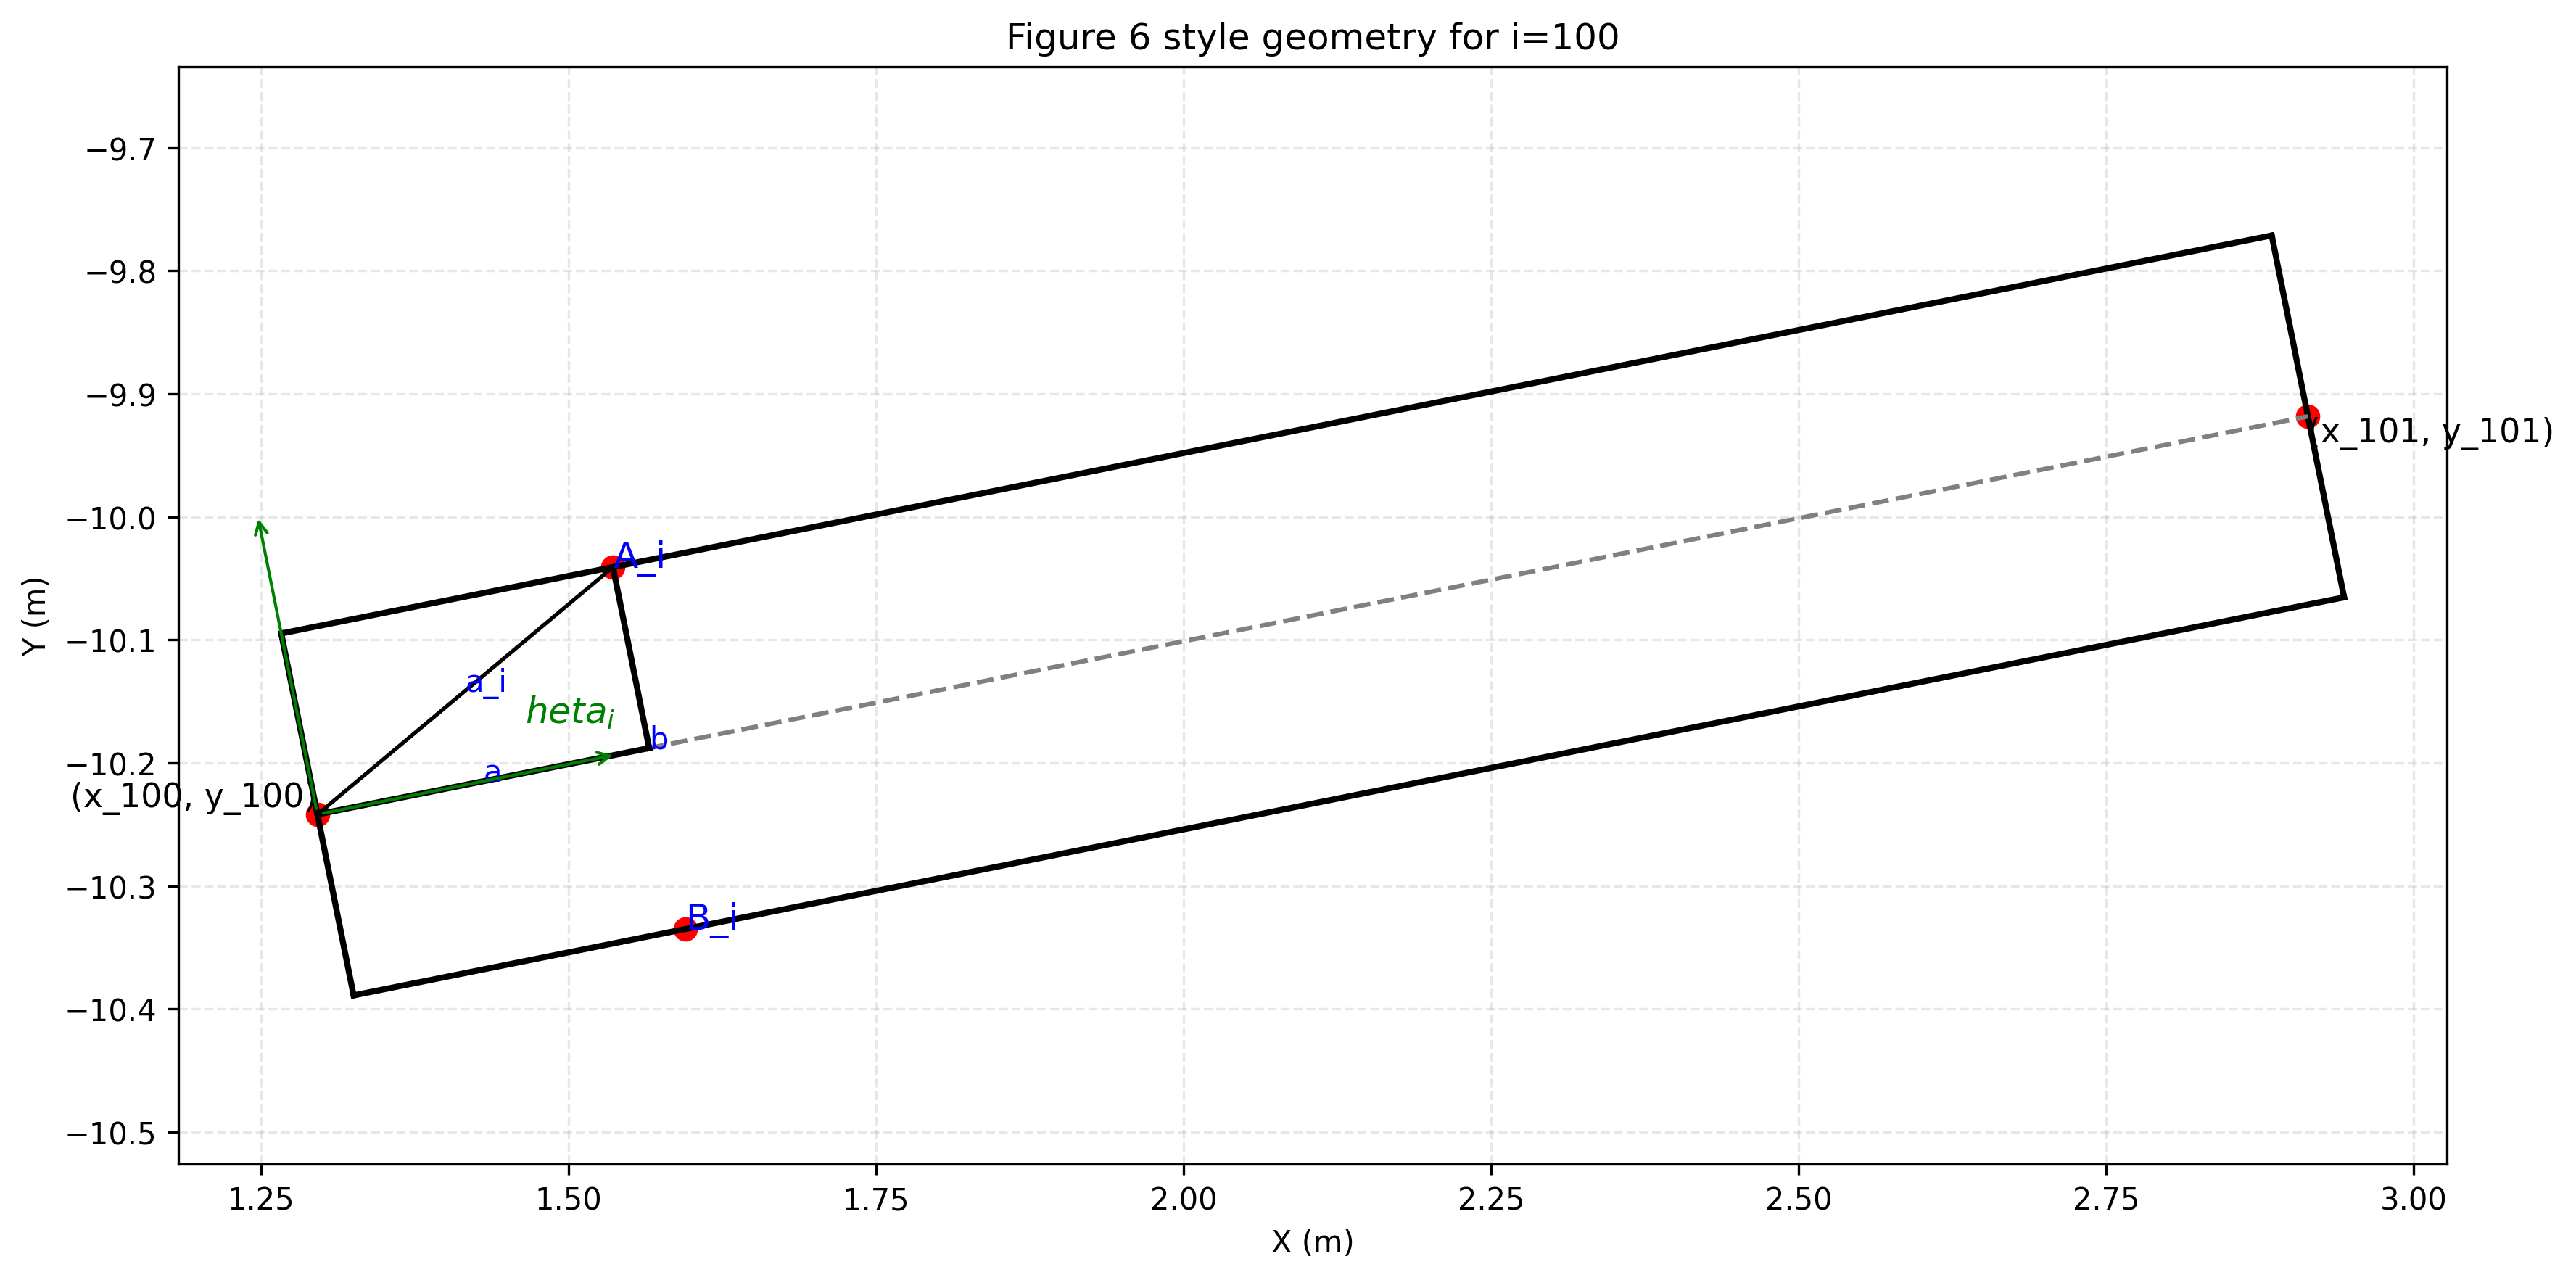
\includegraphics[width=0.82\textwidth]{图片和数据/plot6.png}
\caption{问题二单节板凳几何抽象示意}
\label{fig:p2_board_geom}
\end{figure}

\subsubsection{候选碰撞对象的筛选}
由于相邻板凳之间通过结构连接，本身存在端点接触，因此碰撞检测时通常无需判断相邻两节板凳是否“碰撞”。为避免无效计算，仅考虑满足
\begin{equation}
|i-j|>1
\end{equation}
的非相邻板凳对 $(\Omega_i,\Omega_j)$。

进一步地，由于板凳龙沿螺线盘入，最有可能发生碰撞的是\textbf{空间上相近但编号相隔较远}的板凳，因此可引入预筛选机制：若两节板凳中心点距离大于某一阈值，则直接判定其不可能碰撞，从而降低计算复杂度。

设第 $n$ 节板凳的中心点为
\begin{equation}
M_n=\frac{P_n^{(f)}+P_n^{(b)}}{2}.
\end{equation}
若存在阈值 $R_0$，使得
\begin{equation}
\|M_i-M_j\|>R_0,
\end{equation}
则可认为 $\Omega_i$ 与 $\Omega_j$ 在当前时刻不发生碰撞。

\paragraph{*Python任务2：}
对每个时刻的所有板凳对先进行候选筛选，仅保留满足 $|i-j|>1$ 且中心点距离较近的候选板凳对，减少后续精确碰撞检测的计算量。

\subsubsection{碰撞判定准则}
对于任意两节候选板凳 $\Omega_i$ 与 $\Omega_j$，若其区域存在交集，则认为在该时刻发生碰撞，即
\begin{equation}
\Omega_i \cap \Omega_j \neq \varnothing.
\end{equation}

在数值实现中，可采用如下两类判定方法。

\paragraph{方法一：矩形相交判定}
将每节板凳视为凸四边形，对任意两板凳采用分离轴定理（Separating Axis Theorem, SAT）进行判定。若不存在可将两矩形完全分开的投影轴，则认为两矩形相交，即发生碰撞。

设投影轴为单位向量 $\bm{e}$，矩形 $\Omega_n$ 的四个顶点在该方向上的投影区间记为
\begin{equation}
I_n(\bm{e})=
\left[
\min_{Q\in\{A_n,B_n,C_n,D_n\}}\langle Q,\bm{e}\rangle,\,
\max_{Q\in\{A_n,B_n,C_n,D_n\}}\langle Q,\bm{e}\rangle
\right].
\end{equation}
若对所有候选轴 $\bm{e}$ 都有
\begin{equation}
I_i(\bm{e})\cap I_j(\bm{e})\neq \varnothing,
\end{equation}
则两矩形相交。

\paragraph{方法二：最小距离阈值判定}
也可计算两矩形边界间的最小距离，记为
\begin{equation}
d_{ij}(t)=\operatorname{dist}(\Omega_i,\Omega_j).
\end{equation}
当
\begin{equation}
d_{ij}(t)\le 0
\end{equation}
时，表示两矩形相交；若考虑数值误差，也可设定小阈值 $\varepsilon>0$，当
\begin{equation}
d_{ij}(t)<\varepsilon
\end{equation}
时判定为发生碰撞。

在本文中，为保证判定的几何准确性，优先采用\textbf{矩形相交判定}作为主方法，并可用最小距离作为辅助验证。

\paragraph{*Python任务3：}
实现两节板凳矩形的精确碰撞检测函数。推荐优先实现基于 SAT 的矩形相交判定，并额外输出候选板凳对的最小距离，用于校验结果与分析碰撞发生前的接近过程。

\subsubsection{首次碰撞时刻的搜索}
在给定总模拟时间区间 $[0,T]$ 内，设碰撞指示函数为
\begin{equation}
C(t)=
\begin{cases}
1, & \text{若在时刻 } t \text{ 存在某对板凳发生碰撞},\\
0, & \text{否则}.
\end{cases}
\end{equation}
则首次碰撞时刻可定义为
\begin{equation}
t_c=\inf\{t\in[0,T]\mid C(t)=1\}.
\end{equation}

在数值计算中，可先采用较小时间步长 $\Delta t$ 对时间区间离散化，逐时刻检测是否发生碰撞。当首次检测到 $C(t_k)=1$ 时，即得到一个碰撞时刻近似值。为进一步提高精度，可在区间 $[t_{k-1},t_k]$ 内继续缩小步长，进行局部二分搜索或细网格搜索，以确定更准确的首次碰撞时刻。

\paragraph{*Python任务4：}
沿时间轴逐步检测碰撞状态，找到首次满足 $C(t)=1$ 的时间点，并在首次碰撞前后时间区间内进行局部加密搜索，输出更精确的首次碰撞时刻 $t_c$。

\subsubsection{首次碰撞位置的确定}
在首次碰撞时刻 $t_c$ 求出后，可进一步记录发生碰撞的板凳编号对 $(i,j)$，并提取其对应矩形顶点坐标、中心点坐标及局部最小距离等信息。若采用 SAT 或最小距离方法，也可进一步计算相交边或最接近点，从而描述碰撞发生的位置特征。

设首次碰撞对应板凳为 $\Omega_i$ 与 $\Omega_j$，则可输出如下几类信息：
\begin{enumerate}
    \item 首次碰撞时刻 $t_c$；
    \item 首次碰撞板凳编号 $(i,j)$；
    \item 碰撞时两板凳中心点坐标 $M_i(t_c),M_j(t_c)$；
    \item 碰撞时两板凳最小距离 $d_{ij}(t_c)$；
    \item 碰撞时整条板凳龙的空间形态图。
\end{enumerate}

\paragraph{*Python任务5：}
在首次碰撞时刻记录碰撞板凳编号、矩形顶点、中心点、最小距离等信息，并绘制首次碰撞时整条板凳龙的平面位置图，为后续结果展示提供图表支持。

\subsubsection{问题二的求解流程}
综上，问题二的求解流程如下：

\begin{enumerate}
    \item 利用问题一的结果，获得各时刻全部把手的平面坐标；
    \item 对每节板凳重建矩形区域，得到其几何表示；
    \item 筛选可能发生碰撞的非相邻板凳对；
    \item 对候选板凳对进行精确矩形相交检测；
    \item 沿时间轴搜索首次碰撞时刻；
    \item 输出首次碰撞时刻、碰撞板凳编号及碰撞位置特征。
\end{enumerate}

\subsubsection{问题二模型的特点}
该模型是在问题一运动学结果基础上的进一步扩展，其优势在于：
\begin{itemize}
    \item 将板凳抽象为矩形后，能够较真实地反映板凳实体宽度带来的碰撞风险；
    \item 将碰撞检测分为“候选筛选 + 精确判定”两个阶段，有利于提高程序运行效率；
    \item 首次碰撞时刻的搜索结果可直接为问题三中的最小螺距分析提供依据。
\end{itemize}

但模型也存在一定局限性：
\begin{itemize}
    \item 板凳被简化为理想矩形，未考虑端部圆角、连接件等结构细节；
    \item 碰撞判定依赖离散时间步长，若步长过大可能漏检瞬时碰撞；
    \item 首次碰撞时刻的精度依赖局部加密搜索策略。
\end{itemize}

因此，在数值实现中需要结合步长控制与结果复核来保证碰撞判定的可靠性。

\subsubsection{结果输出说明}
完成上述建模与计算后，应给出以下结果：
\begin{enumerate}
    \item 在给定盘入过程中是否发生碰撞；
    \item 首次碰撞时刻 $t_c$；
    \item 首次碰撞对应的板凳编号；
    \item 首次碰撞时整条板凳龙的平面形态图；
    \item 若需要，可给出首次碰撞前若干时刻的最小距离变化曲线。
\end{enumerate}

\noindent 这些结果不仅可以验证盘入路径的可行性，也为后续最小螺距优化与调头路径设计提供了关键依据。


从结果展示角度看，问题二至少应配合一幅局部构型图来解释“何谓碰撞”以及“碰撞是如何被检测出来的”。若后续补充了首次碰撞时刻的整队构型截图，则建议将其与图~\ref{fig:p2_board_geom} 配套放置：前者用于展示全局空间位置，后者用于说明局部判定依据。

结合数值仿真结果，可进一步从“首次碰撞构型”和“碰撞前最小距离演化”两个角度展示问题二的输出。图~\ref{fig:p2_collision_snapshot} 给出了首次碰撞附近的整队平面构型，其中橙色高亮部分对应发生危险接近的板凳对；图~\ref{fig:p2_min_clearance_curve} 则给出了碰撞前后最小距离随时间的变化过程，可用于读取首次越过安全阈值的关键时刻。

\begin{figure}[H]
\centering
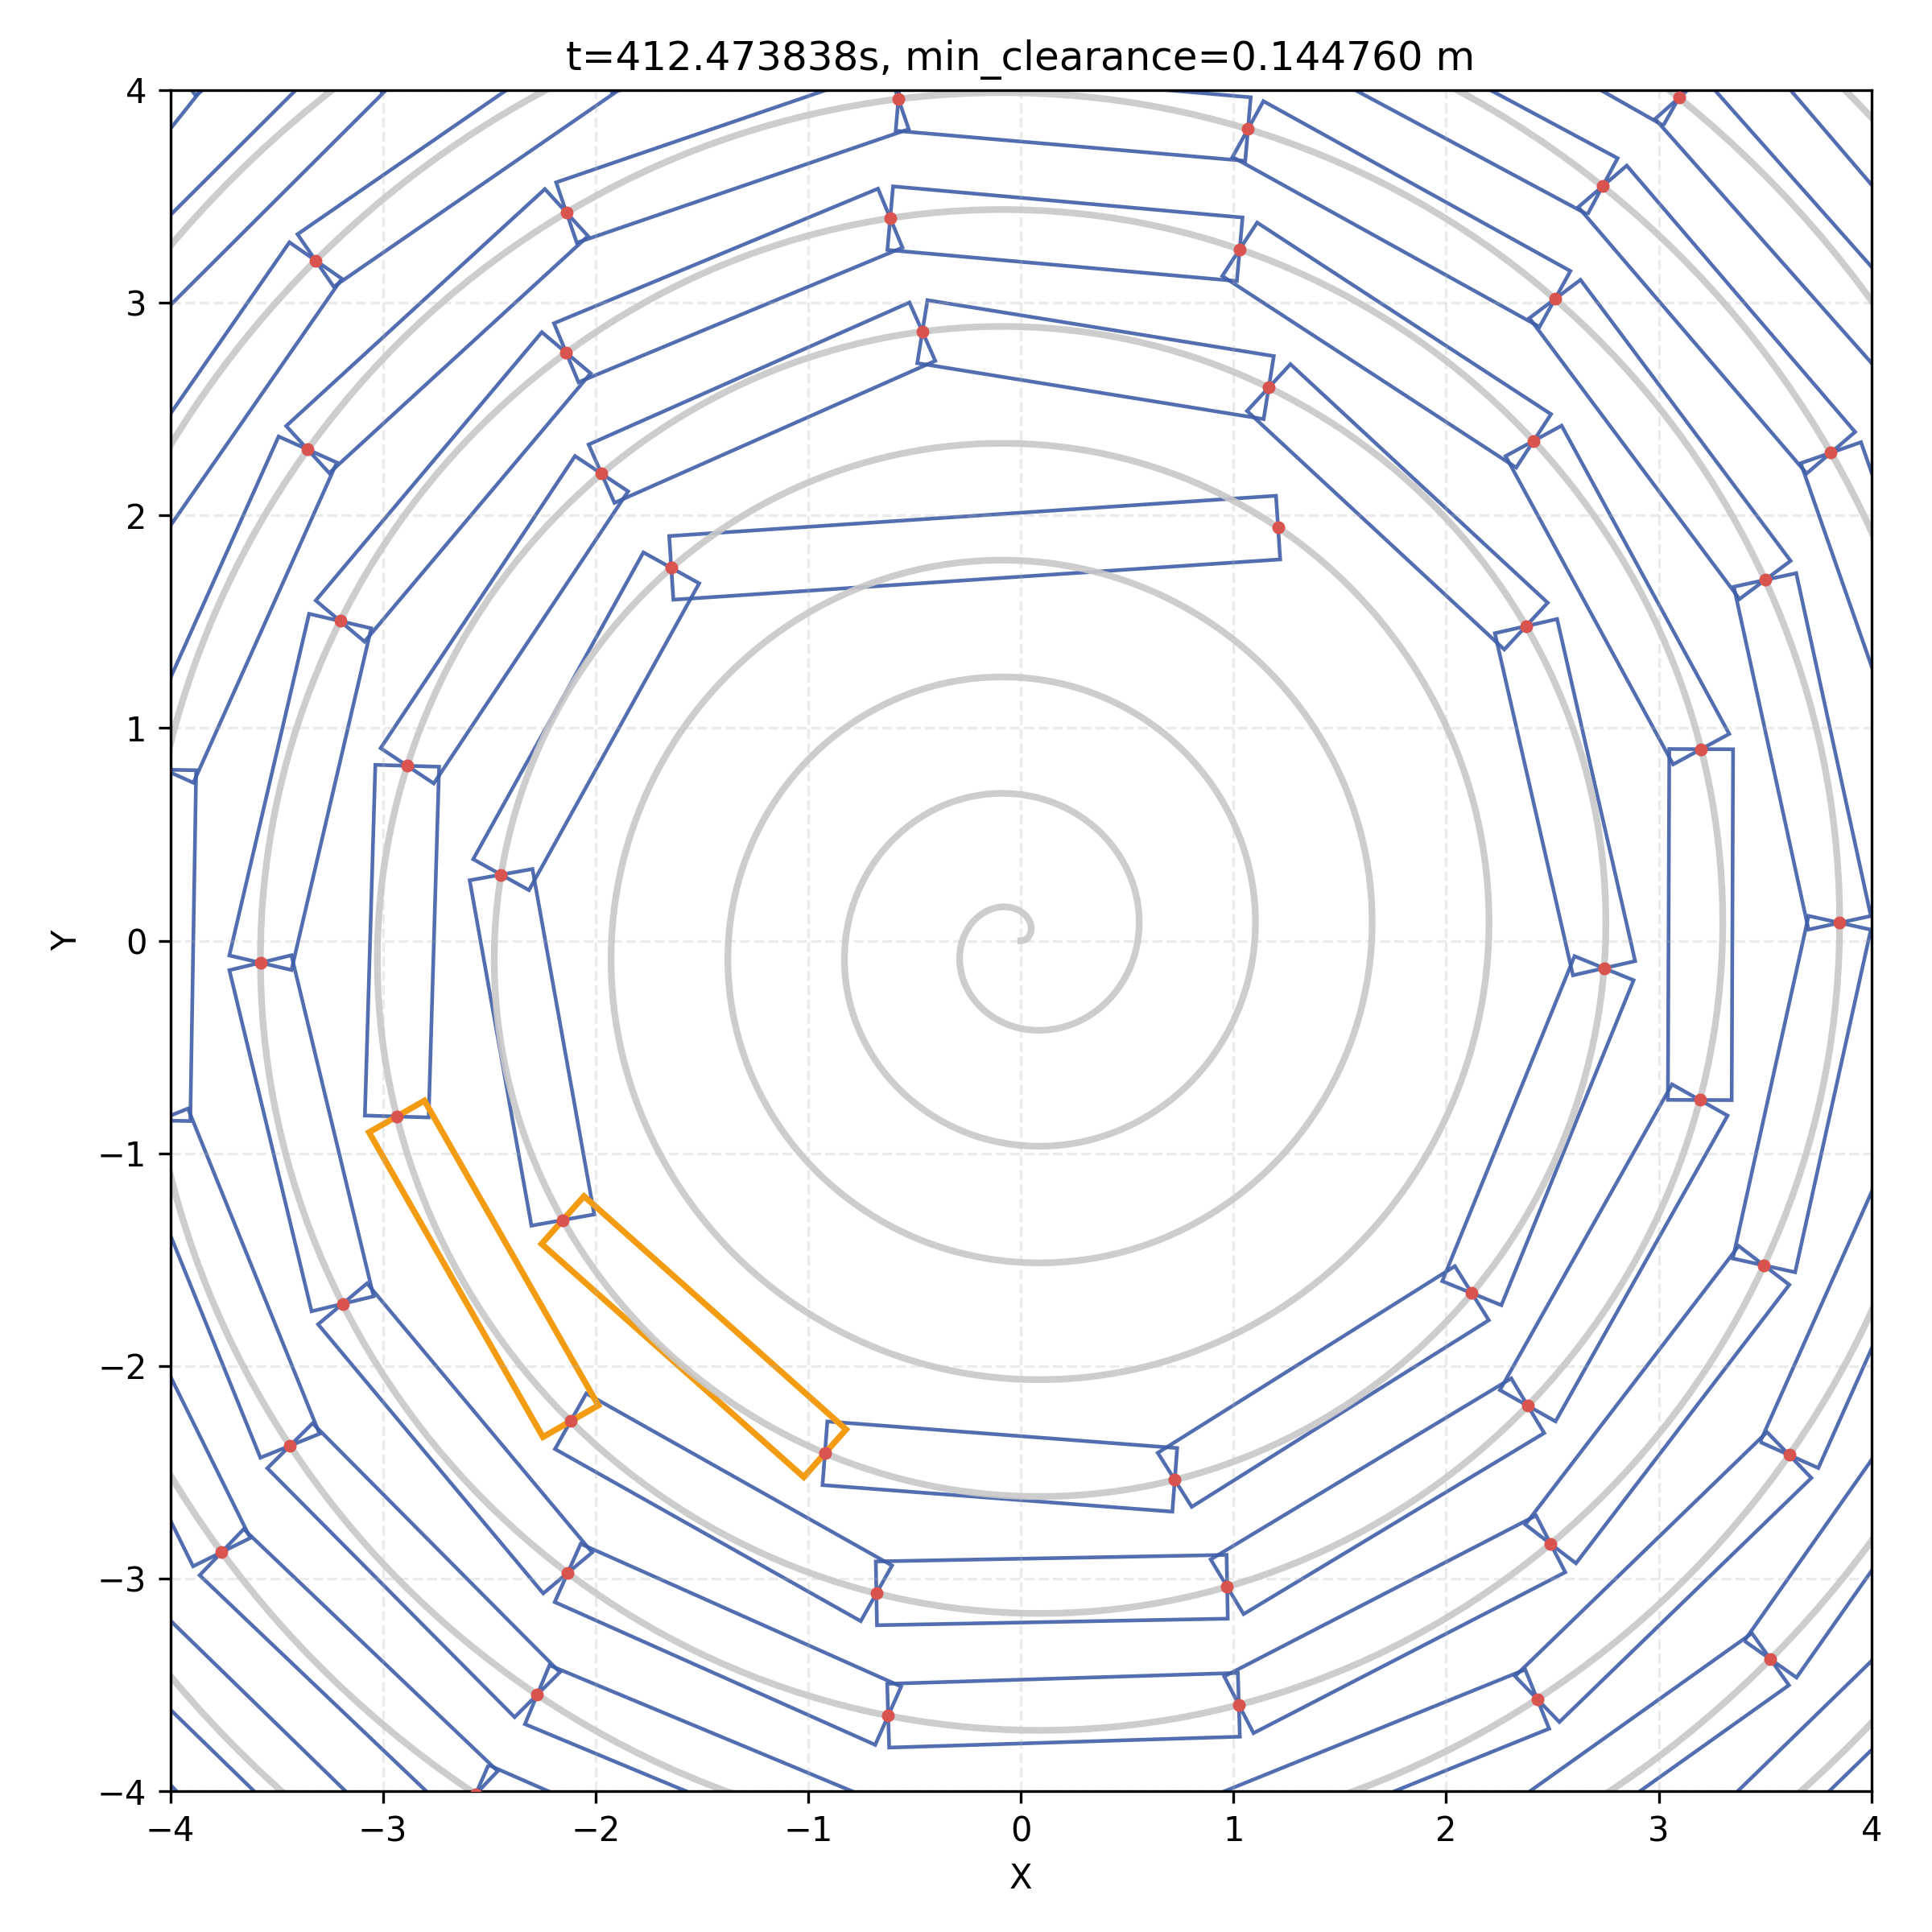
\includegraphics[width=0.82\textwidth]{plot8.png}
\caption{问题二首次碰撞附近的整队构型}
\label{fig:p2_collision_snapshot}
\end{figure}

\begin{figure}[H]
\centering
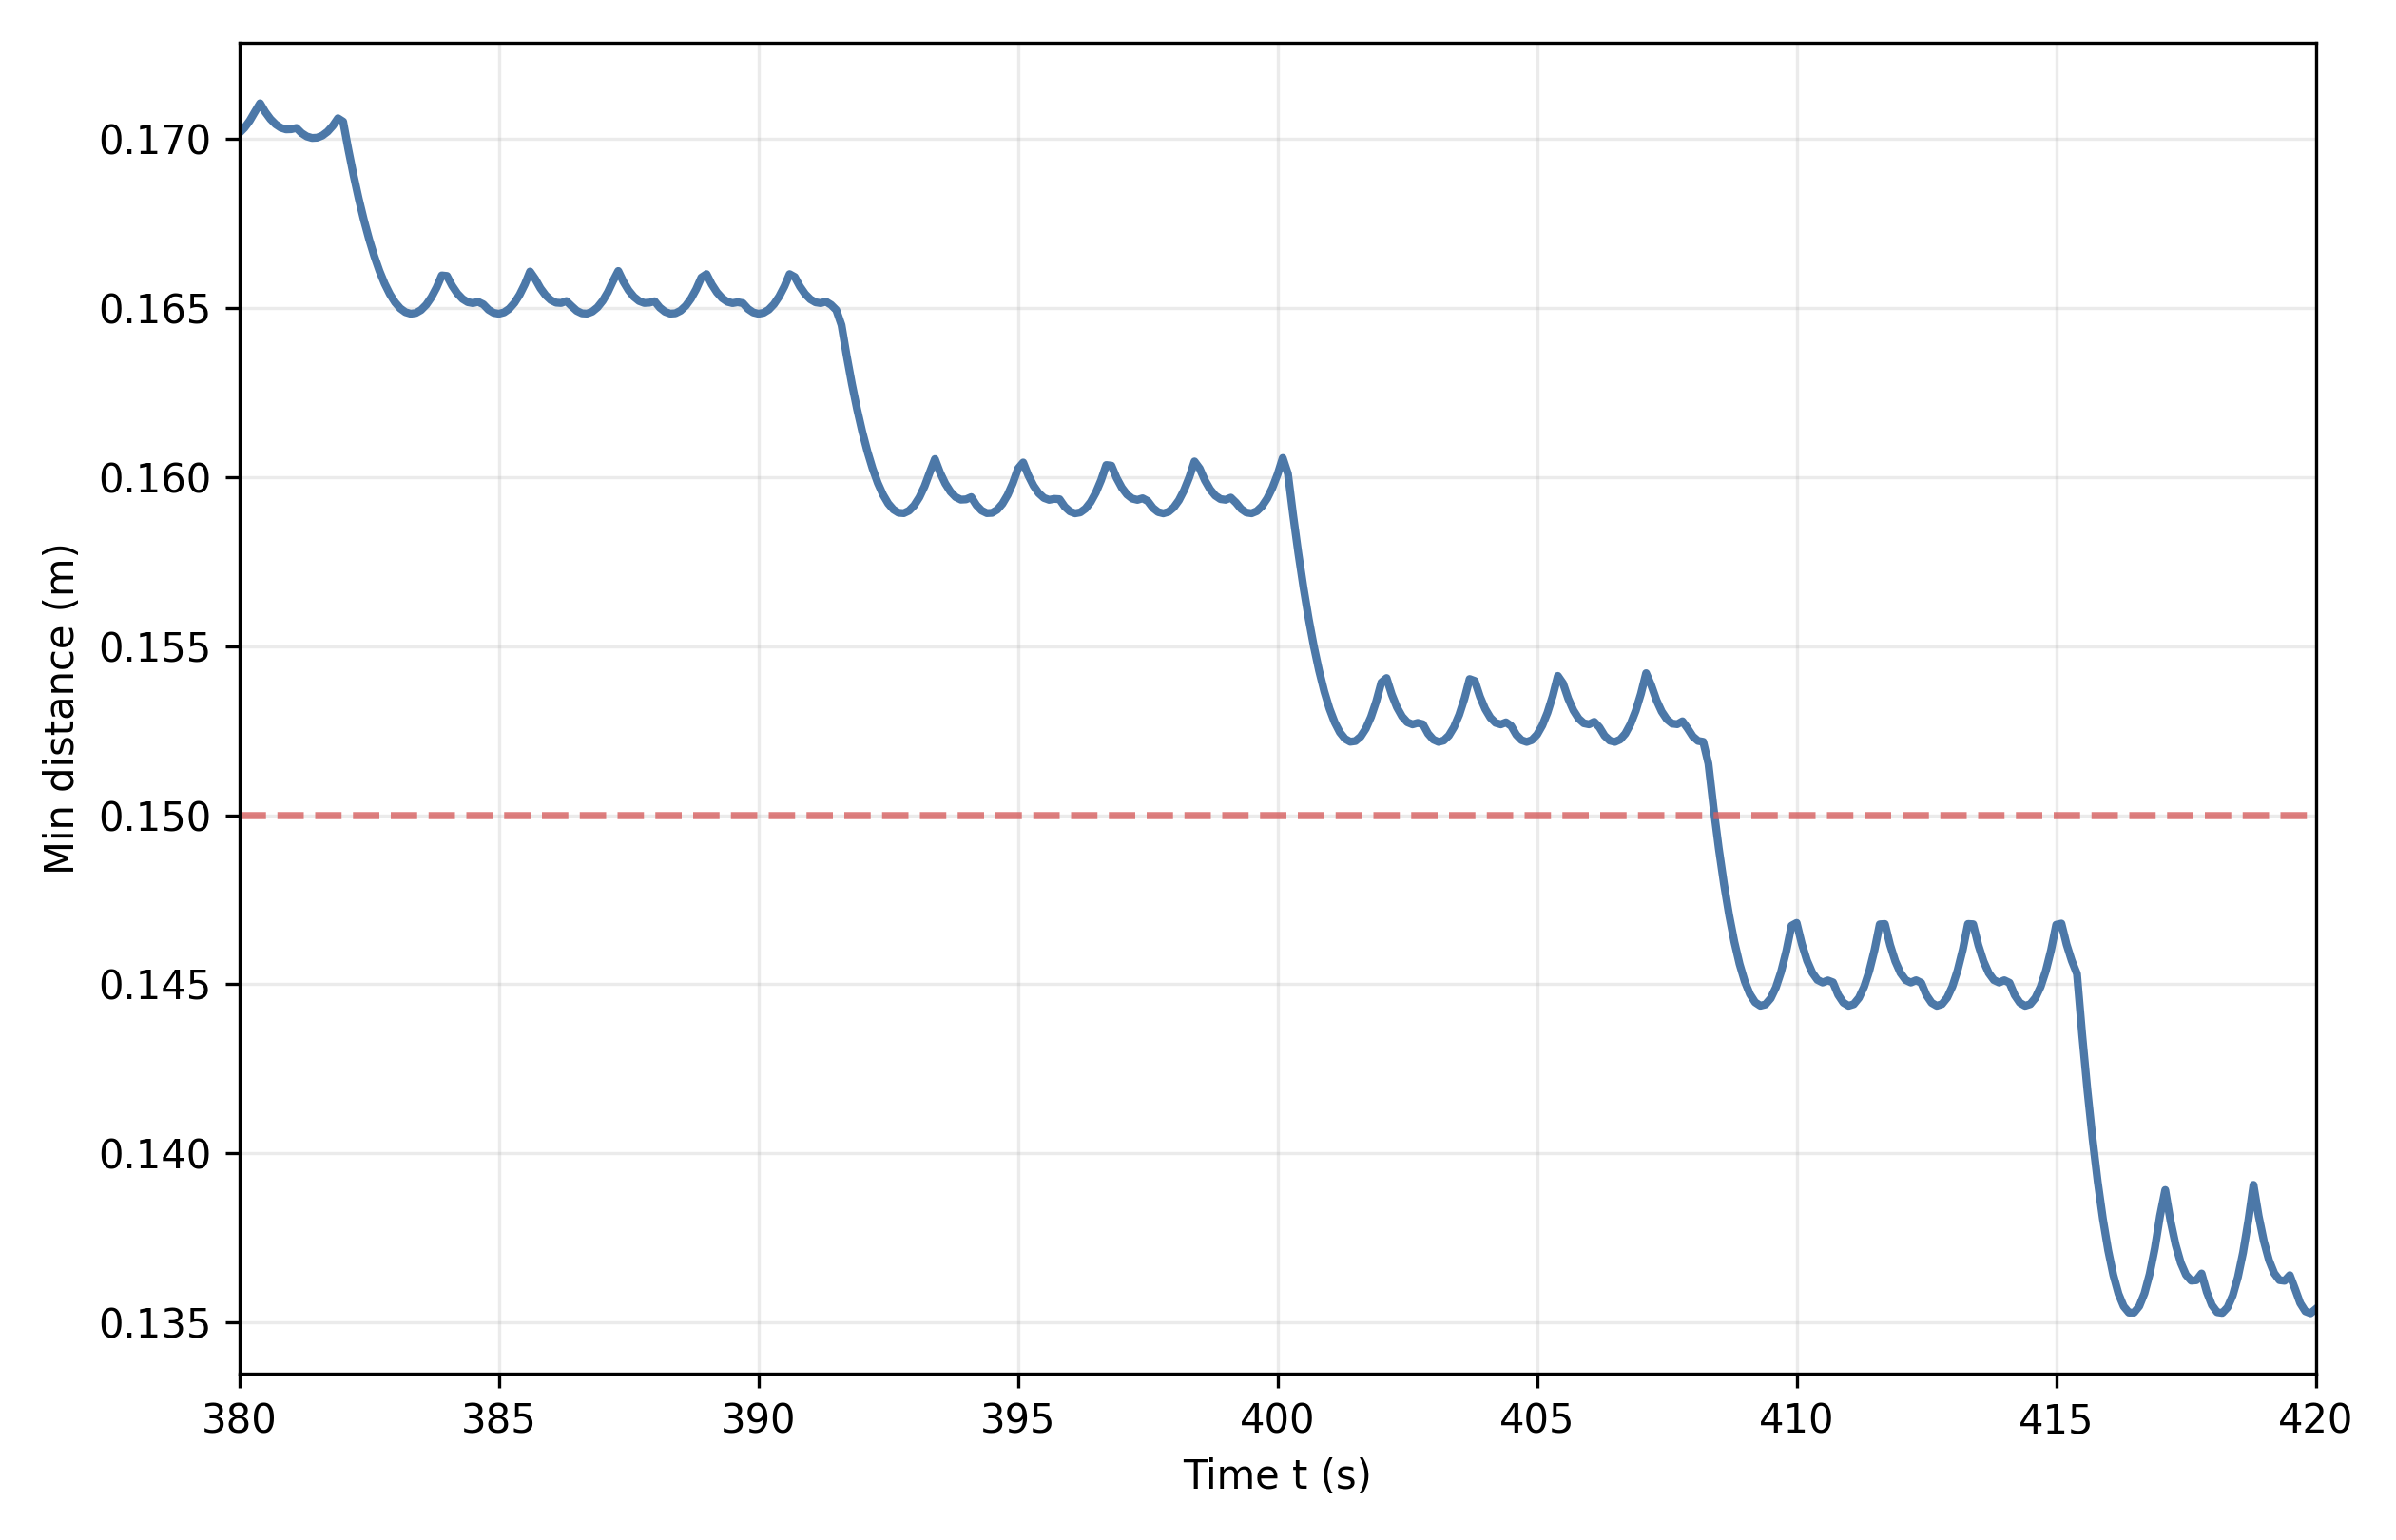
\includegraphics[width=0.88\textwidth]{plot9.png}
\caption{问题二最小距离随时间变化曲线}
\label{fig:p2_min_clearance_curve}
\end{figure}

\subsection{问题三：最小螺距求解}

\subsubsection{问题理解}
问题三要求在给定调头空间约束下，确定板凳龙在盘入过程中既能够进入指定区域、又不会发生自碰撞时所允许的最小螺距。与问题一、问题二相比，本问的核心不再是单次轨迹仿真，而是将螺距视为待优化参数，在可行性约束下寻找其下界。

从建模角度看，问题三本质上是一个\textbf{带几何可行性约束的参数优化问题}。其关键在于：螺距过大时，路径较松散，不利于缩小占地空间；螺距过小时，板凳龙相邻圈层之间距离变小，更容易在盘入过程中发生碰撞。因此，需要在“尽可能紧凑”和“避免碰撞”之间寻找平衡点。

\subsubsection{模型建立思路}
问题三可以分解为以下三个层次：

\begin{enumerate}
    \item \textbf{参数层：}将螺距 $d$ 视为决策变量；
    \item \textbf{可行性层：}对给定螺距，判断板凳龙是否能在盘入过程中安全进入调头空间；
    \item \textbf{优化层：}在所有可行螺距中寻找最小值。
\end{enumerate}

因此，问题三的建模逻辑可概括为
\[
\text{给定螺距 } d \longrightarrow \text{轨迹仿真与碰撞检测} \longrightarrow \text{可行/不可行判定} \longrightarrow \min d.
\]

\subsubsection{螺线模型与调头空间约束}
设盘入轨迹仍为阿基米德螺线，其极坐标方程为
\begin{equation}
r=\frac{d}{2\pi}\theta.
\end{equation}
其中，$d$ 为螺距，是本问的决策变量。

设调头空间为以原点为圆心、半径为 $R$ 的圆形区域，则龙头前把手必须能够沿盘入轨迹进入该区域，即存在某一时刻 $t^\ast$，使得
\begin{equation}
r(t^\ast)\le R.
\end{equation}
由于 $r=\dfrac{d}{2\pi}\theta$，因此该条件可理解为：在给定初始圈数和运动方式下，龙头前把手必须能够到达半径不超过 $R$ 的区域。

另一方面，板凳龙整体在盘入过程中不能发生自碰撞。因此，对任意时刻 $t$，所有非相邻板凳对 $(\Omega_i,\Omega_j)$ 必须满足
\begin{equation}
\Omega_i(t)\cap\Omega_j(t)=\varnothing.
\end{equation}

综上，螺距 $d$ 需同时满足以下两类条件：
\begin{equation}
\text{进入调头空间约束},
\end{equation}
\begin{equation}
\text{全程无碰撞约束}.
\end{equation}

\paragraph{*Python任务1：}
将问题一、问题二中的运动学模型与碰撞检测模型参数化，使其能够接收任意螺距 $d$ 作为输入，并判断在该螺距下板凳龙是否能够安全盘入到调头空间边界附近。

\subsubsection{最小螺距优化模型}
设可行性判定函数为
\begin{equation}
F(d)=
\begin{cases}
1, & \text{若螺距 } d \text{ 下板凳龙可安全盘入且无碰撞},\\
0, & \text{否则}.
\end{cases}
\end{equation}
则问题三可形式化为
\begin{equation}
\min d
\end{equation}
满足
\begin{equation}
F(d)=1.
\end{equation}

由于该可行性判定本身依赖数值仿真和碰撞检测，难以直接写出解析表达式，因此本文采用\textbf{数值搜索}方法求解。具体地，可先选取螺距的搜索区间 $[d_{\min},d_{\max}]$，在该区间内逐步缩小范围，寻找满足可行条件的最小螺距。

\subsubsection{螺距对碰撞风险的影响分析}
为了说明螺距优化的合理性，需要分析 $d$ 对板凳龙空间排布的影响。由阿基米德螺线方程
\[
r=\frac{d}{2\pi}\theta
\]
可知，相邻两圈螺线之间的径向间距正好等于螺距 $d$。因此：

\begin{itemize}
    \item 当 $d$ 较大时，相邻圈层间距较大，板凳龙盘入较松散，碰撞风险较低，但占地空间较大；
    \item 当 $d$ 较小时，相邻圈层间距减小，板凳龙整体更加紧凑，但非相邻板凳之间更容易发生接近甚至碰撞。
\end{itemize}

因此，从几何直观上看，应存在一个临界螺距 $d_c$：当 $d>d_c$ 时系统可行，而当 $d<d_c$ 时系统不可行。问题三的目标即为求出该临界值附近的最小可行螺距。

\paragraph{*Python任务2：}
选取若干代表性螺距值，分别进行轨迹仿真与碰撞检测，统计首次碰撞时刻或最小安全距离，绘制“螺距—碰撞风险”关系曲线，用于观察可行区间与临界螺距的大致范围。

\subsubsection{可行性判定准则}
对于给定螺距 $d$，本文采用如下准则判断其是否可行：

\begin{enumerate}
    \item 龙头前把手能够到达调头空间边界，即存在时刻 $t^\ast$，使得
    \begin{equation}
    r_0(t^\ast)\le R;
    \end{equation}
    \item 在 $t\in[0,t^\ast]$ 的全部盘入过程中，板凳龙任意非相邻板凳之间均不发生碰撞，即
    \begin{equation}
    \Omega_i(t)\cap\Omega_j(t)=\varnothing,\qquad |i-j|>1.
    \end{equation}
\end{enumerate}

若上述两条同时成立，则判定该螺距为可行；否则为不可行。

进一步地，为便于数值实现，可引入最小安全距离函数
\begin{equation}
D_{\min}(d)=\min_{t\in[0,t^\ast]}\ \min_{|i-j|>1}\operatorname{dist}\bigl(\Omega_i(t),\Omega_j(t)\bigr).
\end{equation}
则有：

\begin{equation}
D_{\min}(d)>0 \Rightarrow \text{无碰撞},
\end{equation}
\begin{equation}
D_{\min}(d)\le 0 \Rightarrow \text{发生碰撞}.
\end{equation}

因此，亦可通过分析 $D_{\min}(d)$ 的符号变化来辅助确定最小可行螺距。

\paragraph{*Python任务3：}
对每个给定螺距 $d$，计算板凳龙从初始状态到进入调头空间边界之前全过程中的最小安全距离 $D_{\min}(d)$，并据此判断该螺距是否可行。

\subsubsection{数值搜索方法}
由于可行性关于螺距通常具有单调性，即螺距增大后碰撞风险通常不会增加，因此可优先采用\textbf{二分搜索法}求解最小可行螺距。

设初始搜索区间为
\begin{equation}
[d_L,d_R],
\end{equation}
其中 $d_L$ 对应不可行螺距，$d_R$ 对应可行螺距。取中点
\begin{equation}
d_M=\frac{d_L+d_R}{2}.
\end{equation}
对 $d_M$ 进行完整仿真和碰撞检测：

\begin{itemize}
    \item 若 $d_M$ 可行，则令 $d_R=d_M$；
    \item 若 $d_M$ 不可行，则令 $d_L=d_M$。
\end{itemize}

重复上述过程，直到
\begin{equation}
d_R-d_L<\varepsilon_d,
\end{equation}
其中 $\varepsilon_d$ 为预设精度阈值。最终可取
\begin{equation}
d^\ast\approx d_R
\end{equation}
作为最小可行螺距的数值近似。

若事先不确定可行区间，也可先采用粗网格扫描确定一个“左不可行、右可行”的初始区间，再使用二分法细化。

\paragraph{*Python任务4：}
实现螺距的粗扫描与二分搜索算法。先在较大范围内粗略遍历若干螺距值，定位可行区间，再利用二分搜索求解最小可行螺距 $d^\ast$。

\subsubsection{结果输出与临界状态分析}
在求得最小可行螺距 $d^\ast$ 后，还需对临界状态进行分析。主要包括：

\begin{enumerate}
    \item 最小可行螺距的数值结果；
    \item 对应盘入过程中的最小安全距离；
    \item 若将螺距继续略微减小，碰撞将首先出现于何时、何处、哪一对板凳之间；
    \item 在最小可行螺距附近，系统对螺距扰动的敏感性。
\end{enumerate}

为此，可比较 $d^\ast$ 附近多个螺距值下的最小安全距离或首次碰撞时刻，判断临界附近系统行为的变化规律。这一分析既可以验证搜索结果的可靠性，也可为后续敏感性分析部分提供数据支撑。

\paragraph{*Python任务5：}
在最小可行螺距 $d^\ast$ 附近选取若干扰动值，如 $d^\ast\pm \Delta d$，分别计算最小安全距离、首次碰撞时刻及对应碰撞板凳编号，整理成表格并绘制对比图。

\subsubsection{问题三的求解流程}
综上，问题三的求解流程如下：

\begin{enumerate}
    \item 将问题一、问题二的模型参数化，使螺距 $d$ 可作为输入变量；
    \item 给定某一螺距 $d$，仿真板凳龙盘入过程，并检测是否进入调头空间且全程无碰撞；
    \item 构造螺距可行性判定函数 $F(d)$；
    \item 通过粗扫描确定最小可行螺距所在区间；
    \item 在该区间内使用二分搜索求解最小可行螺距；
    \item 对最优解附近的临界状态进行分析与结果可视化。
\end{enumerate}

\subsubsection{问题三模型的特点}
本问模型是在问题一运动仿真和问题二碰撞检测基础上的进一步优化扩展，其优点在于：

\begin{itemize}
    \item 将螺距作为统一控制参数，能够直接刻画“路径紧凑性”和“碰撞安全性”之间的平衡；
    \item 采用“粗扫描 + 二分搜索”的数值方法，计算逻辑清晰，易于实现；
    \item 可行性判定与最小安全距离分析相结合，便于解释最优螺距的几何意义。
\end{itemize}

但该模型也存在一定局限性：

\begin{itemize}
    \item 可行性判定基于数值仿真，计算量较大；
    \item 单调性虽具有较强几何直觉支持，但在离散步长和局部构型复杂时仍需通过实验验证；
    \item 最优解精度依赖于螺距搜索步长、碰撞检测精度以及时间离散精度。
\end{itemize}

因此，在数值实现中需要合理控制搜索精度和仿真步长，以保证结果的稳定性与可信度。

\subsubsection{结果输出说明}
完成上述建模与求解后，应给出以下结果：

\begin{enumerate}
    \item 最小可行螺距 $d^\ast$；
    \item 对应的最小安全距离及其发生时刻；
    \item 最小可行螺距附近若干螺距值下的可行性对比表；
    \item “螺距—最小安全距离”或“螺距—首次碰撞时刻”关系图；
    \item 若需要，可给出最优螺距下板凳龙进入调头空间时的平面形态图。
\end{enumerate}

\noindent 这些结果能够说明在给定调头空间约束下，板凳龙盘入路径的极限紧凑程度，并为问题四中的调头路径设计提供关键参数依据。

图~\ref{fig:p3_binary} 展示了二分搜索过程中螺距与最小安全距离之间的关系；表~\ref{tab:p3_coarse} 给出粗扫描阶段的部分样本，便于说明“先粗后细”的求解策略如何定位可行区间。

\begin{figure}[H]
\centering
\begin{tikzpicture}
\begin{axis}[
    width=0.78\textwidth,
    height=0.42\textwidth,
    xlabel={螺距 $d$ / m}, ylabel={最小安全距离 / m},
    title={问题三：二分搜索样本},
    grid=major
]
\addplot[purple,thick,mark=*] table[col sep=comma,x=pitch,y=min_clearance] {图片和数据/problem3_fast_binary_search_history.csv};
\end{axis}
\end{tikzpicture}
\caption{问题三螺距-安全距离关系}
\label{fig:p3_binary}
\end{figure}

\begin{table}[H]
\centering
\caption{问题三粗扫描结果（节选）}
\label{tab:p3_coarse}
\pgfplotstabletypeset[
    col sep=comma,
    columns={pitch,reachable,feasible,min_clearance,collision_time},
    columns/pitch/.style={column name=螺距, fixed, precision=3},
    columns/reachable/.style={column name=可达},
    columns/feasible/.style={column name=可行},
    columns/min_clearance/.style={column name=最小安全距离, fixed, precision=4},
    columns/collision_time/.style={column name=首次碰撞时刻},
    empty cells with={--},
    every head row/.style={before row=\toprule,after row=\midrule},
    every last row/.style={after row=\bottomrule},
    string type
]{图片和数据/problem3_fast_coarse_scan_simple.csv}
\end{table}

此外，二分搜索收敛到临界螺距附近后的样本点关系也可直接用程序输出图展示。图~\ref{fig:p3_binary_image} 给出了螺距 $d$ 与最小安全距离之间的近似线性变化关系，并清楚标出了安全阈值 $0.15\,\mathrm{m}$ 对应的临界位置，可作为图~\ref{fig:p3_binary} 的补充说明。

\begin{figure}[H]
\centering
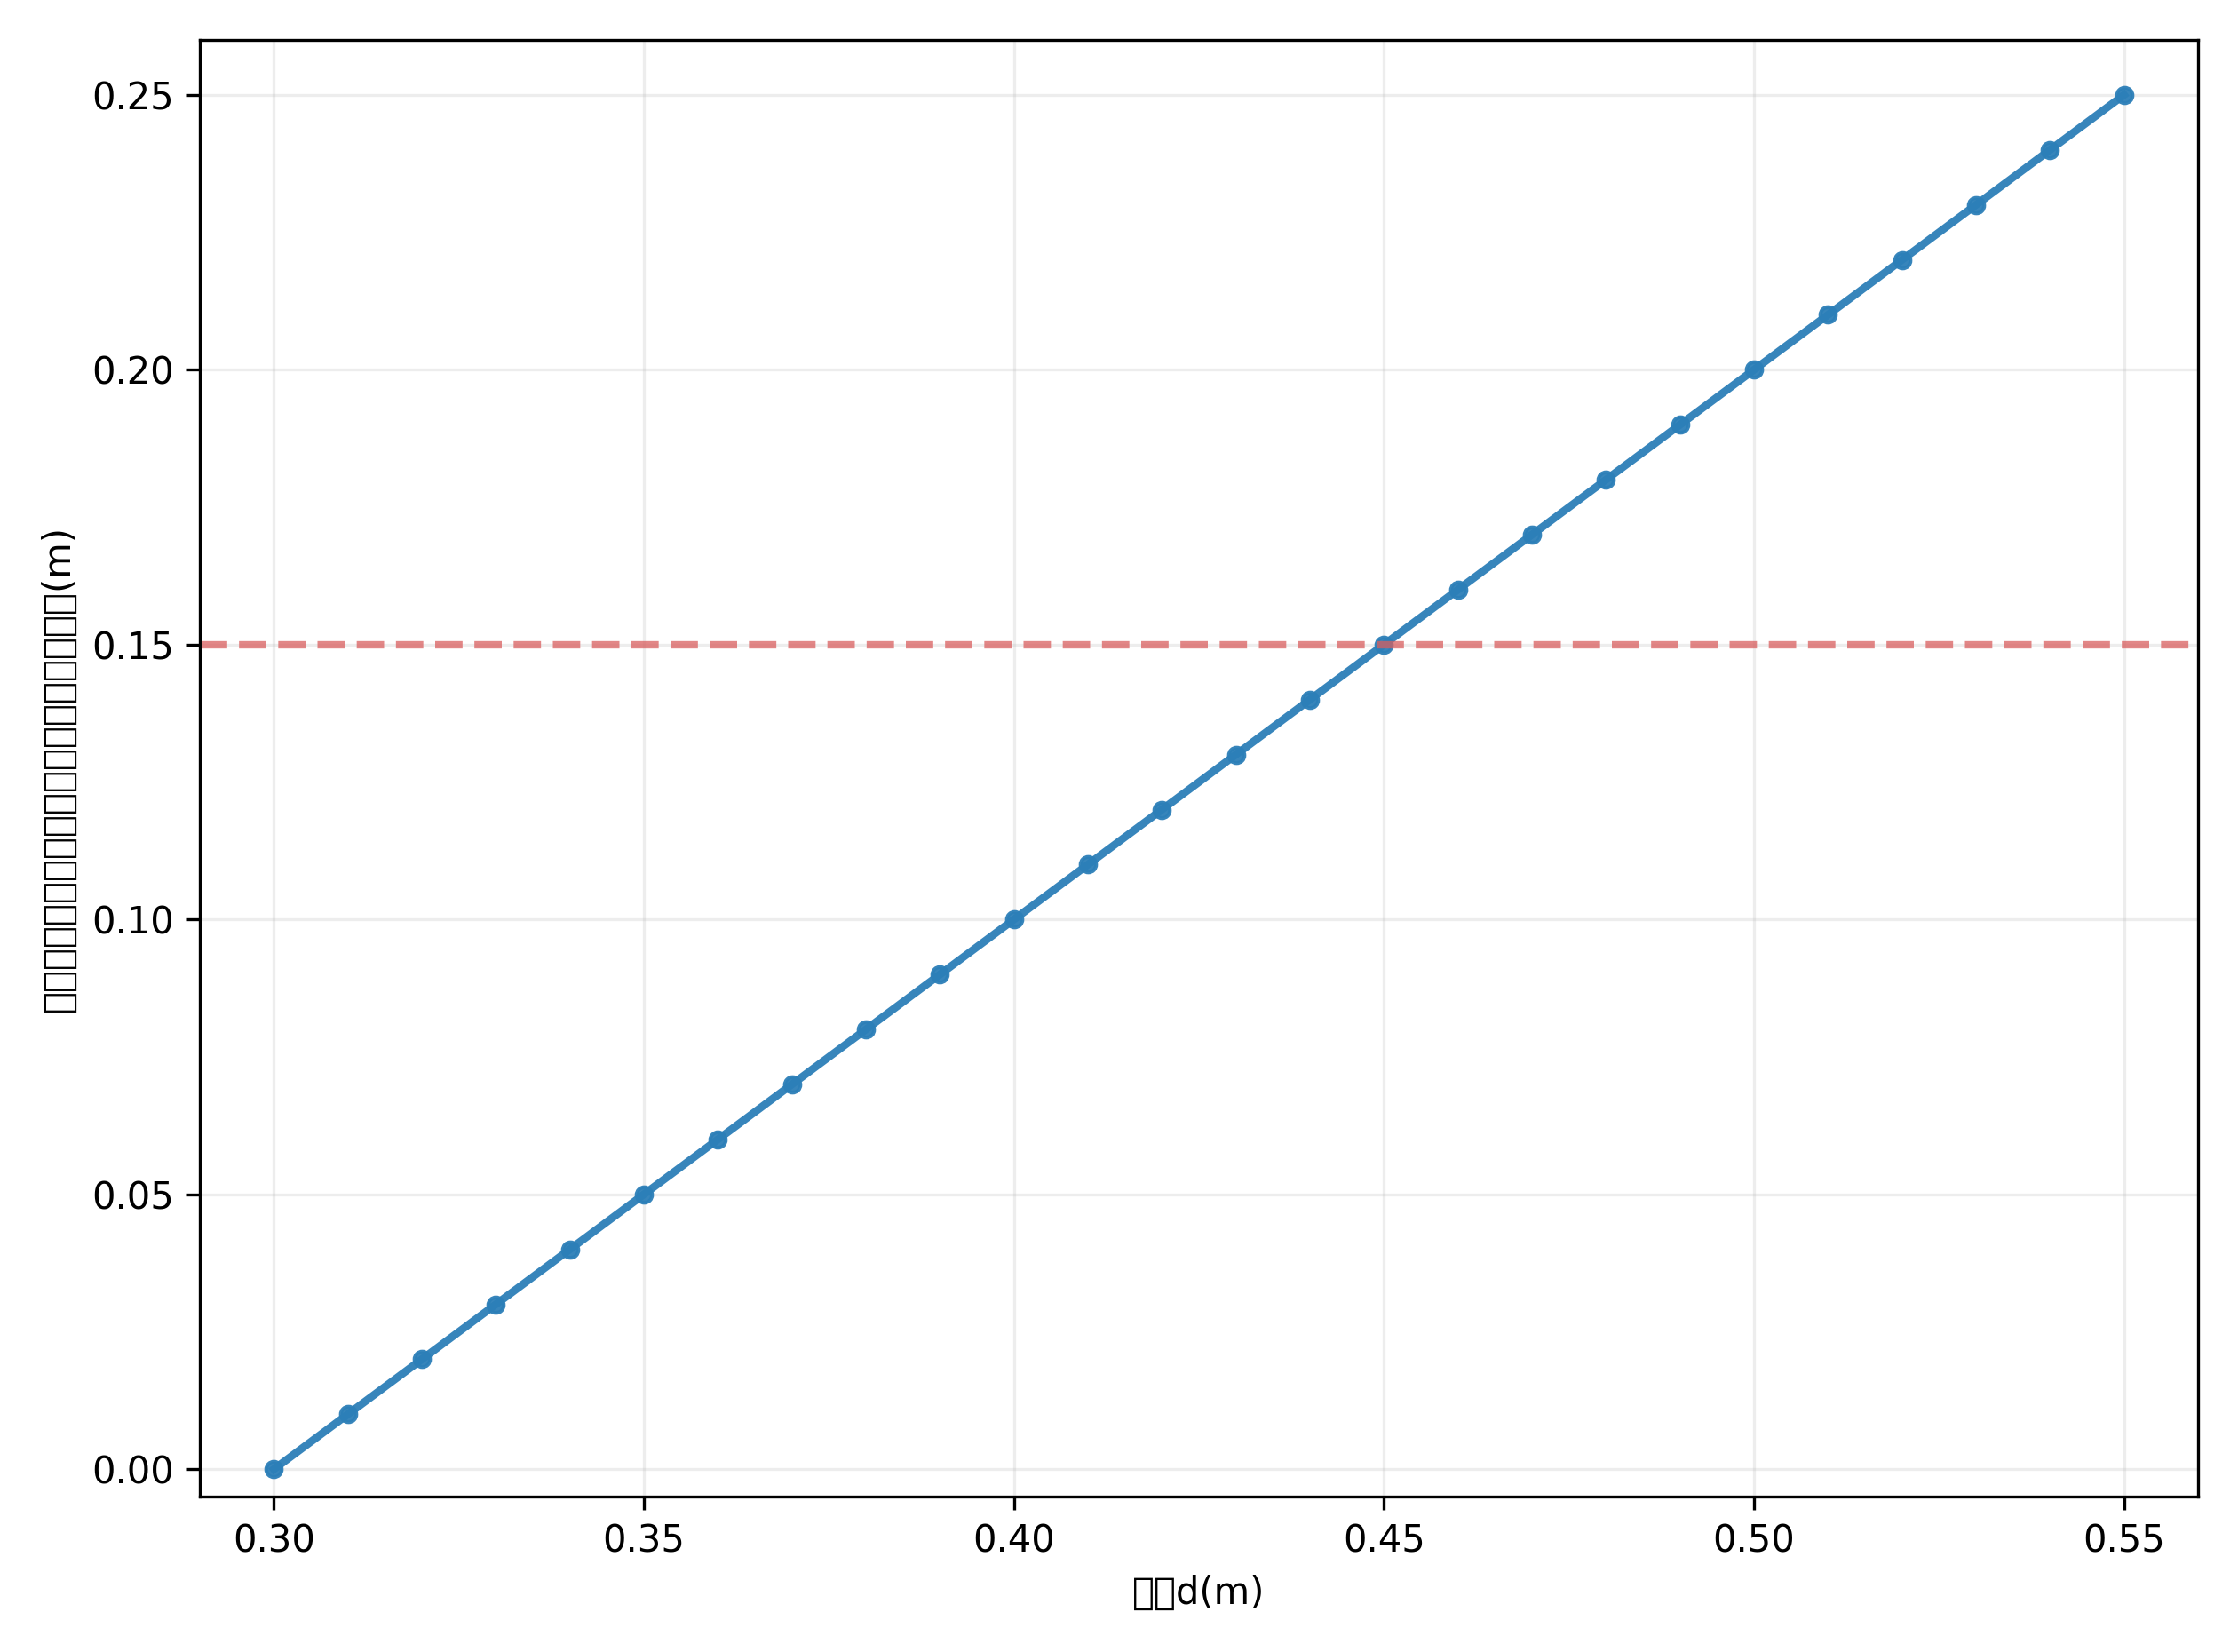
\includegraphics[width=0.80\textwidth]{plot15.png}
\caption{问题三临界螺距附近的最小安全距离关系图}
\label{fig:p3_binary_image}
\end{figure}


\subsection{问题四：调头路径设计与运动仿真}

\subsubsection{问题理解}
问题四要求在给定调头空间约束下，为板凳龙设计一条能够完成转向的连续路径，并在此基础上模拟整条板凳龙在调头阶段的运动状态。与前三问相比，本问的重点不再是单一盘入螺线上的运动，而是需要构造一条由盘入段、调头段和盘出段组成的复合路径，并保证整条路径几何上连续、运动上可实现、过程中不发生碰撞。

从建模角度看，问题四本质上是一个\textbf{受限空间中的组合曲线路径设计与多刚体跟随运动问题}。其核心难点在于：一方面，调头路径必须位于给定调头空间内；另一方面，路径不能过于急剧，否则会导致后续板凳跟随时局部挤压、速度突变或碰撞风险增加。因此，需要在几何连续性、空间可行性与运动安全性之间进行综合平衡。

\subsubsection{模型建立思路}
问题四可以分解为以下四个层次：

\begin{enumerate}
    \item \textbf{路径层：}设计龙头前把手的调头复合路径；
    \item \textbf{连续性层：}保证盘入段、调头段和盘出段之间位置连续，必要时切向连续；
    \item \textbf{跟随层：}利用问题一中的固定把手间距递推模型，求解全队在复合路径上的位置与速度；
    \item \textbf{安全性层：}利用问题二中的碰撞检测方法，验证调头路径下运动过程是否安全。
\end{enumerate}

因此，问题四的建模逻辑可概括为
\[
\text{构造调头路径} \longrightarrow \text{保证几何连续} \longrightarrow \text{全队跟随仿真} \longrightarrow \text{碰撞与速度验证}.
\]

\subsubsection{调头路径的构造思想}
设板凳龙的完整运动过程由三部分组成：

\begin{enumerate}
    \item 盘入路径：龙头前把手沿阿基米德螺线向中心运动；
    \item 调头路径：在有限调头空间内完成方向改变；
    \item 盘出路径：龙头前把手沿与盘入段相衔接的外出路径离开调头区域。
\end{enumerate}

为便于构造平滑路径，本文将调头段设计为由若干圆弧组成的组合曲线。这样做的原因在于：圆弧的参数表达简单，几何意义明确，易于控制曲率和转向角，并且便于与螺线段进行拼接。

设盘入段终点为 $P_{\mathrm{in}}$，盘出段起点为 $P_{\mathrm{out}}$，则调头段的设计目标是在调头空间内构造一条连接这两个点的光滑路径，使得龙头前把手能够由盘入方向连续过渡到盘出方向。

\paragraph{*Python任务1：}
根据给定调头空间半径、盘入终点和盘出起点，编写程序构造调头路径的几何对象，并输出各段曲线的参数表达、关键连接点坐标及圆弧半径等信息。

\subsubsection{盘入段与盘出段的几何表示}
盘入段仍采用阿基米德螺线模型
\begin{equation}
r=\frac{d}{2\pi}\theta,
\end{equation}
其直角坐标表示为
\begin{equation}
x_{\mathrm{in}}(\theta)=\frac{d}{2\pi}\theta\cos\theta,
\qquad
y_{\mathrm{in}}(\theta)=\frac{d}{2\pi}\theta\sin\theta.
\end{equation}

盘出段通常可视为与盘入段具有一定对称关系的外出路径。若采用中心对称构造，则可将盘出段表示为
\begin{equation}
x_{\mathrm{out}}(\theta)=-x_{\mathrm{in}}(\theta),\qquad
y_{\mathrm{out}}(\theta)=-y_{\mathrm{in}}(\theta),
\end{equation}
或者根据实际题意选取与盘入路径相匹配的另一支螺线。无论采用何种构造方式，其基本要求是在调头完成后，龙头前把手能够平稳接入盘出路径。

设盘入段与调头段连接点为 $P_1$，调头段与盘出段连接点为 $P_2$，则路径设计需围绕点 $P_1,P_2$ 进行。

\paragraph{*Python任务2：}
在程序中确定盘入段终点 $P_1$ 与盘出段起点 $P_2$，并计算这两个点处的切向方向，为后续调头圆弧构造提供边界条件。

\subsubsection{调头圆弧段的参数方程}
设调头段由两段圆弧组成，分别记为圆弧 $\Gamma_1$ 与圆弧 $\Gamma_2$。设第一段圆弧圆心为 $O_1=(x_{c1},y_{c1})$，半径为 $R_1$；第二段圆弧圆心为 $O_2=(x_{c2},y_{c2})$，半径为 $R_2$。则其参数方程可写为

\begin{equation}
x_1(\varphi)=x_{c1}+R_1\cos\varphi,\qquad
y_1(\varphi)=y_{c1}+R_1\sin\varphi,
\end{equation}

\begin{equation}
x_2(\psi)=x_{c2}+R_2\cos\psi,\qquad
y_2(\psi)=y_{c2}+R_2\sin\psi.
\end{equation}

其中，参数区间应根据连接点位置和转向方向确定。两段圆弧构成的调头路径应满足以下基本条件：

\begin{enumerate}
    \item $\Gamma_1$ 与盘入段在点 $P_1$ 处连接；
    \item $\Gamma_2$ 与盘出段在点 $P_2$ 处连接；
    \item $\Gamma_1$ 与 $\Gamma_2$ 在中间连接点 $P_m$ 处连续；
    \item 路径整体位于调头空间内部。
\end{enumerate}

若进一步要求路径切向连续，则还需满足
\begin{equation}
\bm{\tau}_{\mathrm{in}}(P_1)=\bm{\tau}_{\Gamma_1}(P_1),
\end{equation}
\begin{equation}
\bm{\tau}_{\Gamma_1}(P_m)=\bm{\tau}_{\Gamma_2}(P_m),
\end{equation}
\begin{equation}
\bm{\tau}_{\Gamma_2}(P_2)=\bm{\tau}_{\mathrm{out}}(P_2),
\end{equation}
其中 $\bm{\tau}$ 表示曲线切向量。

\paragraph{*Python任务3：}
实现两段圆弧调头路径的参数化构造，求解圆心、半径、连接点及参数区间，并验证位置连续性与切向连续性是否成立。

\subsubsection{复合路径的弧长参数化}
为了后续进行速度和位置递推，需要将龙头前把手的完整路径写成统一的弧长参数形式。设复合路径总长度为 $S$，弧长参数记为 $s\in[0,S]$，则龙头前把手在复合路径上的位置可统一表示为
\begin{equation}
\bm{r}(s)=
\begin{cases}
\bm{r}_{\mathrm{in}}(s), & 0\le s<s_1,\\
\bm{r}_{\mathrm{turn}}(s), & s_1\le s<s_2,\\
\bm{r}_{\mathrm{out}}(s), & s_2\le s\le S.
\end{cases}
\end{equation}

若龙头前把手仍保持恒定速度 $v_0$，则有
\begin{equation}
s(t)=v_0 t.
\end{equation}
于是龙头位置关于时间的表达为
\begin{equation}
\bm{r}(t)=\bm{r}(s(t)).
\end{equation}

这种弧长参数化处理的优点在于：不论路径由螺线还是圆弧组成，都可统一为“给定弧长位置、求对应平面坐标”的形式，从而便于后续各把手按照距离约束递推。

\paragraph{*Python任务4：}
对完整复合路径进行离散化与弧长参数化，建立“弧长 $s$—路径坐标 $(x,y)$”之间的映射关系，并实现龙头前把手在任意时刻的位置查询函数。

\subsubsection{全队跟随运动模型}
一旦龙头前把手在复合路径上的位置确定，后续各把手仍可利用问题一中的“相邻把手间距离恒定”条件进行递推。设第 $n$ 个把手在路径上的弧长参数为 $s_n$，则相邻把手满足
\begin{equation}
\|\bm{r}(s_{n+1})-\bm{r}(s_n)\|=l_n,
\end{equation}
其中 $l_n$ 为第 $n$ 个与第 $n+1$ 个把手之间的固定距离。

与问题一不同的是，此时路径不再是单一解析螺线，而是复合离散曲线，因此通常难以直接写出显式递推公式。本文采用数值搜索方法：已知前一个把手在路径上的弧长位置 $s_n$ 后，在其后方搜索满足距离约束的 $s_{n+1}$，从而实现全队位置递推。

当所有把手弧长位置求出后，即可得到对应直角坐标
\begin{equation}
(x_n,y_n)=\bm{r}(s_n).
\end{equation}
进一步，可通过差分法计算速度：
\begin{equation}
v_n(t)\approx
\frac{\sqrt{[x_n(t+\Delta t)-x_n(t)]^2+[y_n(t+\Delta t)-y_n(t)]^2}}{\Delta t}.
\end{equation}

\paragraph{*Python任务5：}
基于复合路径的弧长参数化结果，实现全体把手在调头过程中的位置递推与速度计算，输出指定时刻下龙头、龙身及龙尾的坐标与速度。

\subsubsection{调头过程中的碰撞检测}
调头路径设计完成后，还需验证整条板凳龙在调头阶段是否会发生碰撞。此时可直接复用问题二中的板凳矩形重建与碰撞检测方法。设第 $i$ 节与第 $j$ 节板凳在时刻 $t$ 对应的矩形区域分别为 $\Omega_i(t)$ 与 $\Omega_j(t)$，则若存在
\begin{equation}
\Omega_i(t)\cap\Omega_j(t)\neq\varnothing,
\end{equation}
则认为调头路径在该时刻不可行。

因此，完整调头路径的可行性需同时满足：

\begin{enumerate}
    \item 路径位于调头空间内部；
    \item 全体板凳能够完成跟随；
    \item 调头过程中不发生自碰撞；
    \item 若有速度约束，则各把手速度不超过允许上界。
\end{enumerate}

\paragraph{*Python任务6：}
将问题二中的碰撞检测程序应用于调头阶段，逐时刻检查全队板凳是否发生碰撞，并记录首次碰撞时刻、碰撞板凳编号及对应构型。

\subsubsection{调头路径长度与效果评价}
为了比较不同调头路径设计方案的优劣，还可引入如下评价指标：

\begin{enumerate}
    \item 总路径长度
    \begin{equation}
    S=\int \dif s;
    \end{equation}
    \item 调头段总长度；
    \item 最大曲率或最小转弯半径；
    \item 调头阶段的最大把手速度；
    \item 调头过程中最小安全距离。
\end{enumerate}

一般而言，较短的路径有利于提高效率，但可能导致转弯更加急促，从而增加碰撞风险和速度波动。因此，需要综合比较路径紧凑性与运动安全性。

\paragraph{*Python任务7：}
对所设计调头路径计算总长度、调头段长度、最小安全距离及速度峰值等指标，并绘制调头过程的若干关键时刻构型图，用于评价路径方案的合理性。

\subsubsection{问题四的求解流程}
综上，问题四的求解流程如下：

\begin{enumerate}
    \item 根据盘入段和盘出段的几何关系，确定调头路径的连接边界条件；
    \item 构造由两段圆弧或其他光滑曲线组成的调头段；
    \item 对完整复合路径进行弧长参数化；
    \item 根据固定把手间距，递推求出调头过程中所有把手的位置与速度；
    \item 利用碰撞检测方法验证路径可行性；
    \item 输出调头路径参数、关键时刻构型图及评价指标。
\end{enumerate}

\subsubsection{问题四模型的特点}
本问模型是在前三问基础上的进一步综合，其优点在于：

\begin{itemize}
    \item 将盘入、调头、盘出统一为一条复合路径，便于整体分析；
    \item 圆弧调头模型几何意义清晰，参数较少，易于实现；
    \item 通过弧长参数化处理，能够将不同类型曲线统一纳入一个递推框架；
    \item 可直接与问题二的碰撞检测和问题五的速度约束分析衔接。
\end{itemize}

但该模型也存在一定局限性：

\begin{itemize}
    \item 若调头段仅由少量圆弧构成，可能无法完全反映真实表演中的灵活转向过程；
    \item 全队跟随位置通常依赖数值搜索，计算量较大；
    \item 调头路径的优劣仍受参数选取影响，需要通过数值实验进一步验证。
\end{itemize}

因此，在数值实现中，应适当比较不同调头路径参数下的运动效果，以提高方案的可信度。

\subsubsection{结果输出说明}
完成上述建模与计算后，应给出以下结果：

\begin{enumerate}
    \item 调头路径的几何参数，包括圆心、半径、连接点和总长度；
    \item 龙头前把手在调头过程中的轨迹图；
    \item 若干关键时刻下整条板凳龙的平面构型图；
    \item 调头过程中全体把手的速度变化情况；
    \item 调头路径的碰撞检测结果及最小安全距离。
\end{enumerate}

\noindent 这些结果能够说明在给定调头空间约束下，所设计路径是否能支持板凳龙顺利完成调头，并为后续问题五中的最大允许行进速度分析提供基础。

问题四不仅需要路径图，还需要结合构型与速度进行联合解读。图~\ref{fig:p4_path} 给出了调头路径，图~\ref{fig:p4_configs} 展示起始、中间、结束三个关键构型，图~\ref{fig:p4_speed} 则给出调头阶段速度变化。

\begin{figure}[H]
\centering
\begin{tikzpicture}
\begin{axis}[
    width=0.72\textwidth,
    height=0.48\textwidth,
    xlabel={$x$ / m}, ylabel={$y$ / m},
    title={问题四：调头路径点集},
    grid=both, axis equal image
]
\addplot[orange!85!black,thick,no marks] table[col sep=comma,x=x,y=y] {图片和数据/problem4_fast_path_points.csv};
\end{axis}
\end{tikzpicture}
\caption{问题四调头路径}
\label{fig:p4_path}
\end{figure}

\begin{figure}[H]
    \centering
    \begin{subfigure}[b]{0.31\textwidth}
        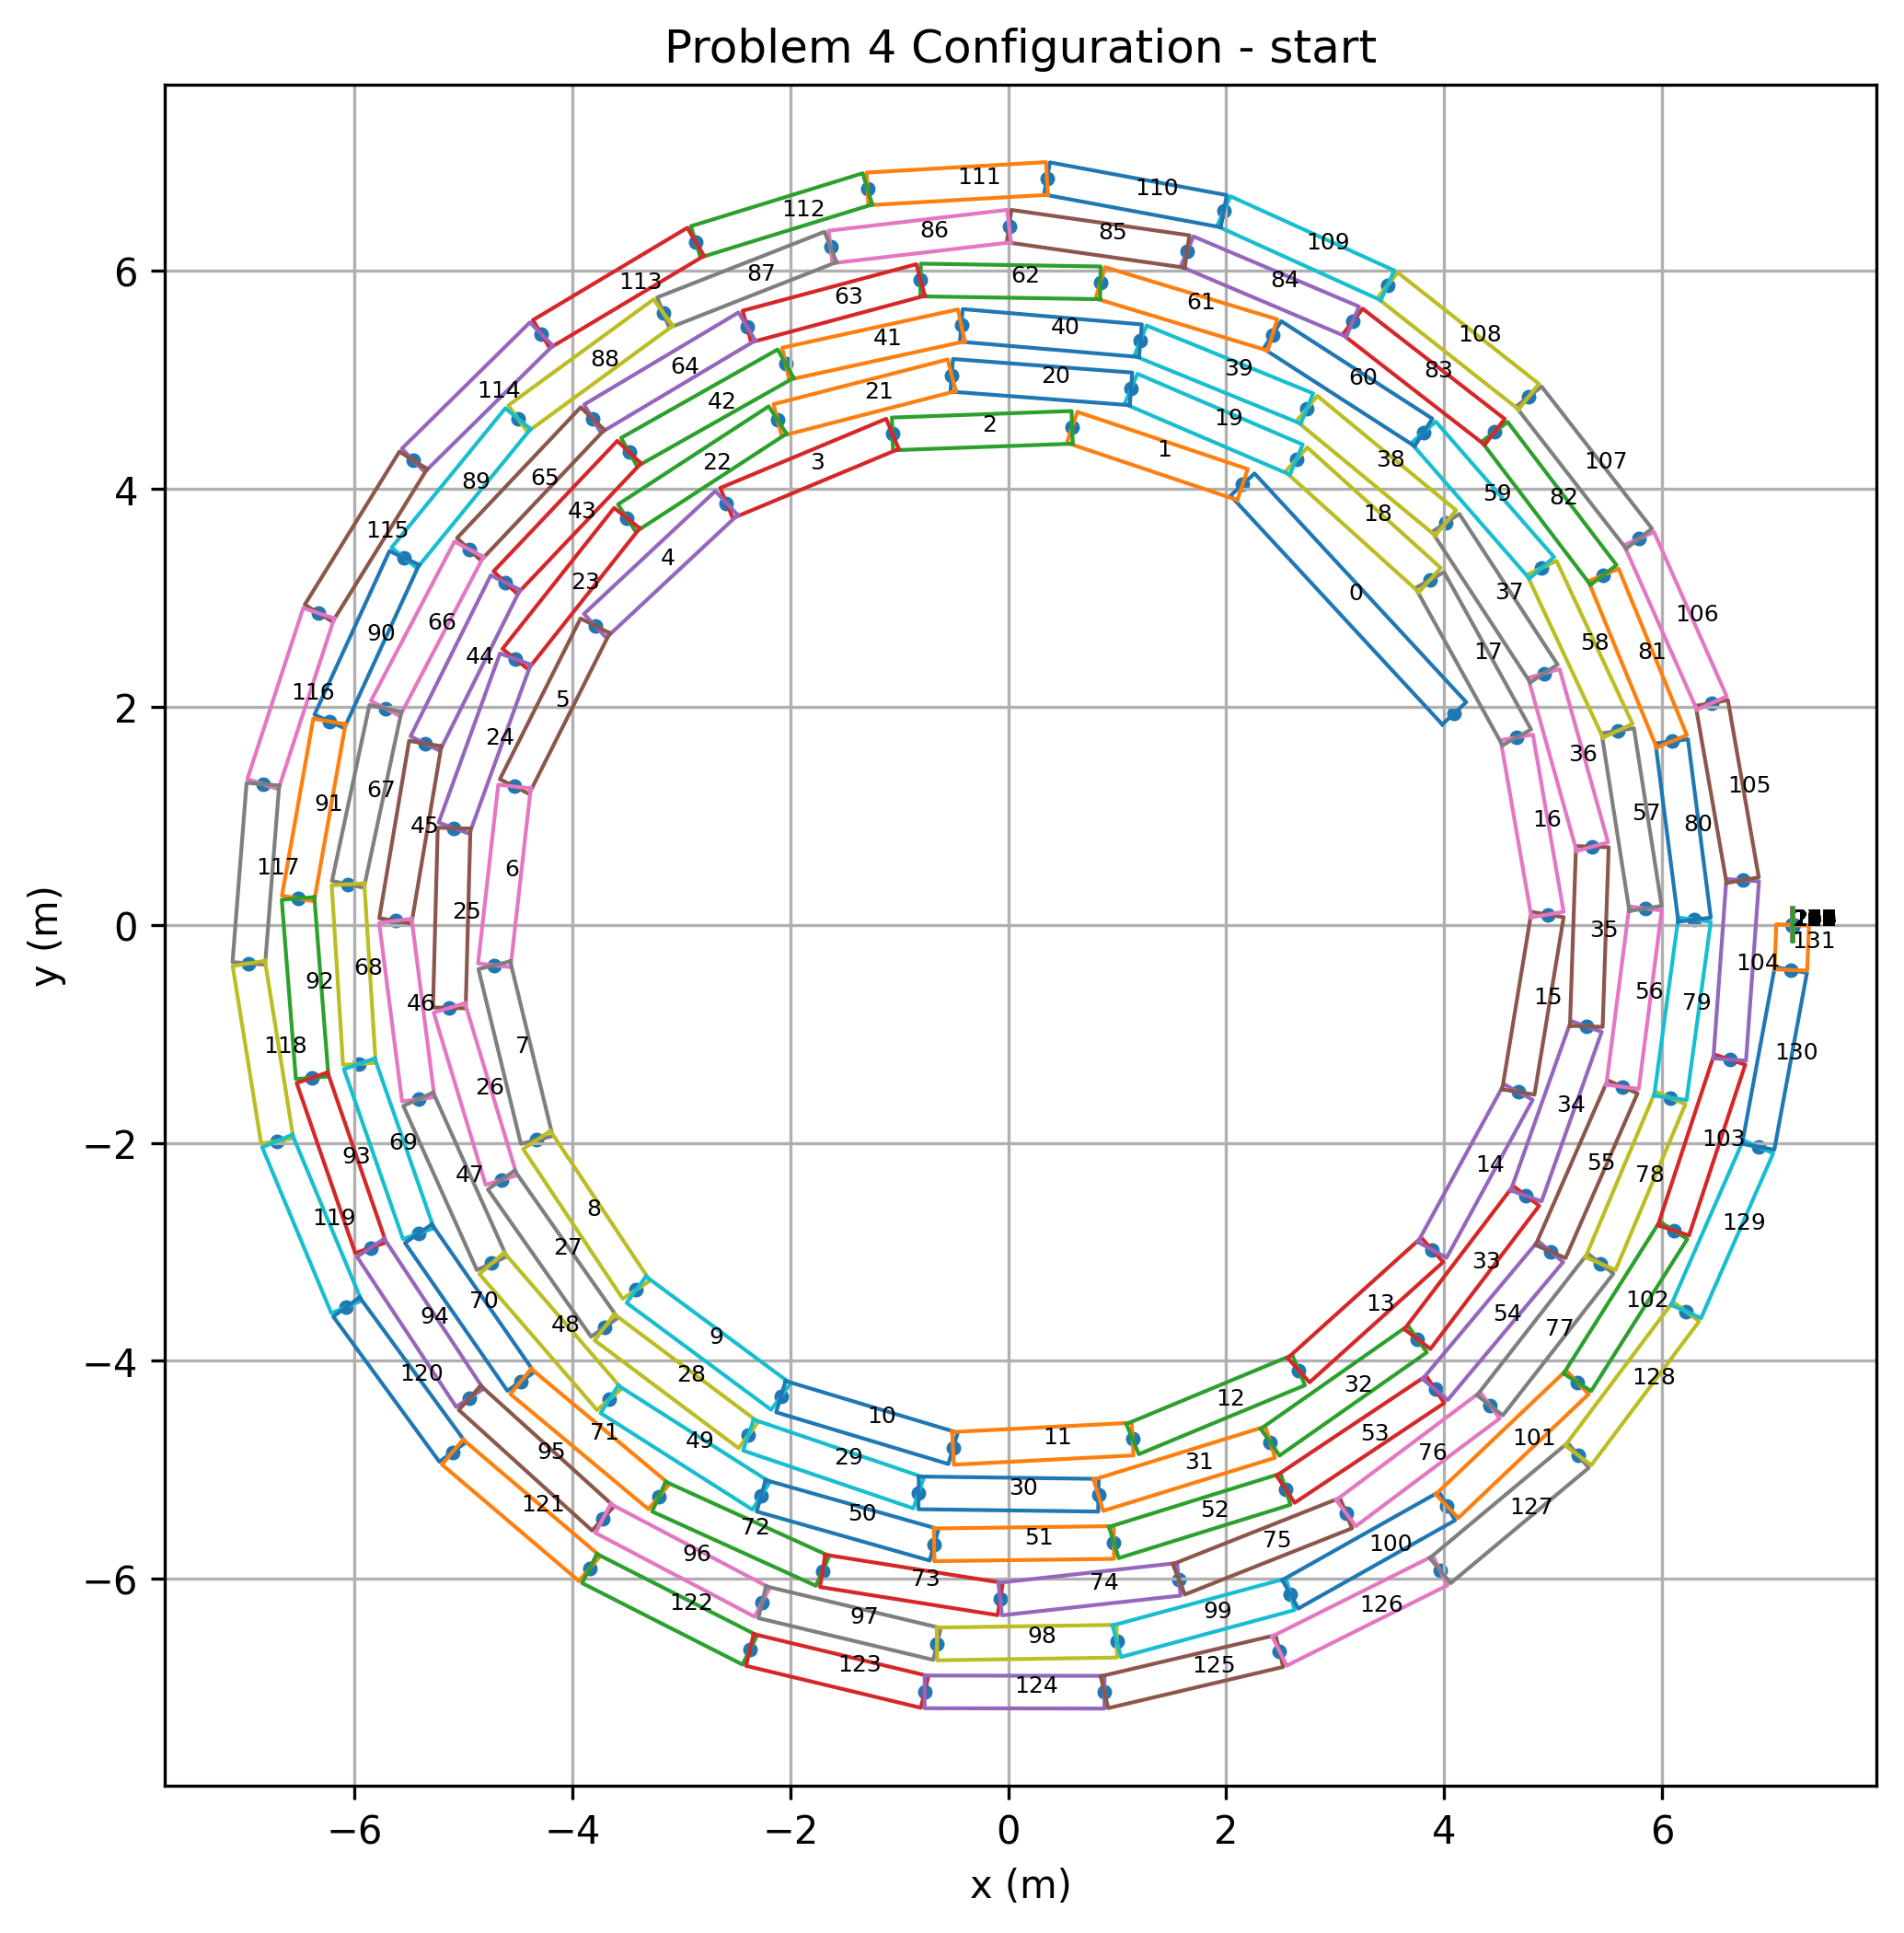
\includegraphics[width=\textwidth]{图片和数据/problem4_fast_config_start.png}
        \caption{起始构型}
    \end{subfigure}
    \hfill
    \begin{subfigure}[b]{0.31\textwidth}
        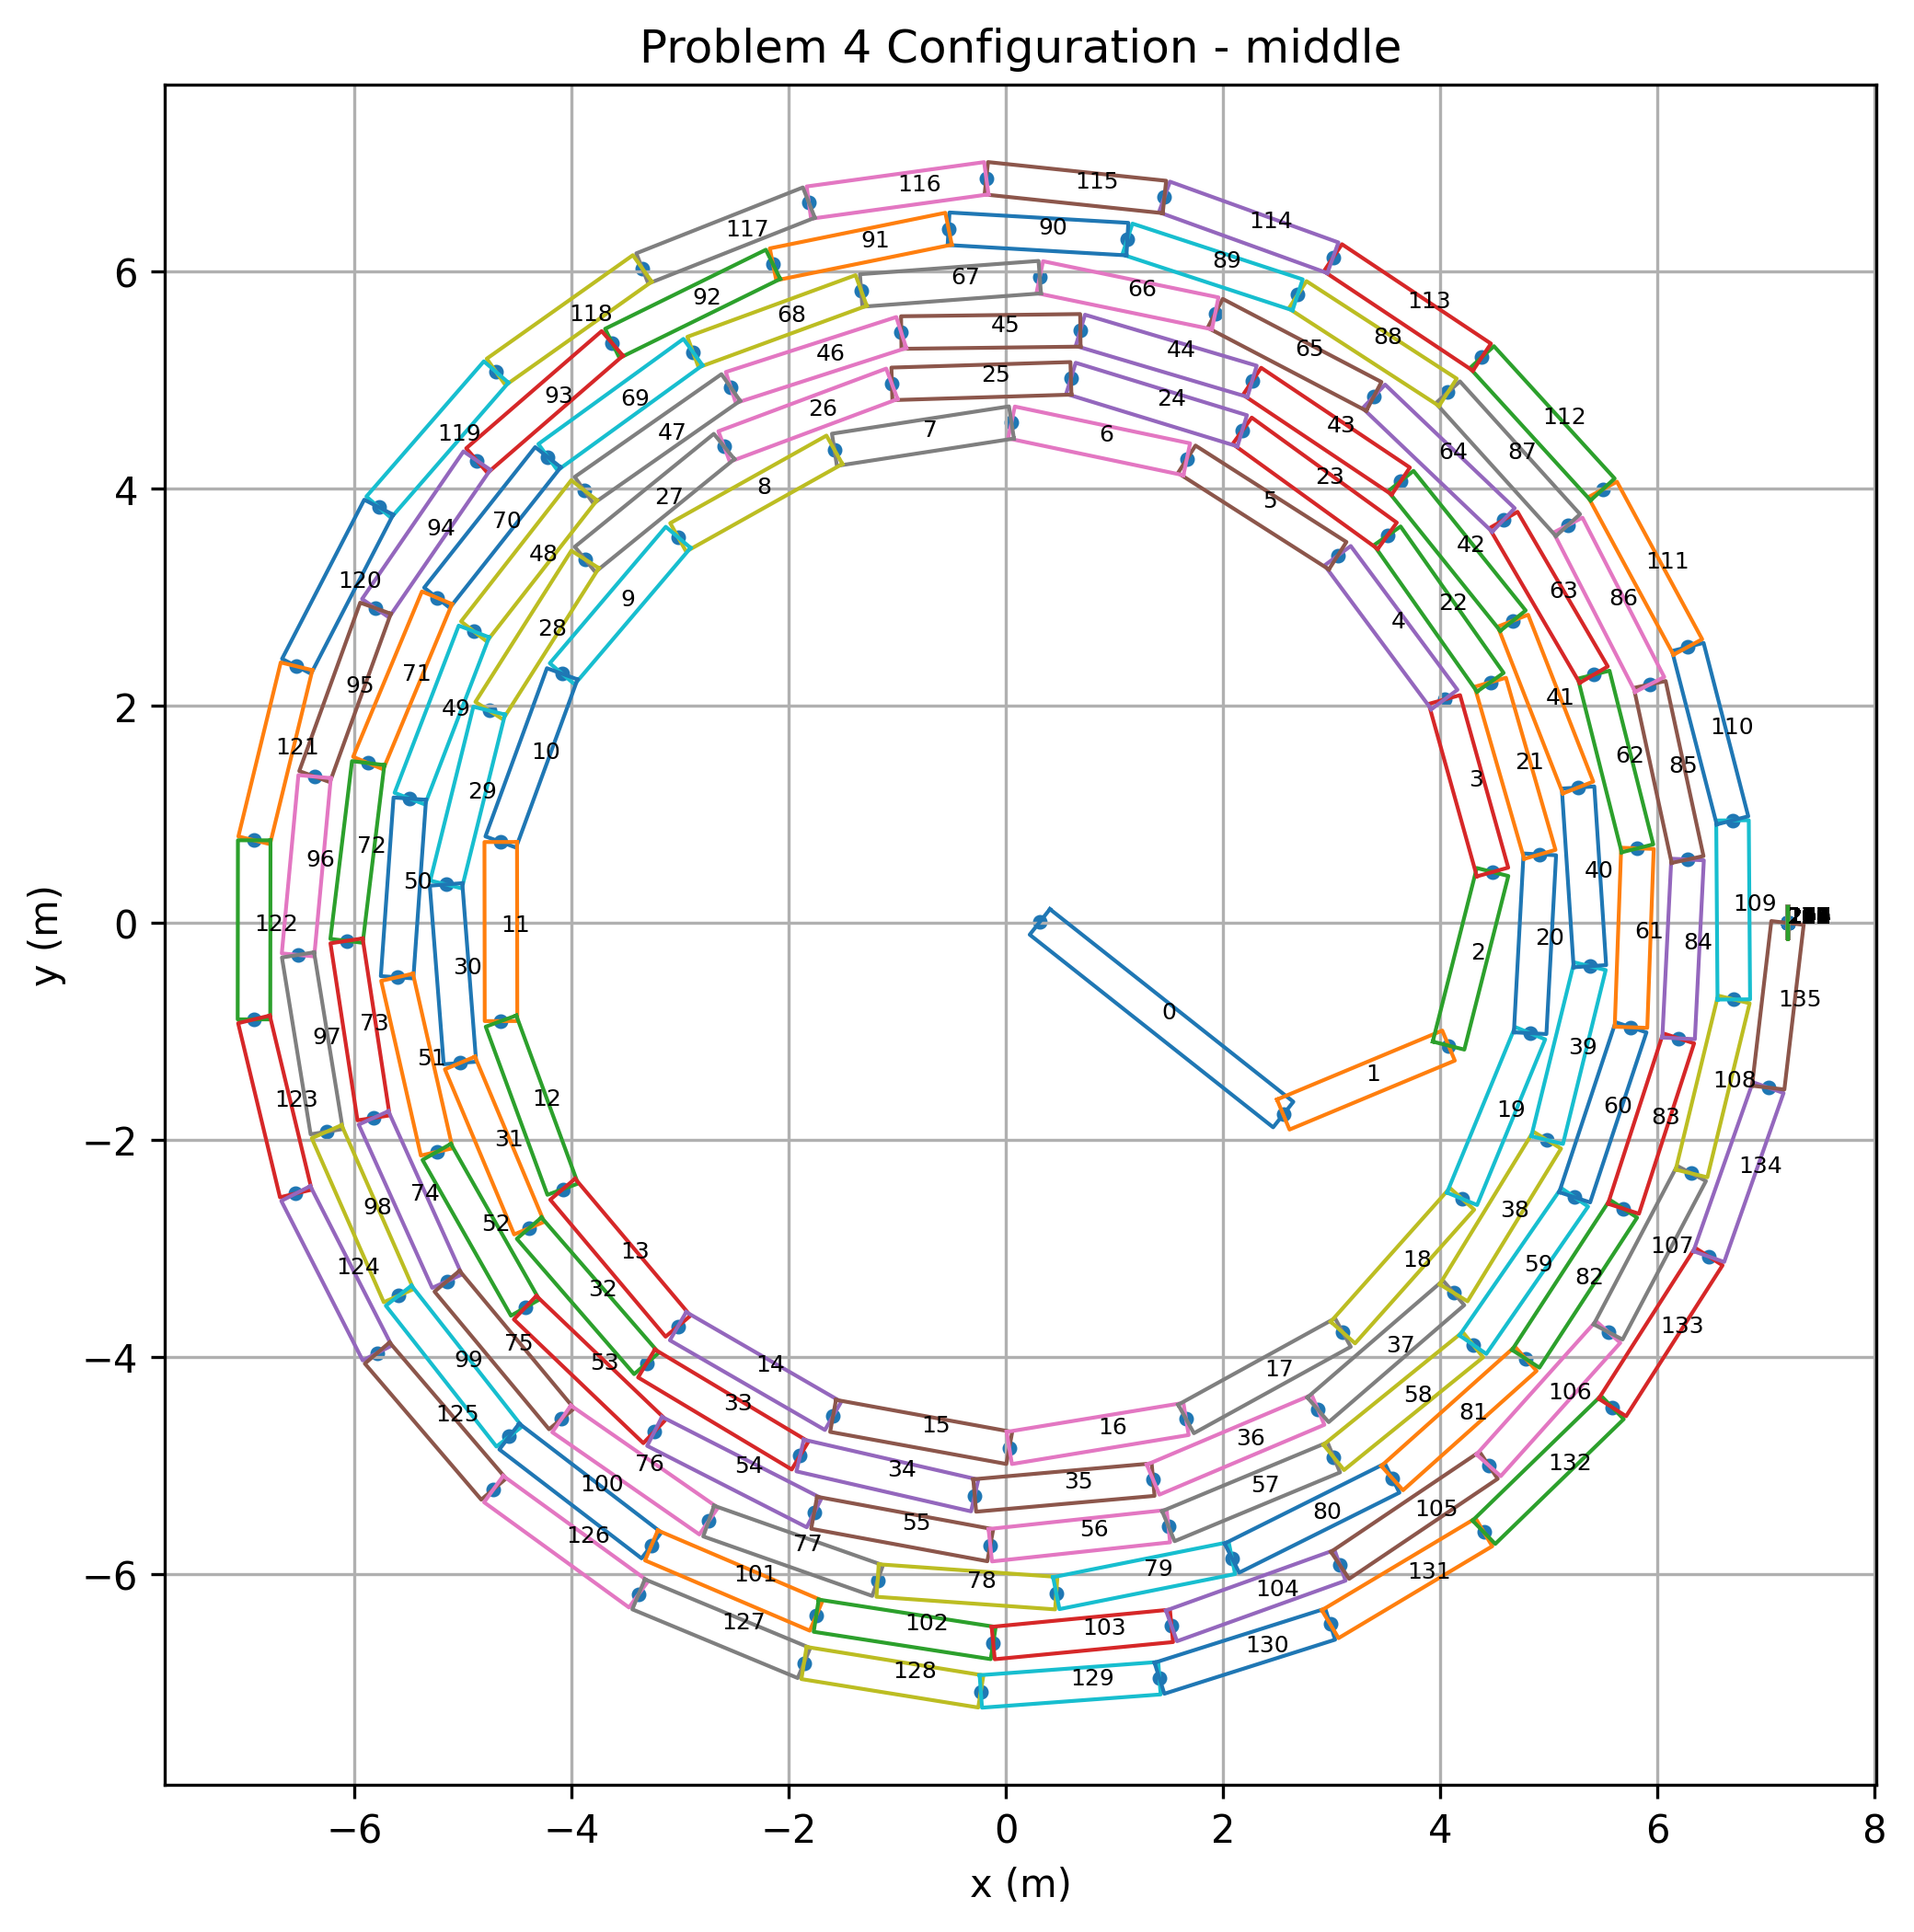
\includegraphics[width=\textwidth]{图片和数据/problem4_fast_config_middle.png}
        \caption{中间构型}
    \end{subfigure}
    \hfill
    \begin{subfigure}[b]{0.31\textwidth}
        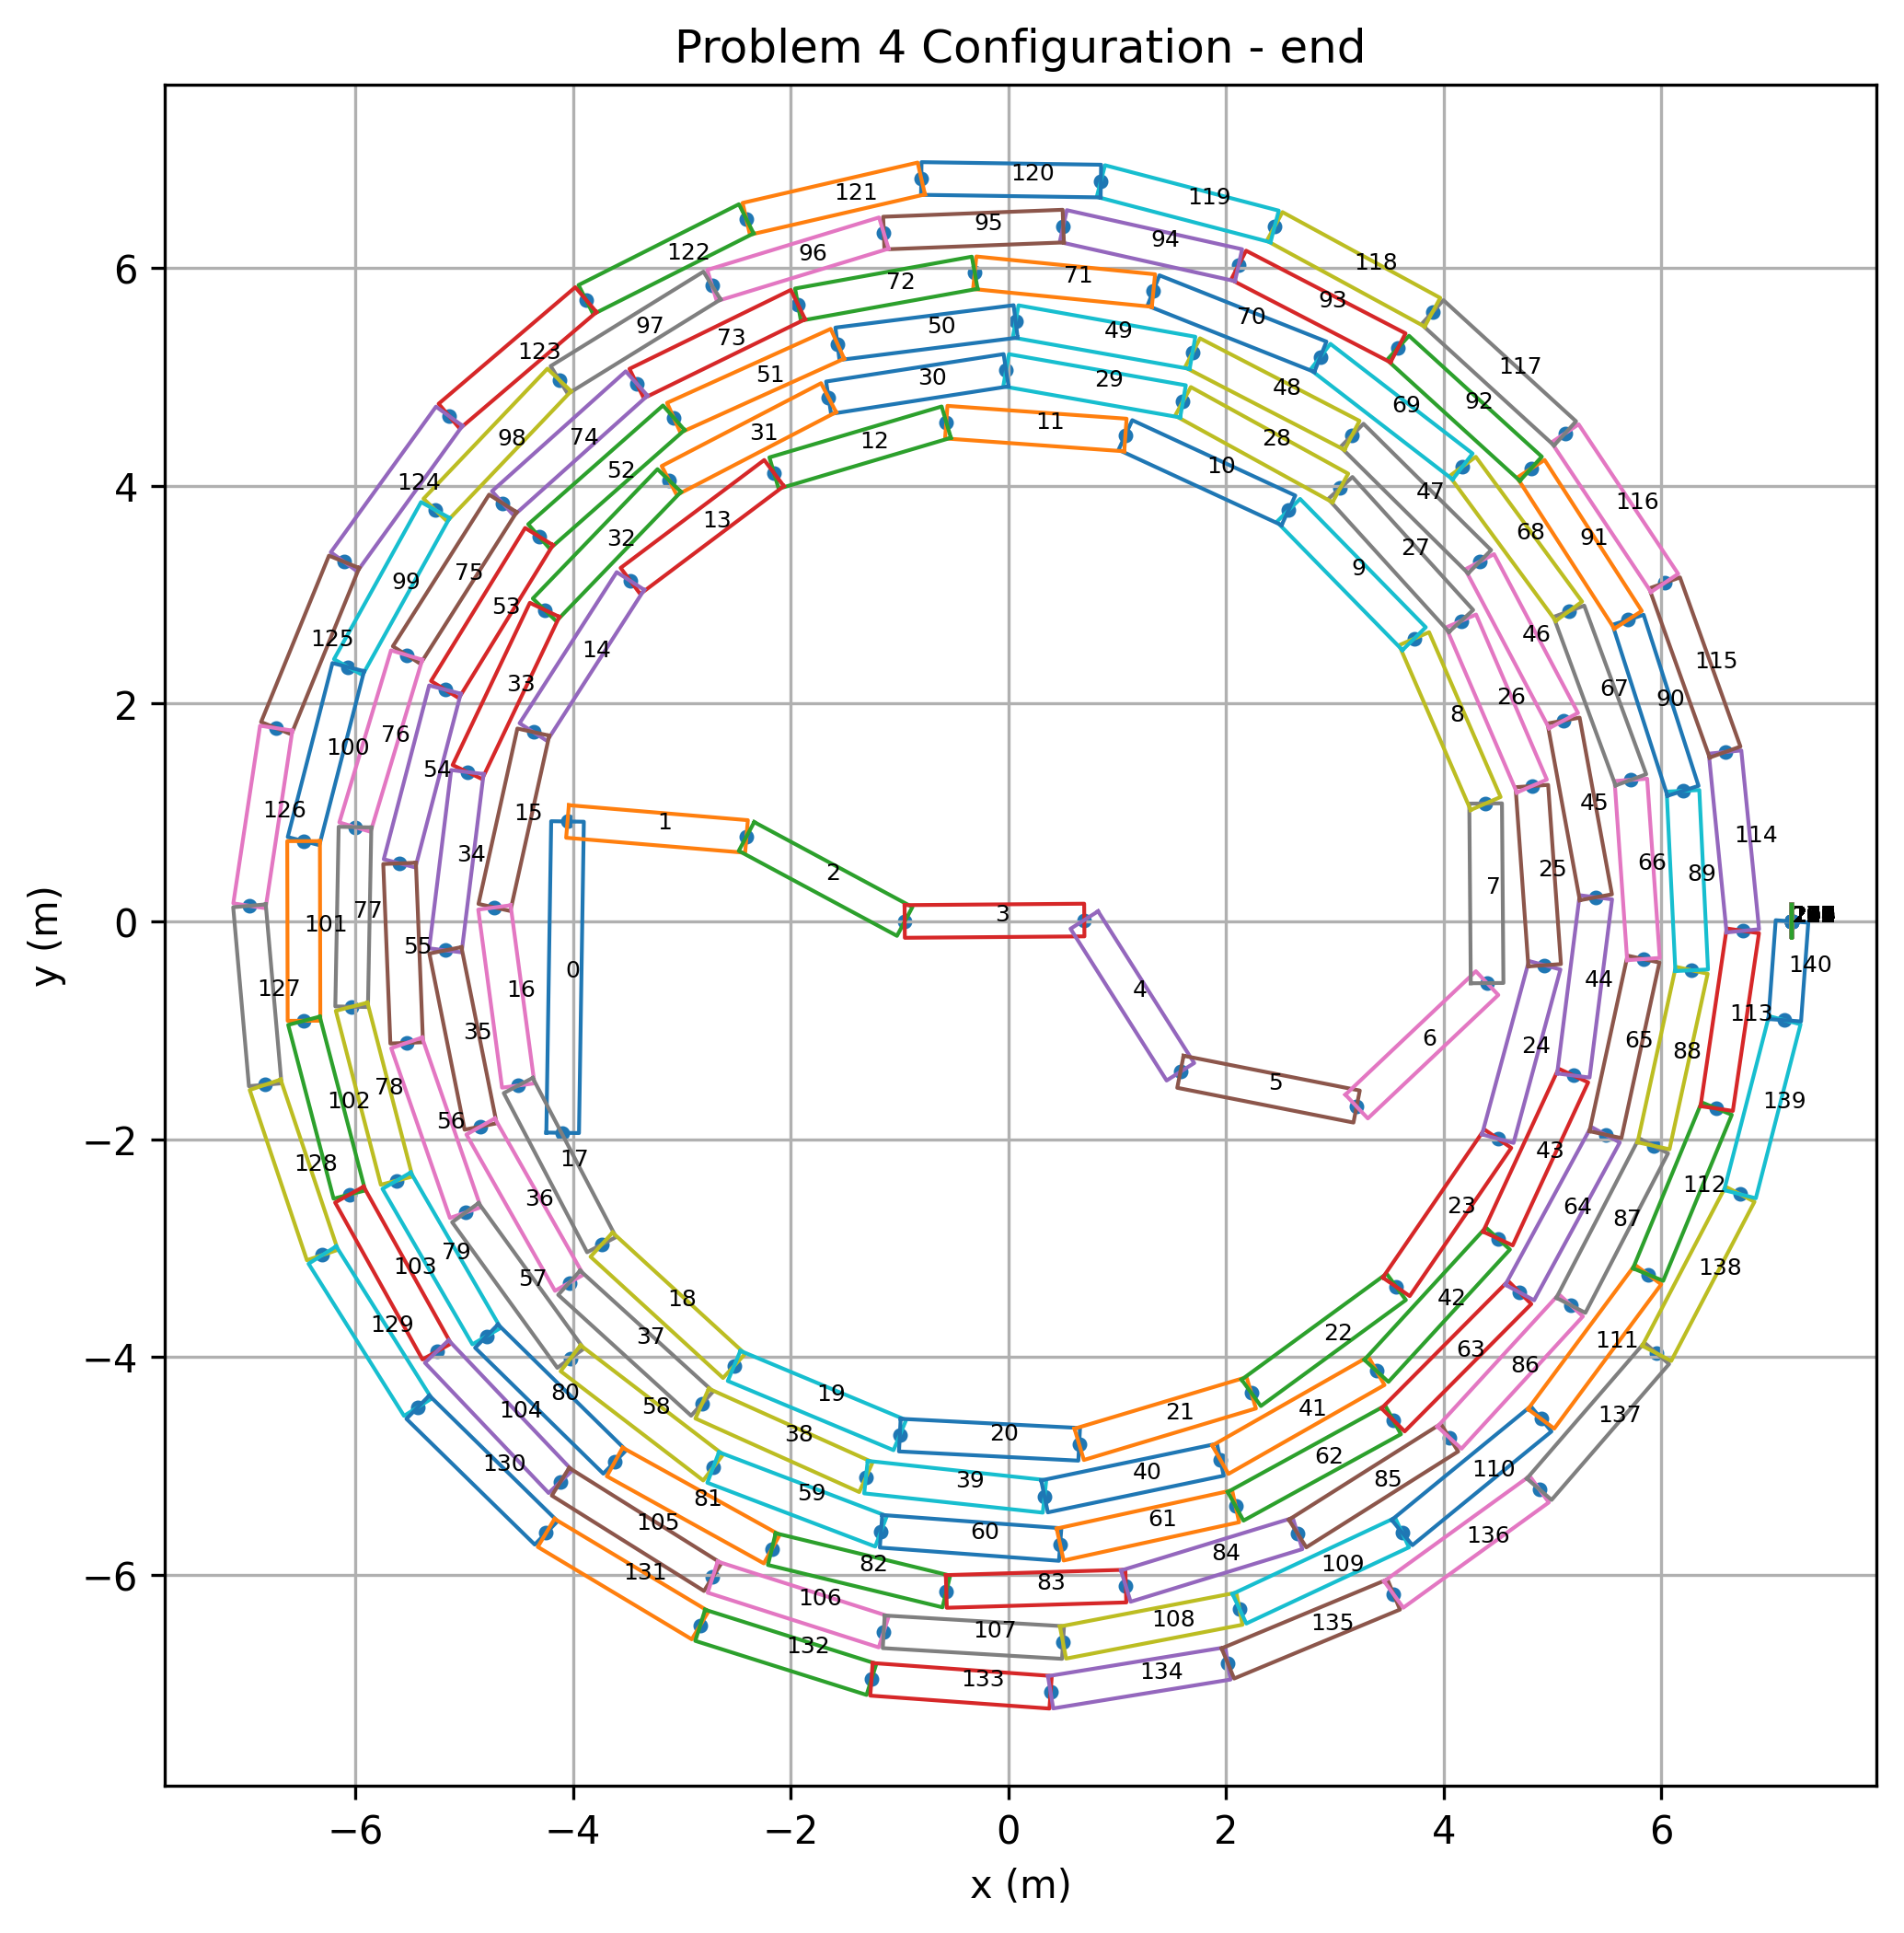
\includegraphics[width=\textwidth]{图片和数据/problem4_fast_config_end.png}
        \caption{结束构型}
    \end{subfigure}
    \caption{问题四关键时刻构型}
    \label{fig:p4_configs}
\end{figure}

\begin{figure}[H]
\centering
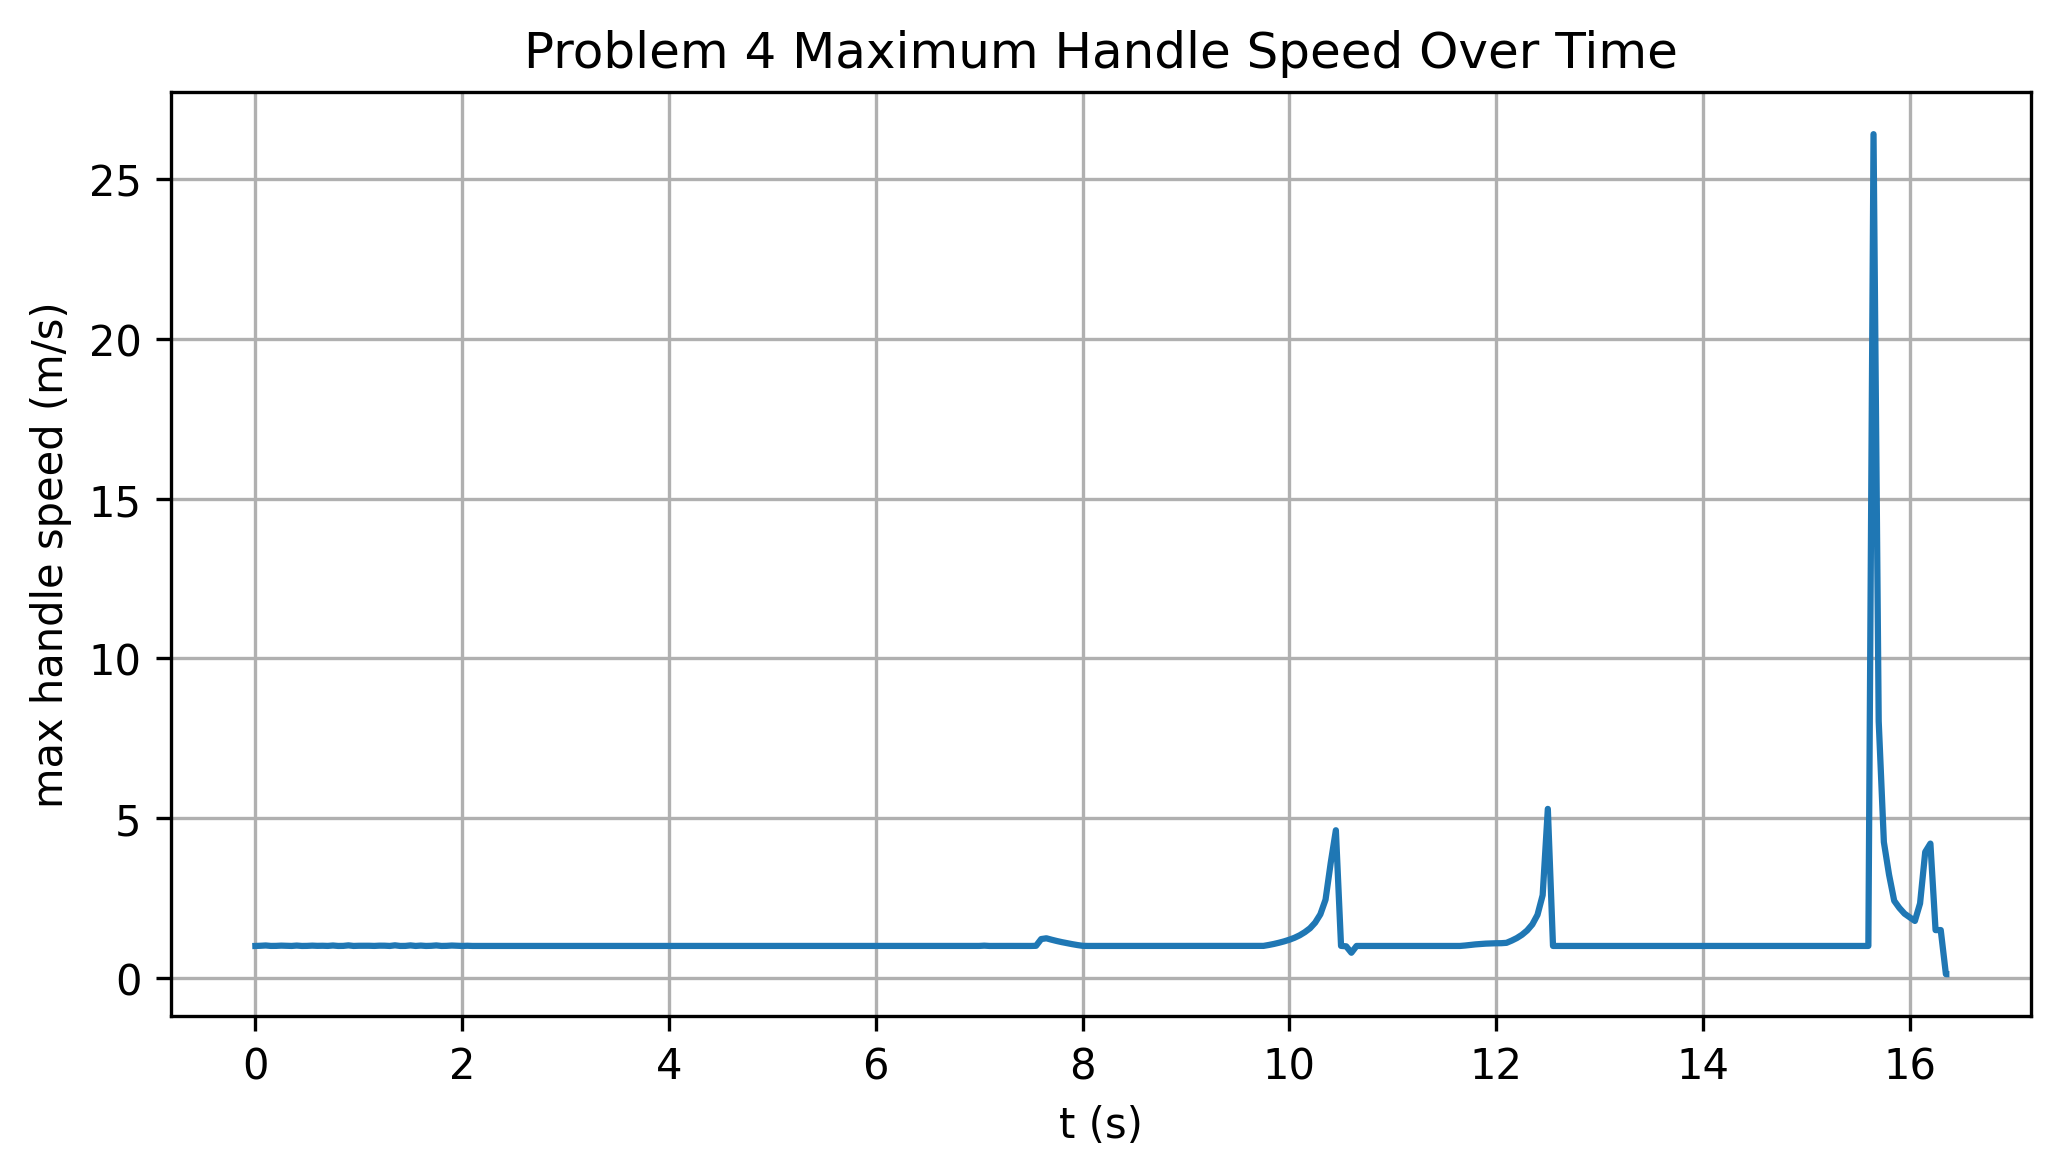
\includegraphics[width=0.75\textwidth]{图片和数据/problem4_fast_speed_curve.png}
\caption{问题四调头阶段速度曲线}
\label{fig:p4_speed}
\end{figure}

为便于对调头阶段的离散结果进行查阅，还可将若干代表性时刻的关键把手坐标与速度整理成表。表~\ref{tab:p4_coords} 汇总了 $t=-100,-50,0,50,100\,\mathrm{s}$ 时龙头、若干代表性龙身以及龙尾后把手的坐标，表~\ref{tab:p4_vels} 给出了同一组时刻下对应的速度结果。

\begin{table}[H]
  \centering
  \caption{调头过程中代表性把手坐标}
  \label{tab:p4_coords}
  \resizebox{\textwidth}{!}{%
  \begin{tabular}{lrrrrr}
    \toprule
    \textbf{把手/板凳} & \textbf{$t=-100$ s} & \textbf{$t=-50$ s} & \textbf{$t=0$ s} & \textbf{$t=50$ s} & \textbf{$t=100$ s} \\
    \midrule
    龙头 $x$ (m)        &  7.778034 &  6.608301 & -2.711856 &  1.332696 & -3.157229 \\
    龙头 $y$ (m)        &  3.717164 &  1.898865 & -3.591078 &  6.175324 &  7.548511 \\
    \midrule
    第 1 节龙身 $x$ (m)          &  6.209273 &  5.366911 & -0.063534 &  3.862265 & -0.346890 \\
    第 1 节龙身 $y$ (m)          &  6.108521 &  4.475403 & -4.670888 &  4.840828 &  8.079166 \\
    \midrule
    第 51 节龙身 $x$ (m)         & -10.608038 & -3.629945 &  2.459962 & -1.671385 &  2.095033 \\
    第 51 节龙身 $y$ (m)         &  2.831491 & -8.963800 & -7.778145 & -6.076713 &  4.033787 \\
    \midrule
    第 101 节龙身 $x$ (m)        & -11.922761 & 10.125787 &  3.008493 & -7.591816 & -7.288774 \\
    第 101 节龙身 $y$ (m)        & -4.802378 & -5.972247 & 10.108539 &  5.175487 &  2.063875 \\
    \midrule
    第 151 节龙身 $x$ (m)        & -14.351032 & 12.974784 & -7.002789 & -4.605165 &  9.462513 \\
    第 151 节龙身 $y$ (m)        & -1.980993 & -3.810357 & 10.337482 & -10.386988 & -3.540357 \\
    \midrule
    第 201 节龙身 $x$ (m)        & -11.952942 & 10.522508 & -6.872842 &  0.336952 &  8.524374 \\
    第 201 节龙身 $y$ (m)        & 10.566998 & -10.807425 & 12.382609 & -13.177610 &  8.606933 \\
    \midrule
    龙尾（后） $x$ (m) & -1.011059 &  0.189809 & -1.933627 &  5.859094 & -10.980157 \\
    龙尾（后） $y$ (m) & -16.527573 & 15.720588 & -14.713128 & 12.612894 & -6.770006 \\
    \bottomrule
  \end{tabular}%
  }
\end{table}

\begin{table}[H]
  \centering
  \caption{调头过程中代表性把手速度}
  \label{tab:p4_vels}
  \resizebox{0.88\textwidth}{!}{%
  \begin{tabular}{lrrrrr}
    \toprule
    \textbf{把手/板凳} & \textbf{$t=-100$ s} & \textbf{$t=-50$ s} & \textbf{$t=0$ s} & \textbf{$t=50$ s} & \textbf{$t=100$ s} \\
    \midrule
    龙头 (m/s)         & 1.000000 & 1.000000 & 1.000000 & 1.000000 & 1.000000 \\
    第 1 节龙身 (m/s)  & 0.999904 & 0.999762 & 0.998687 & 1.000363 & 1.000124 \\
    第 51 节龙身 (m/s) & 0.999346 & 0.998642 & 0.995134 & 0.949935 & 1.003966 \\
    第 101 节龙身 (m/s) & 0.999091 & 0.998248 & 0.994448 & 0.948482 & 1.096263 \\
    第 151 节龙身 (m/s) & 0.998944 & 0.998047 & 0.994156 & 0.948038 & 1.095306 \\
    第 201 节龙身 (m/s) & 0.998849 & 0.997925 & 0.993994 & 0.947823 & 1.094933 \\
    龙尾（后） (m/s)   & 0.998817 & 0.997885 & 0.993944 & 0.947760 & 1.094833 \\
    \bottomrule
  \end{tabular}%
  }
\end{table}


\subsection{问题五：最大允许行进速度分析}

\subsubsection{问题理解}
问题五要求在给定各板凳速度上限约束的条件下，确定龙头前把手允许的最大行进速度。与前四问相比，本问不再主要关注路径构造或碰撞判定，而是研究当龙头以不同速度运动时，整条板凳龙中各把手速度如何被放大，以及这种放大效应对系统整体运行安全性的限制。

从建模角度看，问题五本质上是一个\textbf{带全局速度约束的参数优化问题}。龙头前把手作为主动驱动点，其速度会通过路径曲率变化与刚体链式约束传递到后续板凳。尤其在盘入、调头等曲率较大的区域，后续板凳的速度往往会出现局部放大现象。因此，需要找出在整条路径和整个运动过程中，使所有把手速度都不超过给定阈值的龙头最大允许速度。

\subsubsection{模型建立思路}
问题五可以分解为以下三个层次：

\begin{enumerate}
    \item \textbf{驱动层：}设定龙头前把手行进速度 $v_0$；
    \item \textbf{响应层：}在已知路径和跟随模型下，计算整条板凳龙所有把手的速度分布；
    \item \textbf{优化层：}在满足所有把手速度均不超过阈值的条件下，求解最大允许的 $v_0$。
\end{enumerate}

因此，问题五的建模逻辑可概括为
\[
\text{给定龙头速度 } v_0 \longrightarrow \text{全队速度仿真} \longrightarrow \text{判定是否超速} \longrightarrow \max v_0.
\]

\subsubsection{速度约束的数学表述}
设第 $n$ 个把手在时刻 $t$ 的速度为 $v_n(t)$，题目给定所有把手的速度上限为
\begin{equation}
v_{\mathrm{lim}}.
\end{equation}
则要求对任意把手、任意时刻均满足
\begin{equation}
v_n(t)\le v_{\mathrm{lim}}, \qquad \forall n,\ \forall t.
\end{equation}

记全体把手在全过程中的最大速度为
\begin{equation}
V_{\max}(v_0)=\max_{n,t} v_n(t),
\end{equation}
则问题五等价于求解
\begin{equation}
\max v_0
\end{equation}
满足
\begin{equation}
V_{\max}(v_0)\le v_{\mathrm{lim}}.
\end{equation}

也就是说，只要能够建立“龙头速度 $v_0$ 与全队最大速度 $V_{\max}$”之间的映射关系，便可将问题五转化为单变量约束优化问题。

\paragraph{*Python任务1：}
在问题一或问题四已建立的运动仿真框架基础上，将龙头速度 $v_0$ 设置为可调参数，并在给定 $v_0$ 时输出全体把手在全过程中的速度矩阵以及全局最大速度
\[
V_{\max}(v_0)=\max_{n,t} v_n(t).
\]

\subsubsection{龙头速度与全队速度的关系}
在前述模型中，龙头前把手沿给定路径运动。若路径已按弧长参数 $s$ 表示，则有
\begin{equation}
s(t)=v_0 t.
\end{equation}
因此，龙头前把手的空间位置为
\begin{equation}
\bm{r}_0(t)=\bm{r}(s(t)).
\end{equation}

由于其余把手通过固定距离约束依次跟随龙头运动，因此整个系统的速度场最终由路径几何特征和龙头速度共同决定。一般来说，在路径形状固定时，各把手速度与龙头速度近似成比例关系，即存在某种放大系数 $\lambda_n(t)$，使得
\begin{equation}
v_n(t)\approx \lambda_n(t)\,v_0.
\end{equation}
从而有
\begin{equation}
V_{\max}(v_0)\approx \Lambda_{\max}\,v_0,
\end{equation}
其中
\begin{equation}
\Lambda_{\max}=\max_{n,t}\lambda_n(t).
\end{equation}

这说明：在路径固定的前提下，问题五通常具有较好的单调性，即龙头速度越大，全队最大速度也越大。因此可以采用扫描或二分搜索来求最大允许龙头速度。

\paragraph{*Python任务2：}
选取若干组龙头速度 $v_0$ 进行数值实验，计算对应的全队最大速度 $V_{\max}(v_0)$，绘制“龙头速度—全队最大速度”关系曲线，以验证单调性并估计速度放大倍数。

\subsubsection{速度计算方法}
已知第 $n$ 个把手在离散时刻 $t_k$ 的位置为
\[
(x_n(t_k),y_n(t_k)),
\]
则可用差分法近似其速度：
\begin{equation}
v_n(t_k)\approx
\frac{\sqrt{[x_n(t_{k+1})-x_n(t_k)]^2+[y_n(t_{k+1})-y_n(t_k)]^2}}{\Delta t}.
\end{equation}

若路径与位置递推精度较高，则该方法能够较好地逼近真实瞬时速度。由此可求出全部把手在全部离散时刻的速度矩阵
\begin{equation}
\bm{V}=\bigl(v_n(t_k)\bigr).
\end{equation}
进一步地，定义
\begin{equation}
V_{\max}(v_0)=\max_{n,k} v_n(t_k),
\end{equation}
并记达到该最大值的把手编号和时刻为
\begin{equation}
(n^\ast,t^\ast)=\arg\max_{n,k} v_n(t_k).
\end{equation}

这两个量对于问题五十分重要，因为它们不仅决定了速度约束是否被触发，也能够揭示系统中最容易超速的部位和最危险的时刻。

\paragraph{*Python任务3：}
对每组给定龙头速度 $v_0$，输出全局最大速度 $V_{\max}(v_0)$、达到最大值的把手编号 $n^\ast$ 和对应时刻 $t^\ast$，并记录该把手在该时刻的空间位置。

\subsubsection{最大允许速度优化模型}
设可行性判定函数为
\begin{equation}
G(v_0)=
\begin{cases}
1, & \text{若 } V_{\max}(v_0)\le v_{\mathrm{lim}},\\
0, & \text{若 } V_{\max}(v_0)>v_{\mathrm{lim}}.
\end{cases}
\end{equation}
则问题五可形式化为
\begin{equation}
\max v_0
\end{equation}
满足
\begin{equation}
G(v_0)=1.
\end{equation}

由于 $G(v_0)$ 通常关于 $v_0$ 具有单调性，因此可采用如下数值方法：

\begin{itemize}
    \item 先进行粗扫描，找到“可行—不可行”之间的大致区间；
    \item 再在该区间内使用二分搜索，逼近最大允许龙头速度。
\end{itemize}

设初始搜索区间为
\begin{equation}
[v_L,v_R],
\end{equation}
其中 $v_L$ 为可行速度，$v_R$ 为不可行速度。取中点
\begin{equation}
v_M=\frac{v_L+v_R}{2},
\end{equation}
若 $G(v_M)=1$，则令 $v_L=v_M$；否则令 $v_R=v_M$。重复该过程，直到
\begin{equation}
v_R-v_L<\varepsilon_v,
\end{equation}
其中 $\varepsilon_v$ 为速度搜索精度。最终取
\begin{equation}
v_0^\ast\approx v_L
\end{equation}
作为龙头最大允许行进速度的数值近似。

\paragraph{*Python任务4：}
实现龙头速度的粗扫描与二分搜索算法，求解满足全体把手速度不超过上限 $v_{\mathrm{lim}}$ 时的最大允许龙头速度 $v_0^\ast$。

\subsubsection{关键超速位置分析}
在求得最大允许龙头速度后，还需进一步分析哪些把手最容易成为速度瓶颈。设在最优速度 $v_0^\ast$ 下，全体把手速度矩阵为 $\bm{V}^\ast$，其最大值为
\begin{equation}
V_{\max}(v_0^\ast)=\max_{n,t} v_n(t).
\end{equation}
若该值接近约束上限 $v_{\mathrm{lim}}$，则达到最大值的把手和时刻就对应系统的“临界超速位置”。

通过分析这些临界位置，可以回答以下问题：

\begin{enumerate}
    \item 是龙头、龙身还是龙尾更容易首先达到速度上限；
    \item 速度峰值更容易出现在盘入阶段、调头阶段还是盘出阶段；
    \item 路径曲率较大的区域是否会显著放大局部速度。
\end{enumerate}

这些分析不仅有助于解释最大允许速度的形成机制，也可以为进一步优化路径设计提供参考。

\paragraph{*Python任务5：}
在最优龙头速度 $v_0^\ast$ 下，统计速度最大的若干把手及对应时刻，绘制关键把手速度曲线和速度峰值出现位置图，并判断速度瓶颈主要出现在盘入段、调头段还是盘出段。

\subsubsection{敏感性分析}
为考察结果的稳健性，可对速度上限 $v_{\mathrm{lim}}$ 或路径几何参数进行敏感性分析。设某输入参数为 $X$，最大允许龙头速度为 $Y=v_0^\ast$，则可定义灵敏度为
\begin{equation}
S=\frac{\Delta Y / Y}{\Delta X / X}.
\end{equation}

例如，可考察：

\begin{enumerate}
    \item 速度上限 $v_{\mathrm{lim}}$ 变化对 $v_0^\ast$ 的影响；
    \item 螺距 $d$ 变化对最大允许龙头速度的影响；
    \item 调头圆弧半径变化对最大允许龙头速度的影响。
\end{enumerate}

若某参数微小变化就会显著改变 $v_0^\ast$，则说明系统对该参数较为敏感，在实际方案设计中需要重点控制。

\paragraph{*Python任务6：}
在最优解附近，对速度上限或关键路径参数做小范围扰动，重新计算最大允许龙头速度，并绘制敏感性分析图表，比较不同参数对结果的影响。

\subsubsection{问题五的求解流程}
综上，问题五的求解流程如下：

\begin{enumerate}
    \item 在已知路径和跟随模型基础上，将龙头速度 $v_0$ 设为输入参数；
    \item 对给定龙头速度进行全队运动仿真，并计算全部把手速度；
    \item 统计全局最大把手速度 $V_{\max}(v_0)$；
    \item 构造速度可行性判定函数 $G(v_0)$；
    \item 通过粗扫描和二分搜索求解最大允许龙头速度；
    \item 对临界超速把手、危险时刻及速度敏感性进行进一步分析。
\end{enumerate}

\subsubsection{问题五模型的特点}
本问模型是在前几问运动学与路径模型基础上的参数优化扩展，其优点在于：

\begin{itemize}
    \item 将速度约束统一转化为“龙头速度—全队最大速度”的单变量优化问题，逻辑清晰；
    \item 可以直接复用问题一和问题四中的运动仿真框架，便于程序实现；
    \item 能够同时给出最大允许速度及其对应的关键超速位置，具有较强解释性。
\end{itemize}

但该模型也存在一定局限性：

\begin{itemize}
    \item 速度结果依赖于路径离散精度和时间步长；
    \item 若使用差分法近似速度，局部尖峰可能受步长影响；
    \item 在复杂路径下，全队最大速度的变化虽通常具有单调性，但仍需数值验证。
\end{itemize}

因此，在数值实现中需要合理控制时间步长，并对临界结果进行复核，以保证结论可靠。

\subsubsection{结果输出说明}
完成上述建模与求解后，应给出以下结果：

\begin{enumerate}
    \item 最大允许龙头行进速度 $v_0^\ast$；
    \item 对应的全队最大把手速度及其发生时刻；
    \item 达到速度峰值的把手编号及空间位置；
    \item “龙头速度—全队最大速度”关系曲线；
    \item 敏感性分析结果及关键速度曲线图。
\end{enumerate}

\noindent 这些结果能够说明在给定路径与安全速度约束下，板凳龙系统的速度极限及其形成机理，从而为整篇模型的工程解释和方案优化提供最终依据。

针对速度瓶颈，图~\ref{fig:p5_speed_compare} 对比了龙头、龙尾和第30节把手的速度时程；表~\ref{tab:p4_metrics} 列出问题四输出的关键性能指标，可用于支持问题五关于速度上限的讨论。

\begin{figure}[H]
\centering
\begin{tikzpicture}
\begin{axis}[
    width=0.82\textwidth,
    height=0.4\textwidth,
    xlabel={$t$ / s}, ylabel={$v$ / (m/s)},
    title={问题五：关键把手速度时程对比},
    grid=major,
    legend pos=south east
]
\addplot[red,thick,no marks] table[col sep=comma,x=t,y=head_front_v] {图片和数据/task4_velocities_1s.csv};
\addplot[blue,dashed,thick,no marks] table[col sep=comma,x=t,y=tail_front_v] {图片和数据/task4_velocities_1s.csv};
\addplot[green!60!black,dotted,thick,no marks] table[col sep=comma,x=t,y=handle_30_v] {图片和数据/task4_velocities_1s.csv};
\legend{龙头前把手,龙尾前把手,第30节把手}
\end{axis}
\end{tikzpicture}
\caption{问题五关键把手速度对比}
\label{fig:p5_speed_compare}
\end{figure}

\begin{table}[H]
\centering
\caption{问题四/五关联指标（由仿真结果导出）}
\label{tab:p4_metrics}
\pgfplotstabletypeset[
    col sep=comma,
    columns={total_length,total_time,max_speed,max_speed_handle_index,min_clearance},
    columns/total_length/.style={column name=路径总长度, fixed, precision=3},
    columns/total_time/.style={column name=总时长, fixed, precision=3},
    columns/max_speed/.style={column name=最大把手速度, fixed, precision=3},
    columns/max_speed_handle_index/.style={column name=峰值把手编号},
    columns/min_clearance/.style={column name=最小安全距离, fixed, precision=4},
    every head row/.style={before row=\toprule,after row=\midrule},
    every last row/.style={after row=\bottomrule},
    string type
]{图片和数据/problem4_fast_metrics_simple.csv}
\end{table}

% ==================== 6 数值实验与敏感性分析 ====================
\section{数值实验与敏感性分析}

\subsection{数值实验设计}
建议围绕以下参数开展实验：
\begin{itemize}[leftmargin=2em]
    \item 螺距 $d$；
    \item 板凳宽度 $w$；
    \item 调头空间半径 $R$；
    \item 龙头行进速度 $v$；
    \item 时间步长 $\Delta t$。
\end{itemize}

\subsection{敏感性分析思路}
重点考察：
\begin{enumerate}[leftmargin=2em]
    \item 螺距变化对首次碰撞时刻的影响；
    \item 调头空间半径变化对可行性的影响；
    \item 龙头速度变化对最大板凳速度的放大效应；
    \item 时间步长变化对数值结果稳定性的影响。
\end{enumerate}

可将灵敏度定义为
\begin{equation}
S=\frac{\Delta Y / Y}{\Delta X / X},
\end{equation}
其中 $X$ 为输入参数，$Y$ 为输出指标（如碰撞时刻、最小距离、最大速度等）。

% ==================== 7 模型评价 ====================
\section{模型评价}

\subsection{模型优点}
\begin{itemize}[leftmargin=2em]
    \item 几何结构清晰，便于解释“板凳龙”运动本质；
    \item 位置递推与速度计算框架统一，适合程序实现；
    \item 碰撞检测、参数搜索与路径设计之间衔接自然；
    \item 便于进一步做数值仿真和敏感性分析。
\end{itemize}

\subsection{模型不足}
\begin{itemize}[leftmargin=2em]
    \item 将板凳视为刚体，忽略了实际连接中的柔性与摆动；
    \item 平面模型未考虑真实表演中的人机差异与控制误差；
    \item 碰撞检测常依赖离散采样，精度受时间步长影响；
    \item 调头路径若采用理想曲线，可能与真实操控过程存在偏差。
\end{itemize}

% ==================== 8 AI使用声明 ====================
\section{AI 工具使用声明}
本文在复现写作过程中使用了大语言模型辅助完成以下工作：
\begin{itemize}[leftmargin=2em]
    \item 论文结构整理与 LaTeX 模版搭建；
    \item 问题重述、模型假设、符号说明的初稿生成；
    \item 数学公式排版与文字润色建议。
\end{itemize}
所有核心建模思路、公式推导、程序实现与结果核验均由作者独立完成，并对最终内容负责。

% ==================== 参考文献 ====================
\begin{thebibliography}{99}
\bibitem{ref1}
原一等奖论文作者. 基于动态搜索的“板凳龙”运动状态及路线研究.

\bibitem{ref2}
相关数学建模教材或竞赛论文集.

\bibitem{ref3}
与阿基米德螺线、碰撞检测、数值搜索相关的参考文献.
\end{thebibliography}

% ==================== 附录 ====================
\appendix

\section{程序说明}
本附录用于放置 Python / MATLAB / C++ 源代码结构说明、输入输出文件格式、运行环境与复现实验步骤。

\section{附图与补充表格}
本附录补充代码结构与复现实现细节，重点给出核心算法片段，便于审稿与复现。

\subsection{核心代码片段（problem1.py）}
\paragraph{轨迹积分与把手递推}
\lstinputlisting[language=Python,firstline=57,lastline=190,caption={\texttt{problem1.py} 中的问题一核心求解函数}] {problem1.py}



\paragraph{问题一龙头位置散点图（补充）}
\begin{figure}[H]
\centering
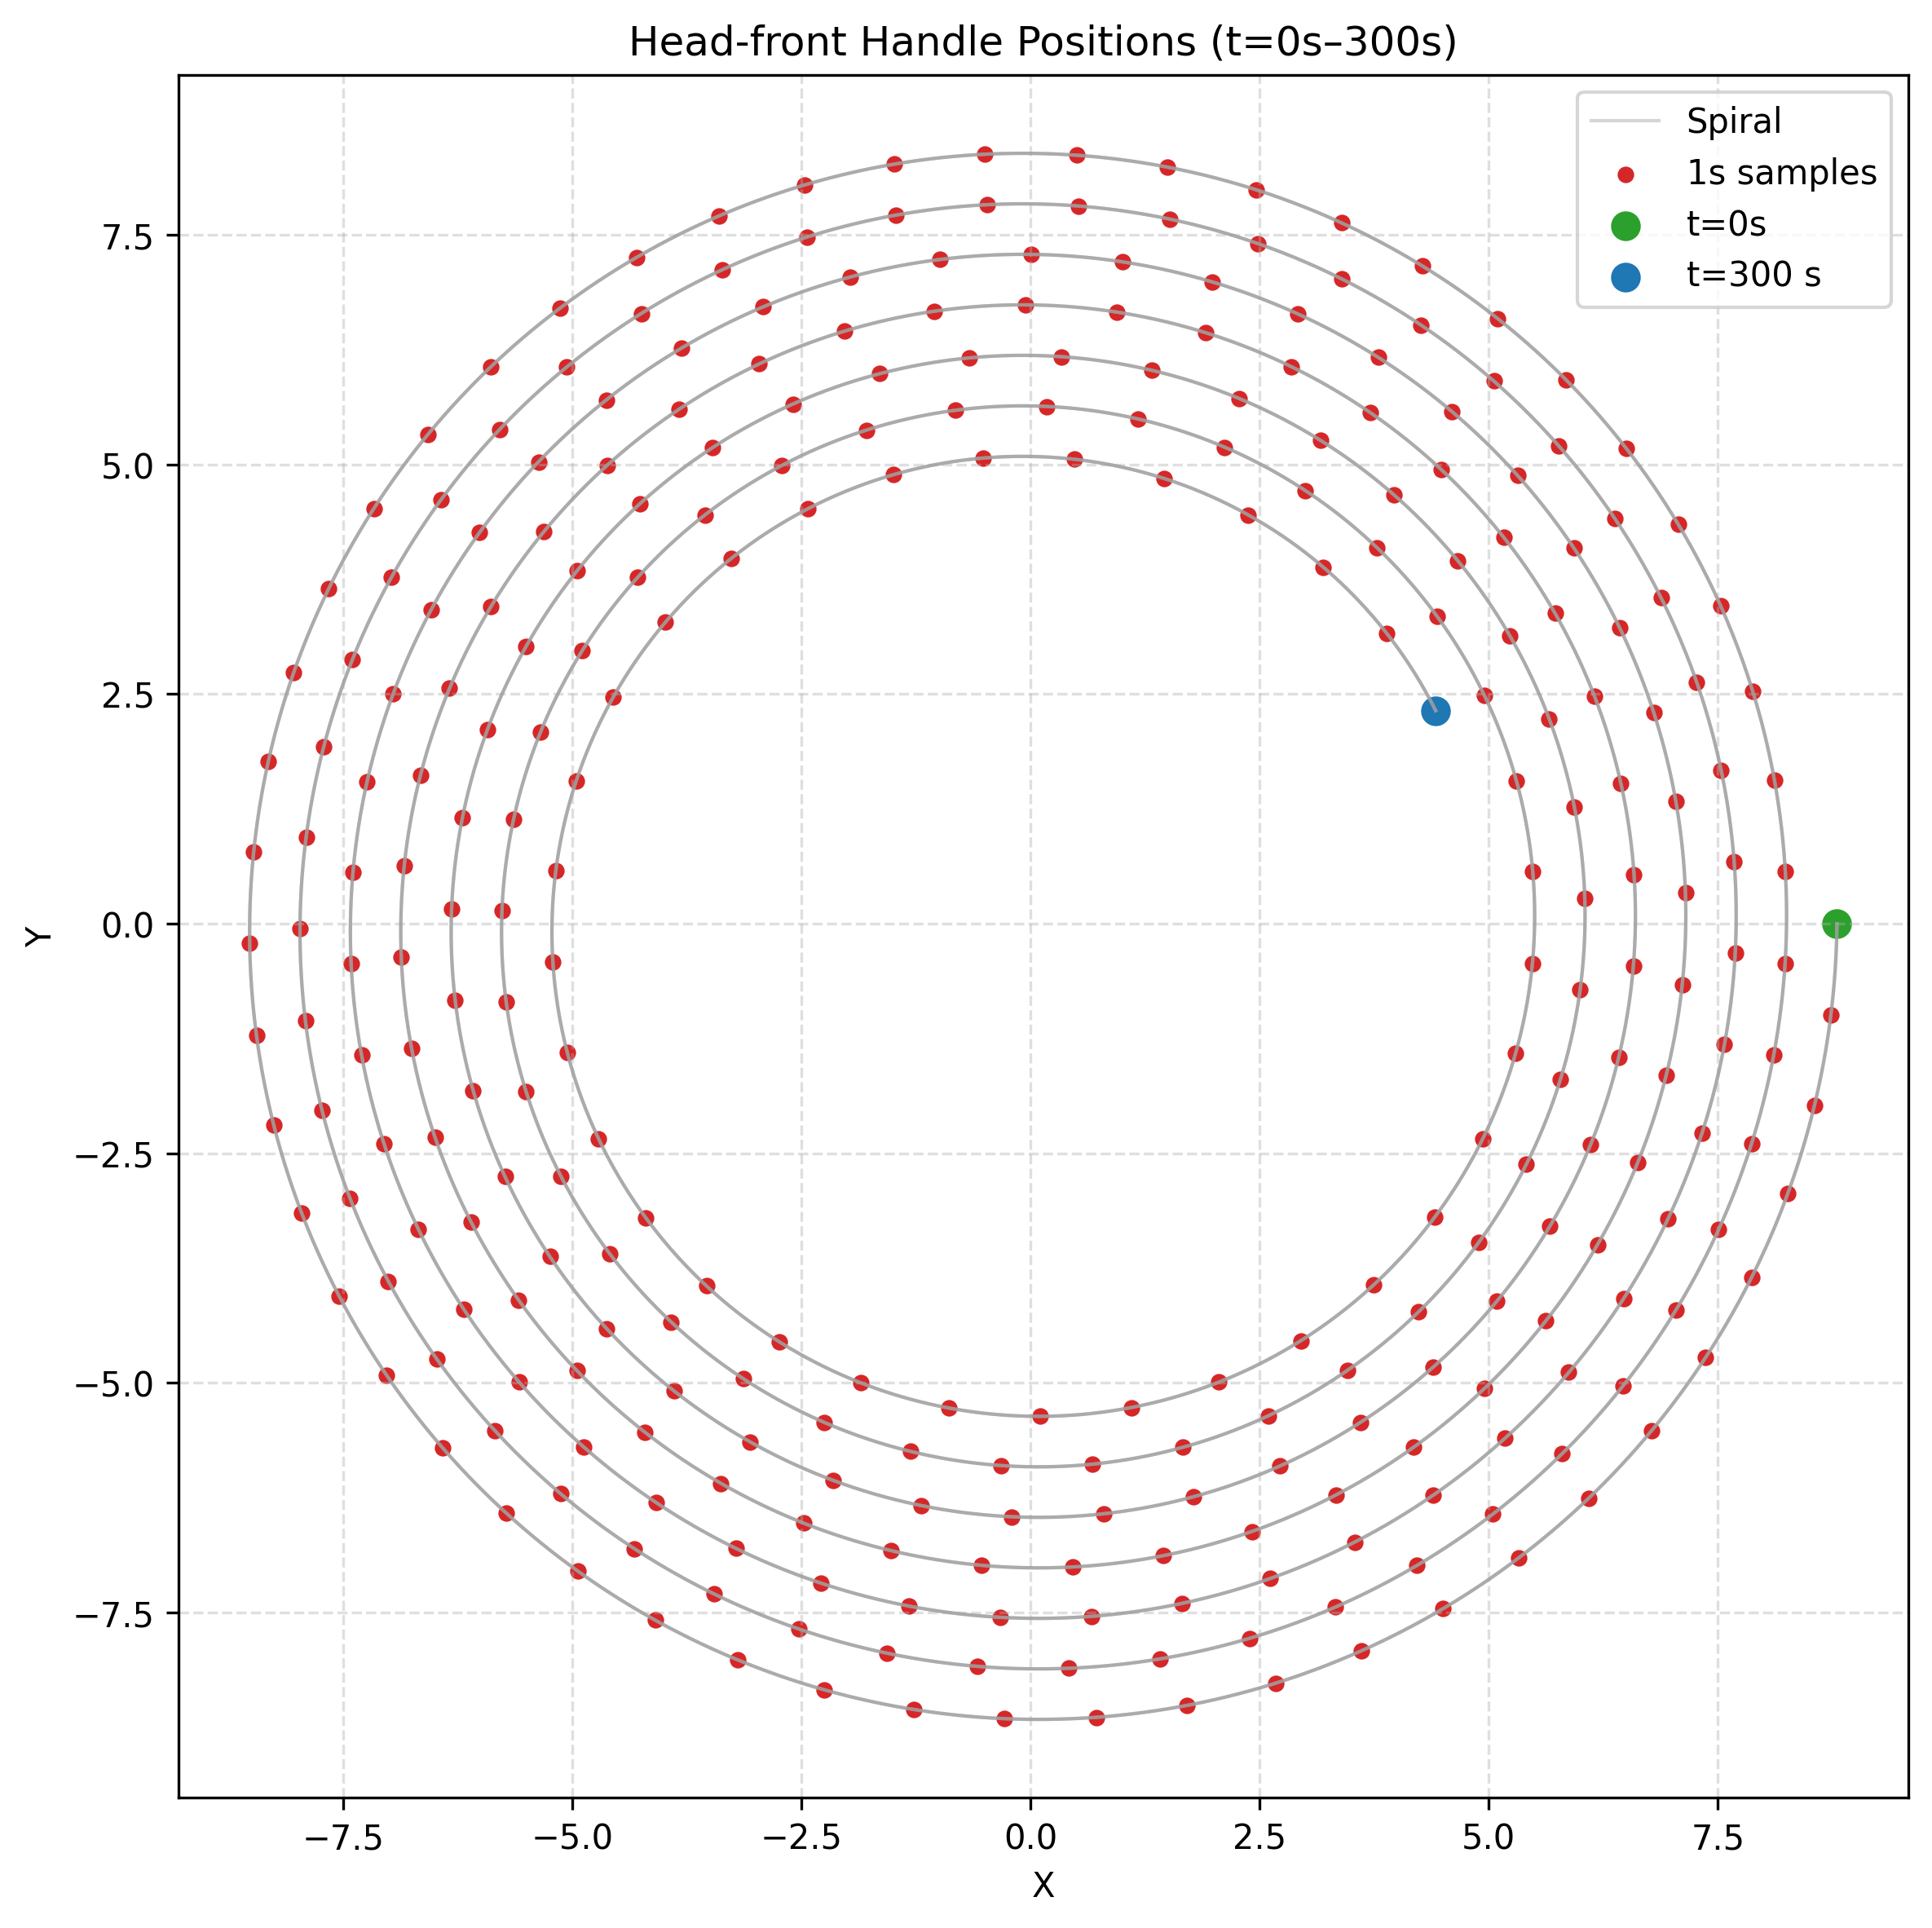
\includegraphics[width=0.70\textwidth]{图片和数据/plot3.png}
\caption{问题一龙头前把手位置散点补充图}
\label{fig:appendix_plot3}
\end{figure}

\subsection{性能优化与统一配置（project\_refactor\_improved.py）}
\paragraph{统一配置与快速根求解}
\lstinputlisting[language=Python,firstline=53,lastline=220,caption={\texttt{project\_refactor\_improved.py} 中的配置与快速根求解实现}] {project_refactor_improved.py}

\paragraph{调头路径输出图（补充）}
\begin{figure}[H]
\centering
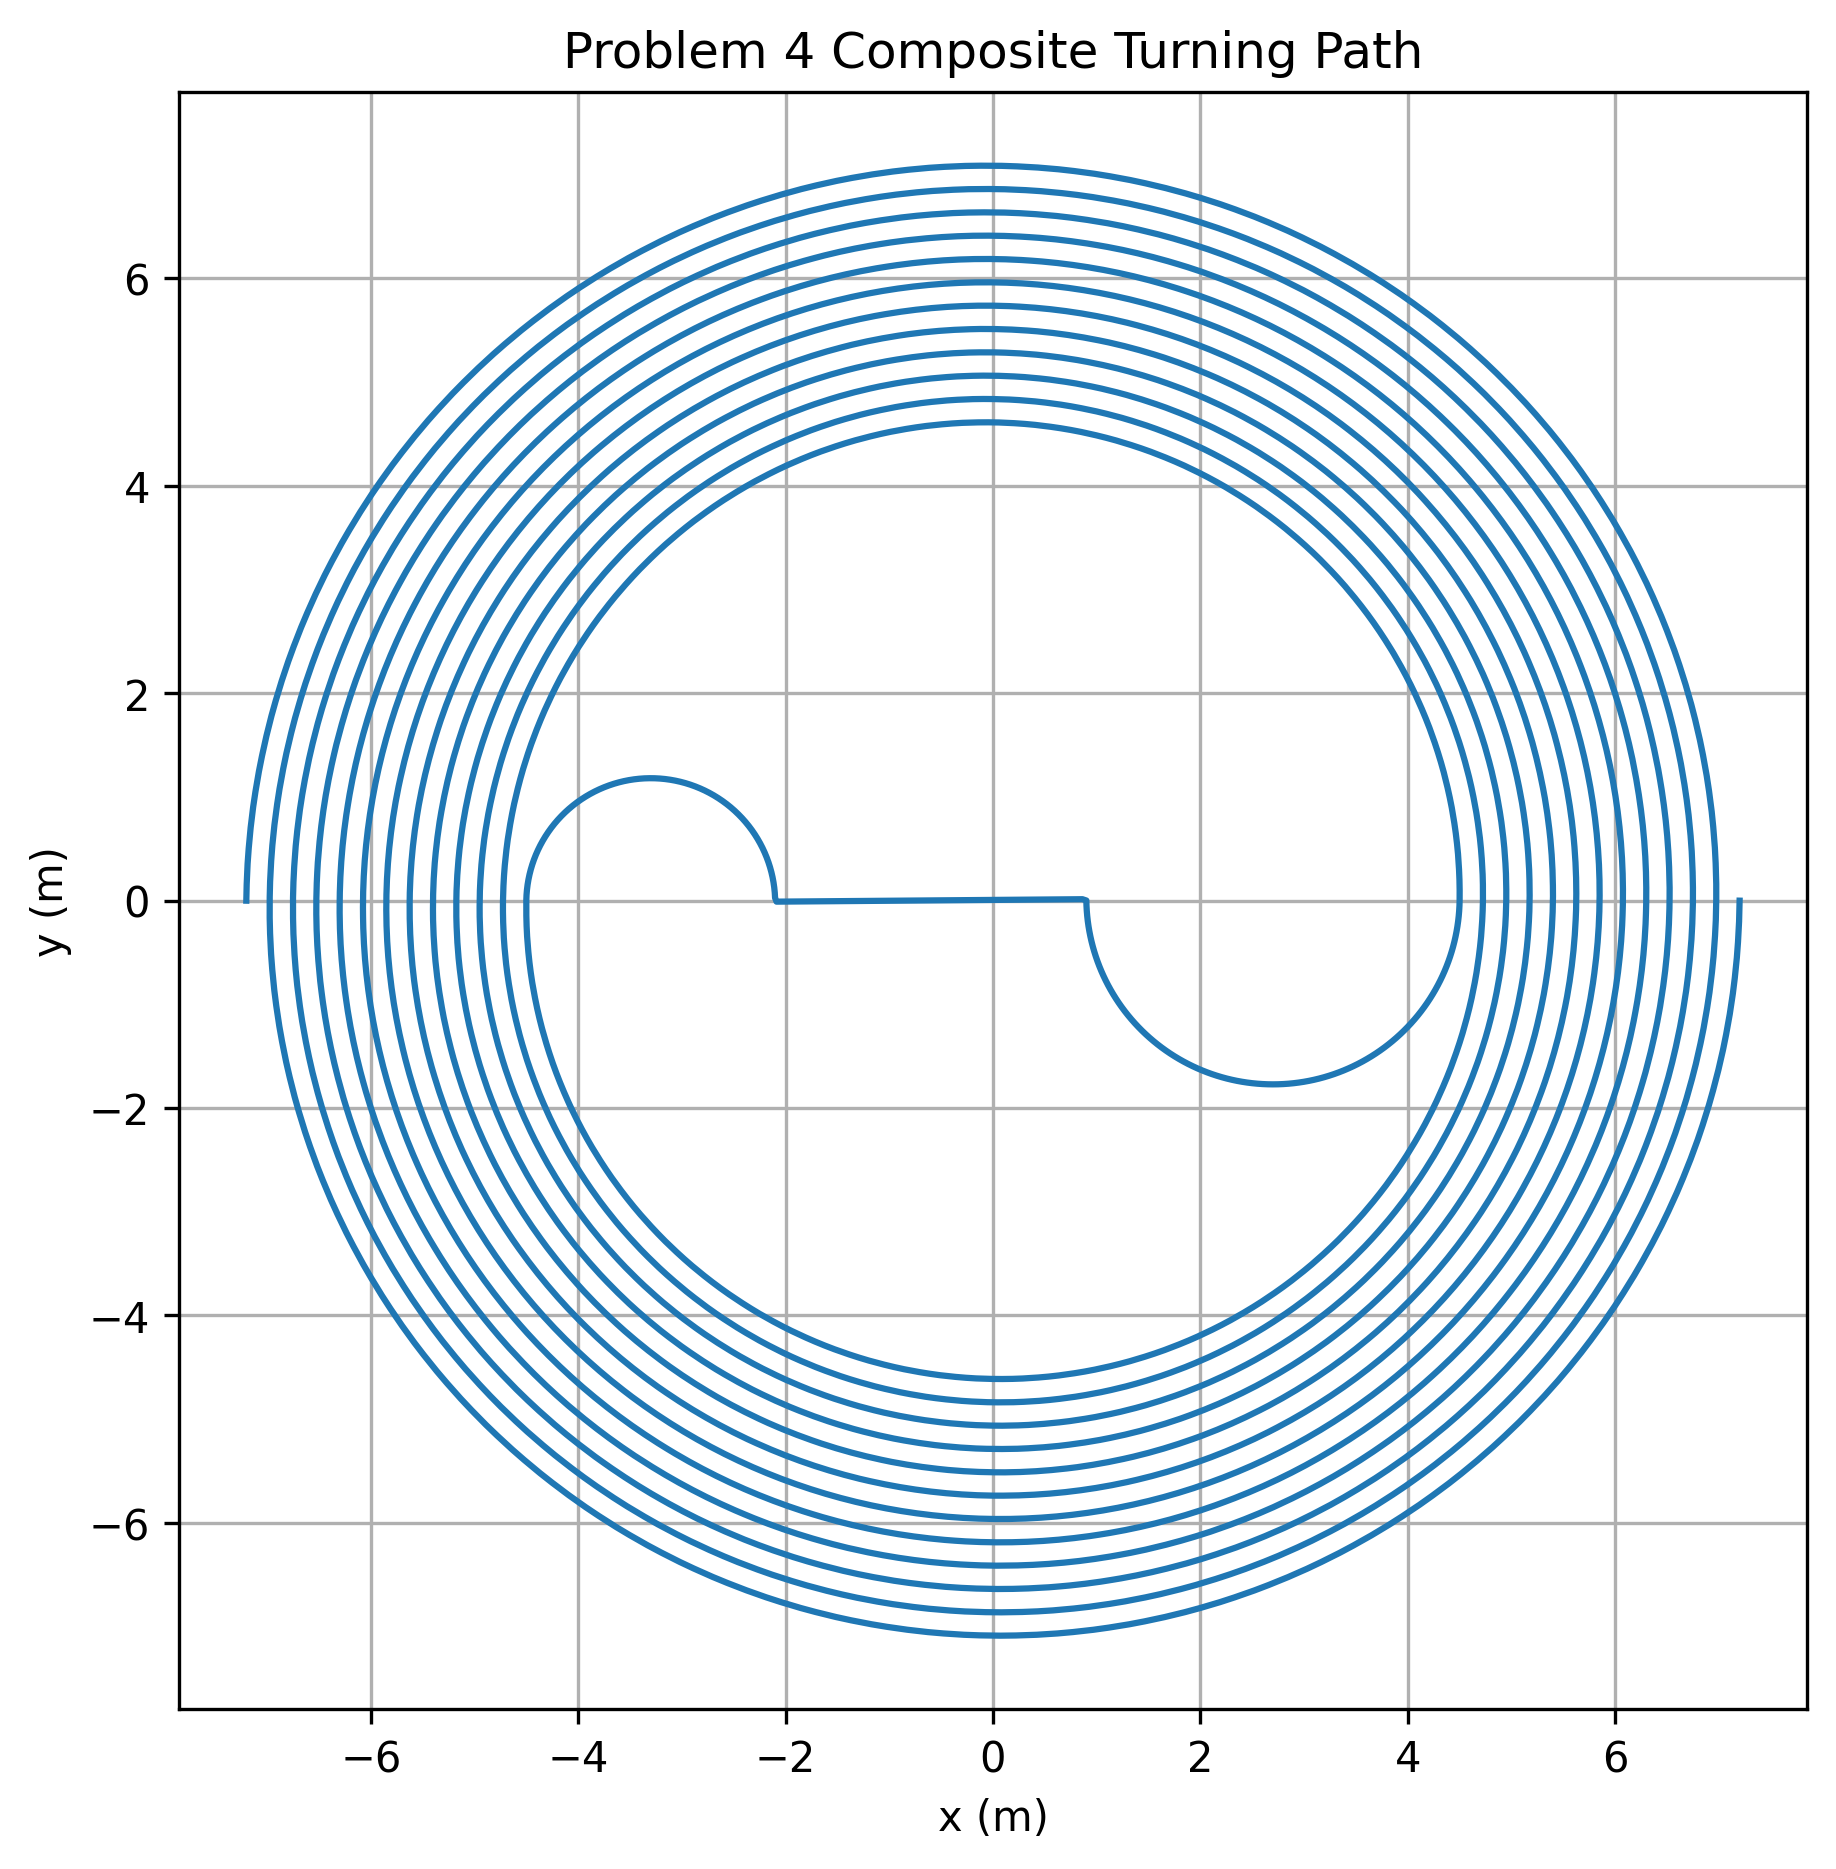
\includegraphics[width=0.75\textwidth]{图片和数据/problem4_fast_path.png}
\caption{问题四路径总览（程序原始输出图，作为补充）}
\end{figure}

\end{document}